%-------------------------------------------------------------------------------
%-------------------------------------------------------------------------------
\documentclass{brandeis-dissertation}
\usepackage{amsmath}
\usepackage{pdfpages}
\usepackage{setspace} 
\usepackage{float}
\usepackage{multicol}
\usepackage{multirow}
\usepackage{graphicx}
\graphicspath {{figures/}}
\usepackage[utf8x]{inputenc}
\usepackage{subfig}
\usepackage{indentfirst}
% package for including graphics with figure-environment
\usepackage{hyperref}
% colored borders (false) colored text (true)
\hypersetup{colorlinks=true,citecolor=blue,filecolor=black,linkcolor=blue,urlcolor=blue}
\usepackage{natbib}
%\usepackage[style=phys]{biblatex} 
%\setupttoc{toc}{numbered}
\newcommand{\Ztt}{Z\rightarrow\tau\tau}
% Add you own definitions here (file ANA-HIGG-2018-49-INT1-defs.sty).
%\usepackage{ANA-HIGG-2018-49-INT1-defs}

%-------------------------------------------------------------------------------
% Generic document information
%-------------------------------------------------------------------------------

% Title, abstract and document 
\title{\normalsize{Measurement of the vector boson fusion production Higgs boson fiducial cross-section observed in the $WW^*\rightarrow\ell\nu\ell\nu$ decay channel with the ATLAS detector}}
\author{Laura Bergsten}
\department{Department of Physics}
\advisor{Professor Gabriella Sciolla, Department of Physics, Brandeis University}
\reader{Professor Craig Blocker, Department of Physics, Brandeis University}
\reader{Dr. Alessandro Tricoli, Brookhaven National Laboratory}
%\signoff{Eric Chasalow}{Dean}
\dean{Eric Chasalow}
\graduationmonth{August}
\graduationyear{2020}
%-------------------------------------------------------------------------------
% Content
%-------------------------------------------------------------------------------
\begin{document}
%\signaturepage*
\thesisabstract{Vector boson fusion produced Higgs boson fiducial and inclusive cross-sections are measured in the $H\rightarrow WW^*\rightarrow\ell\nu\ell\nu$ decay channel using 139 fb$^{-1}$ of proton-proton collisions. Collisions from the Large Hadron Collider at $\sqrt{s}=13$ TeV are recorded by the ATLAS detector. New analysis techniques are developed to accurately estimate contamination from top decays and gluon-gluon fusion production Higgs events. An excess of vector boson fusion Higg decays are observed over Standard Model backgrounds with a significance of 6.6$\sigma$, the most conclusive observation of this Higgs production mode in the $WW^*$ channel to date. The fiducial and inclusive cross-sections are measured to be 2.78$^{+0.56}_{-0.52}$~fb and $89.2^{+18.3}_{-17.3}$~fb, respectively. No significant deviations from Standard Model predictions are observed.}
%\dedication{}
\acknowledgments{This thesis, and the entirety of my Ph.D. journey, were possible because of support and assistance from many groups and individuals, only some of which I list here. 

First, thank you to my advisor \textbf{Prof. Gabriella Sciolla}. Over the past five years, you have helped me become a better teacher, researcher, and physicist. The many hours you spent helping me practice for oral qualifiers my first year, the long walks around Brookhaven where you dispensed science and life advice, and the innumerable coffee chats at CERN, BNL, and Brandeis all pushed me to grow, learn, and finally, to finish my Ph.D.  

Thank you also to \textbf{Prof. Craig Blocker} and \textbf{Dr. Alessandro Tricoli} for serving on my thesis committee. Your comments enabled me to think more deeply about the subject matter and become a better writer. I owe additional thanks to Alessandro for leading my analysis team. Our weekly meetings encouraged me to think about problems in new ways and your guidance is evidenced throughout this thesis.  

I am grateful to the VBF $H\rightarrow WW^* \rightarrow \ell\nu\ell\nu$ differential group, whose team-wide efforts contributed to the measurements I detail here. I would especially like to thank \textbf{Dr. Gaetano Barone} and \textbf{Sagar Addepalli}; Gaetano, for teaching me how to complete a physics analysis and providing help in everything from statistics to debugging and Sagar, for taking over many of my responsibilties in the analysis and for the thoughtful questions and contributions you made in the past months. 

Next I would like to thank all my Brandeis labmates, but in particular \textbf{Prajita Bhattarai} for always saying ``yes'' to an adventure, \textbf{Dr. Hannah Herde} for her constant support and encouragement, and \textbf{Jiayi Chen} for tea breaks and friendship. 

While it only features briefly in this thesis, my time at Brookhaven National Lab was a formative experience and I appreciate the entire ITk strips community for their welcome. I want to highlight \textbf{Dr. Dave Lynn} for leading my thermomechanical stave testing efforts and \textbf{Dr. Stefania Stucci} for her mentorship at BNL.

None of this work would have been possible without the love and support of my friends and family. To my parents, \textbf{Bob and Liz,} thank you for constantly reminding me of the world beyond particle physics and cheering every accomplishment, big or small. To my grandma, \textbf{Jackie,} for instilling the importance of education in me and being my (and Nicks'!) biggest fan. To my sisters, \textbf{Lissy and Sabrina,} for understanding all of my jokes and inspiring me with all youhave each accomplished. And finally, I need to thank \textbf{Nick.} We met while I was in the midst of my first year at Brandeis and in the time that followed you took endless trips on trains, ferries, and planes to visit each new place I called home. Your confidence in me is infectious and I am at my best in your company.  I can't wait to begin the next set of adventures beside you. 
}
\thesisfront[lot,lof] %other options include onlinesubmission, copyright, nocopyright, lot, nolot, lof, nolof
\clearpage
%\begin{doublespacing}
%\cleardoubleoddpage
%\pagenumbering{roman}
%sectionnumbering{roman}
%\listoftables
%\listoffigures
%\end{doublespacing}
%\tableofcontents

%-------------------------------------------------------------------------------
%-------------------------------------------------------------------------------
%\pagenumbering{arabic}
%\sectionnumbering{arabic}
\chapter{Introduction}
\label{sec:intro}
Introduction to the thesis. Explain what u'll see.

\clearpage
%-------------------------------------------------------------------------------
%-------------------------------------------------------------------------------
%-------------------------------------------------------------------------------
\chapter{Theory}
\label{sec:theory}
\section{Standard Model}
The Standard Model (SM) is the leading theory that describes interactions between particles at a subatomic scale. I begin with a brief summary of the SM itself beginning with brief descriptions of the fundamental particles and their forces before delving into a summarized mathematical formulation. Next, I discuss the history of the SM and crucial tests of the theory up until current work at the LHC.  I will then  outline some of the recent and current physics at the Large Hadron Collider (LHC) with a focus on Higgs boson measurements. Finally, I'll introduce my thesis' main focus, differential cross-section measurements of Vector-Boson-Fusion Higgs decaying into two W-bosons.

The Standard Model is one of the most successful scientific theories to date. Its predictions encompass all of the visible universe and continue to undergo careful testing. The SM combines three forces- electromagnetic, weak, and strong - into one elegant description. I'll follow in the steps of many before me and detail the theory through first introducing particles and forces. Next I will introduce the mathematical formalisms describing particle interactions.
\subsection{Particles and forces}
 The particles we define in high energy physics are the most minute portions of matter we're able to observe. They are generally considered point-like, have no internal structure, and cannot be further split. Each particle we can define has a unique set of quantum numbers and its own anti-particle (with the same mass and spin, but opposite electrical charge and quantum numbers).

Particles can split up into distinct groups- first bosons, with integer spin, and fermions, with half-integer spin. Bosons are 'force carriers' meaning when particles interact they exchange bosons. Fermions are at the heart of all conventional matter. Fermions can be split further into two categories- leptons and quarks. Quarks have fractional integer charge and interact strongly while leptons have integer charge and interact solely through the weak or electromagnetic forces. Both quarks and leptons are made of three generations of particles, each heavier and more unstable than the next. Charts showing quark/lepton families and their key quantum numbers are shown below. Each generation of quarks and leptons contains a particle doublet. Each lepton doublet contains a charged lepton and a neutrino while each quark doublet contains one $+2/3$ charged particle and one with a $-1/3$ charge. Each lepton and quark also has an anti-particle. All conventional, stable matter is made from the first generation of quarks and leptons.

There are four gauge bosons and one scalar boson predicted through the SM. These correspond to three fundamental forces in nature (the fourth, gravity, is so small on the scale of particle interactions as to not be considered). The strongest force on the subatomic scale is the strong force- this is mediated by the gluon- and works primarly to bind quarks together to form composite particles like protons or neutrons. The electromagnetic force is about 60x weaker than the strong force and is mediated by the photon. This force accounts for all electric interactions like that between an electron an an atomic nucleus. Finally, the weak force ($10^4$ weaker than the EM) facilitates $\beta$-decay and is mediated by massive Z and W bosons. Before going into more detail on the gauge bosons and the forces they mediate, I'd be remiss not to mention the Higgs boson. The only scalar boson predicted by the SM, it is has no charge or intrinsic spin. The Higgs gives mass to all other particles through Spontaneous Symmetry Breaking, which I'll expand on in later sections.
\begin{figure}[H]
	\centering
    \includegraphics[width=0.7\textwidth] {Pictures/SMparticles.png}\hspace{1cm}
    \caption{Three generations of quarks and leptons are shown along with all SM bosons \cite{PDG}}
    \label{fig:SMparticles}
\end{figure}
Photons are massless, spin-1 particles and mediate all electromagnetic interactions. They couple directly to any particle with electric charge- so quarks, leptons, and $W$/$Z$ bosons but not neutrinos. Since the photon is massless, the electromagnetic force can operate on infinitely long scales but it's force decreases with $1/r^2.$
 
Gluons are massless particles with no charge and a spin-1. They couple to color charges, which are a property of quarks. Each quark has one of three colors (RGB) while anti-quarks have "anti" versions of these. Colors ore conserved 'charges' just like electric charge. Quarks are never found alone as they couple so strongly to one another as to be confined in groups of two or three. These groups are "color-confined" meaning the quarks contain colors which add up to a color neutral sum. For instance, a two quark meson $u\bar{u}$ may have colors R and anti-R while a three quark hadron $uud$ (proton) may have colors R, G, and B. Gluons are different from photons in that they are not neutral to the charge they couple to. Gluons have two colors (8 total combinations) and can thus couple to each other. This makes the strong force distinct from the electromagnetic and has implications for long-distance interactions.
 
$W$ and $Z$ bosons, unlike gluons and photons, are massive. However, like their other gauge boson counterparts, they have spin-1 and mediate a charge (weak). $W^{\pm}$ mediates charged-current interactions which can violate flavor conservation between quarks and/or leptons and their neutrinos. $Z^{0}$ mediates neutral-current interactions which conserve flavor. $W^{\pm}$ bosons contain electric charge so can interact through EM as well. In addition, $W$ and $Z$ bosons contain weak charge (as do all fermions) so can self-couple as well as couple with all fermions. 
 
The Higgs boson will be further motivated and described in later sections but suffice to say it's a massive spin-0 particle which couples to all particles with mass (including itself). It doesn't mediate any force but is still an integral part of the SM.  

\subsection{Gauge Invariance}
According to Noether's theorem, for every continuous transformation of a field that leaves the Lagrangian invariant, there is a conserved current. Symmetries found in physical theories lead to conservation laws (and vice-versa). The Standard Model is a gauge theory built on symmetries such that all interactions between particles result from requiring the theory to be invariant under local gauge transformations. Each part of the Standard Model- from quantum electrodynamics (QED) to quantum chromodynamics (QCD) - is a gauge theory on its own, which simply means they have gauge invariance symmetries. In this section I'll step through the basic mathematic formalism for QED, QCD, and the combined electro-weak theory to illustrate the physical ramifications of gauge invariance and set the stage for the Higgs mechanism. The following sections are written with guidance from text \cite{HalzenMartin}. 

\subsubsection{Quantum Electrodynamics}
Quantum electrodynamics (QED) is the first, and simplest, physical gauge theory, describing how light and matter interact even under relativistic conditions. The theory produces extremely good agreement with experiment due to the success of perturbative solutions and entire textbooks are dedicated to its motivation and calculated predictions. Here I will generate the full QED Lagrangian by imposing local gauge invariance on the Lagrangian of a free fermion. 

First, the Dirac Lagrangian describes a free fermion of mass \textit{m}
\begin{equation}
\mathcal{L} = i \psi \gamma^\mu \partial_ \mu \psi - m\bar{\psi}\psi,
\end{equation}
where $\psi$ is a Dirac spinor and $\gamma^\mu$ represent the Dirac matrices. To demonstrate local gauge invariance we need to transform
\begin{equation}
\psi(x) \rightarrow e^{i\alpha(x)}\psi(x) 
\end{equation}
where $\alpha(x)$ depends on space and time arbitrarily. Directly substituting this into our Lagrangian shows that $\mathcal{L}$ is not invariant, and the $\partial_\mu$ term breaks this
\begin{equation}
\partial_\mu \psi \rightarrow e^{i\alpha(x)}\partial_\mu\psi + ie^{i\alpha(x)}\partial_\mu \alpha
\end{equation}
In order to mandate the theory is invariant we need to change this term to the "covariant derivative" $D_\mu$ which transforms 
\begin{equation}
D_\mu\psi \rightarrow e^{i\alpha(x)}D_\mu\psi . 
\end{equation}	 
In order to transform as such the "covariant derviative" has to contain a vector field $A_\mu$ and this field must transform so as to cancel with the unwanted part of the transformed $D_\mu$. 
\begin{equation}
D_\mu \equiv \partial_\mu - ieA_\mu
\end{equation}
where 
\begin{equation}
A_\mu \rightarrow A_\mu + \frac{1}{e}\partial_\mu \alpha
\end{equation}
Now the original Dirac equation is replaced with the following:
\begin{equation}
\mathcal{L} = \bar{\psi}(i\gamma^\mu\partial_\mu-m)\psi + e\bar{\psi}\gamma^\mu\psi A_\mu.
\end{equation}
By requiring local gauge invariance we've introduced a gauge field $A_\mu$ which couples to the Dirac particle just as the photon. In fact, if we take this as the photon gauge field and so add a kinetic energy term (which is also local gauge invariant!) we find the Lagrangian of QED. 
\begin{equation}
\mathcal{L} = \bar{\psi}(i\gamma^\mu\partial_\mu-m)\psi + e\bar{\psi}\gamma^\mu\psi A_\mu -\frac{1}{4} F_{\mu\nu}F^{\mu\nu}
\end{equation}
One can also see that adding a mass term to the Lagrangian for the new field ($\frac{1}{2}m^2A_\mu A^\mu$) would break gauge invariance, indicating the photon must be massless. From the free fermion Lagrangian, imposing local gauge invariance leads to the full interacting field theory of QED. This isn't a curiosity but an essential component of the theory, and the use of local gauge symmetry in deriving particle interactions doesn't end here.
\subsubsection{Quantum chromodynamics}
Quantum chromodynamics differs from QED in a few crucial ways. First, since quark color fields exist the QED $U$(1) gauge group is replaced with $SU$(3) and the free Lagrangian contains indices $j$ to denote the three color fields. 
\begin{equation}
\mathcal{L} = \bar{q}_j(i\gamma^\mu\partial_\mu - m)q_j.
\end{equation}
QCD also carries three quark flavors, which will be ignored here for simplicity. The QCD group is also non-Abelian since not all generators of the group commute with each other. These generators will be defined as $T_a$ where $=1,...,8$ and are linearly independent traceless $3\times3$ matrices (the Gell-Mann matrices $\lambda_a$ are conventional). The local color phase transformation required is thus 
\begin{equation}
q(x) \rightarrow e^{i\alpha_a(x)T_a}q(x)
\end{equation}
We can consider an infinitesimal phase transformation as 
\begin{equation}
q(x) \rightarrow [1+i\alpha_a(x)T_a]q(x), \\
\partial_uq \rightarrow (1+i\alpha_aT_a)\partial_\mu q + i T_a q \partial_\mu \alpha_a.
\end{equation}
Just as in the QED example, the last line breaks the invariance of $\mathcal{L}$ and we can proceed very similarly to the QED case by introducing a new gauge field (or in this case eight) called $G_\mu^a$ which transform 
\begin{equation}
G_\mu^a \rightarrow G_\mu^a - \frac{1}{g}\partial_\mu\alpha_a - f_{abc}\alpha_b G_\mu^c
\end{equation}
The last term added here is to cope with the non-Abelian nature of QCD (that not all the generators $T_a$ commute with each other). Just as in QED this invariance forms a covariant derviative 
\begin{equation}
D_\mu = \partial_mu + i g T_aG_\mu^a
\end{equation}
Replacing the derivative into our Lagrangian and adding a gauge invariant energy term for each of the $G_mu^a$ fields ($\frac{1}{4}G_{\mu\nu}^aG_{\mu\nu}^a$) yields the final gauge invariant QCD Lagrangian
\begin{equation}
\mathcal{L} = \bar{q}(i\gamma^\mu\partial_\mu - m)q - g(\bar{q}\gamma^\mu T_aq)G_\mu^a-\frac{1}{4}G_{\mu\nu}^aG_{\mu\nu}^a.
\end{equation}
Just as in the QED case, imposing local color phase invariance produced a new interacting field (or rather, eight) with a coupling specified as $g$. These are the gluon fields and just like photons, local gauge invariance requires them to be massless. Unlike the QED case, this Lagrangian's new kinetic term includes self-interaction between the gauge bosons - another key feature of QCD that is mandated by local color phase invariance. Gluons themselves must carry color charge and so self-couple - the structure of these self coupling terms and their single coupling strength $g$ are uniqely determined by gauge invariance. 
\subsubsection{Electro-weak unification?}

\subsubsection{Spontaneous Symmetry Breaking}
Unlike QED and QCD, the weak force is mediated by massive gauge bosons. Because of this, we can't apply the same gauge invariance prescription that we did in the last sections. If a mass term is added to the Lagrangian we break the gauge invariance we aimed to find. If we instead ignore the gauge invariance and add a mass term to the Lagrangian, all predictive power of the theory is lost due to unrenormalizable divergences. With "spontaneous symmetry breaking" we can gain massive gauge bosons while maintaining the integrity of the theory. In this section I first describe the "spontaneous symmetry breaking" mechanism is terms of an Abelian theory composed of complex scalar fields to illustrate the overall strategy. This mechanism is then applied to the non-Abelian electroweak theory to gain massive weak gauge bosons $W^{+/-}$ and $Z$, with the Higgs field appearing as a 'spontaneous' result.

The Lagrangian for a $U$(1) gauge symmetry 
\begin{equation}
\phi \rightarrow e^{i\alpha(x)}\phi
\end{equation}
As in the QED case, we introduce a gauge field $A_\mu$ and covariant derivative $D_\mu = \partial_\mu - ieA_\mu$ to obtain the gauge invariant Lagrangian
\begin{equation}
\mathcal{L} = (\partial^\mu+ieA^\mu)\phi^*(\partial_mu-ieA_\mu)\phi-\mu^2\phi^*\phi-\lambda(\phi^*\phi)^2-\frac{1}{4}F_{\mu\nu}F^{\mu\nu}.
\end{equation}
In this example if $\mu^2>0$ we gain back the QED Lagrangian for a charged scalar particle of mass $\mu$ - with an additional self-interaction term. However, if we take $\mu^2<0$ the potential $V(\phi^*\phi)=\mu^2\phi^*\phi-\lambda(\phi^*\phi)^2$ now has a non-zero vacuum expectation value (v.e.v.) and there's a set of equivalent minima shown in Figure \ref{fig:HiggsPotential}. Choosing one of these minima spontaneously breaks the potential's rotational symmetry. Next, we can perturbatively expand the field about a minima through
\begin{figure}[H]
    \centering
    \includegraphics[width=0.5\textwidth] {Pictures/HiggsPotential.png}\hspace{1cm}
    \caption{Higgs potential when $\mu^2<0$, choosing a minima spontaneously breaks the $U$(1) rotational symmetry \cite{HiggsPotential}}.
    \label{fig:HiggsPotential}
\end{figure}

\begin{equation}
\phi(x) =\sqrt{\frac{1}{2}[\nu+\eta(x)+i\xi(x)]}
\end{equation}
Substituting this perturbation gives the new Lagrangian
\begin{equation}
\mathcal{L}'=\frac{1}{2}(\partial_\mu\xi)^2+\frac{1}{2}(\partial_\mu\eta)^2-\nu^2\lambda\eta^2+\frac{1}{2}e^2\nu^A_\mu A^\mu-e\nu A_\mu \partial^\mu\xi-\frac{1}{4}F_{mu\nu}F^{\mu\nu} + \textnormal{interaction terms}.
\end{equation}
Three particles seem to emerge here: massless Goldstone boson $\xi$, massive vector $A_\mu$ with $m_A=e\nu$ and a massive scalar $\eta$ with $m_\eta=sqrt{2\lambda\nu^2}$. However, the number of particles does not correspond to the polarization degrees of freedom expected, a longitudonal polarization was added, creating an unphysical field. To eliminate the unphysical field we can substitute new set of fields 
\begin{equation}
\phi \rightarrow \sqrt{\frac{1}{2}(\nu+h(x))e^{i\theta(x)/\nu}}
\end{equation}
and 
\begin{equation}
A_\mu \rightarrow A_\mu + \frac{1}{e\nu} \partial_\mu\theta.
\end{equation}
Introducing these substitutions, the Goldstone boson field disappears
\begin{equation}
\mathcal{L} = \frac{1}{2}(\partial_\mu h)^2 -\lambda\nu^2h^2+\frac{1}{2}e^2\nu^2A_\mu^2-\lambda\nu h^3-\frac{1}{4}\lambda h^4+\frac{1}{2}e^2A_\mu^2h^2+\nu e^2A_\mu^2h-\frac{1}{4}F_{\mu\nu}F^{\mu\nu}
\end{equation}
Here the degrees of freedom before our substitutions remains the same and a massive boson $A_\mu$ is preserved along with a massive scalar $h$. The "Higgs mechanism" applied to a scalar field succeeded in creating a massive boson and determined the existence of a Higgs boson. One can apply the same mechanism to the more complicated $SU$(2) gauge symmetry of electroweak interactions to determine the mass of the $W$ and $Z$ bosons and predict the existence of the Standard Model Higgs boson. 


\section{Brief history of SM tests}

\section{LHC Physics/Phenomenology}

\section{Measurement motivation}


\clearpage
%-------------------------------------------------------------------------------
%-------------------------------------------------------------------------------
%-------------------------------------------------------------------------------
\chapter{The LHC and the ATLAS detector}
\label{sec:LHCandATLAS}
 
The Large Hadron Collider (LHC) is a proton-proton storage ring operating at CERN and for its 9 years of operation, it has been the world's highest energy particle collider. 
%The LHC first began operation in 2008 but following a magnetic quench incident it had to be repaired and adjusted. The first data-taking commenced in 2009 \cite{Rossi_2010}. 
During LHC operation thus far, protons have collided with increased center-of-mass approaching the design energy of 14 TeV. Instaneous luminosity has also successively increased, surpassing design instaneous luminosity of $1\times10^{34}$cm$^{-2}$s$^{-1}$ in 2018 to reach $2\times10^{34}$cm$^{-2}$s$^{-1}$\cite{CERNnews1}. The overall data recorded in the ATLAS detector totals more than $10^{16}$ collisions. Operation of the LHC has led to the discovery of the Higgs boson and some of the most precise measurements of its properties including the coupling of the Higgs boson to bottom quarks \cite{Aaboud_2018_0}, $W$ and $Z$ bosons \cite{Aaboud_2019}, \cite{Aaboud_2018}, photons\cite{Aaboud_2018_2} and tau leptons \cite{Aaboud_2019_2}. The LHC has also facilitated searches for new physics over a wide parameter space, setting confidence level exclusion limits on masses of supersymmetric particles like squarks, gluinos and neutralinos \cite{ATLAS-CONF-2019-040}. 

The LHC can run continuosly for a few years before detector components need to be repaired and replaced. The schedule of data-taking consists of long periods of data accumulation (Run 1 from 2015-1016, and Run 2 from 2017-2018) paired with long shutdown periods. The LHC is set to begin Run 3, in which design center-of-mass energy should be reached, in 2021. Following Run 3 detector upgrades will be installed during a long shutdown. Then the High-Luminosity LHC (HL-LHC) will begin colliding protons with unprecedented ($10\times$) luminosity in 2027 \cite{CERNnews2}. The HL-LHC and its goals will be explained further later in this chapter. Suffice to say LHC-physics is progressing quickly and promises exciting developments in the near future. 

In a brief explanation of the LHC operation, one could begin with the small volume of $\approx 10^{11}$ protons that are accelerated per bunch. Linac-2 is the primary accelerator for CERN colliders and has been since the early 1990s \cite{LHCInjector}. This injects protons at 50 MeV into the Proton Synchrotron Booster (PSB) where they are further accelerated to 1.4 GeV. In the the Proton Synchrotron (PS), the protons are separated into bunches with a spacing of 25 ns and are futher accelerated to 25 GeV before being extracted to the Super Proton Synchrotron (SPS), where they reach 450 GeV. Finally the bunches of protons enters the LHC, where they are accelerated to their final energy of 6.5 TeV. Linac 2, PSB, PS, and SPS were all operational accelerators before the LHC era though each had to be majorly upgraded to handle the energy and beam intensity required for LHC collisions \cite{LHCInjector}. 

The LHC layout mimics that of the Large Electron Positron collider (LEP) that was housed in the same tunnels. Figure \ref{fig:LHClayout} shows the positioning of each experiment at the LHC as well as injection systems and other features. Once proton bunches enter the LHC in two opposing beams, they are accelerated with radio frequency (RF) systems. Located at Point 4 in the LHC schematic, the system consists of 16 RF cavities operating at twice the frequency of the SPS injector. RF cavities are metallic chambers containing oscillating electromagnetic fields; in the LHC this oscillation frequency is 400 Mz. The tuning of this frequency ensures that protons of the ideal energy are not accelerated further and simply maintain their momentum while particles arriving in an RF cavity slightly before or after will be decelerated or accelerated toward the ideal proton energy. This acceleration process can also be used to split beams of protons into discrete bunches, and this is first done with RF cavities in the PS. After proton bunches have circled the LHC approximately 1 million times (15 minutes), peak energy is reached and collisions can commence \cite{radiofrequency}.

\begin{figure}[!h]
        \centering
    \includegraphics[width=.6\textwidth]{Pictures/LHClayout.PNG}
    \caption{LHC layout \cite{LHCref}}
    \label{fig:LHClayout}
\end{figure}

Superconducting magnets in the LHC main dipoles create a magnetic field of $\approx 8$ T to bend the proton beams into the circlular path of the collider. Figure \ref{fig:dipolemagnet} shows the flux in a dipole cross-section. The opposing direction beamlines are shown centered and the flux is shown to be high (and directionally opposed) in the center of each beam. To maintain these fields, the magnets operate at below 1.9K. Pressurized superfluid helium chosen for its low visosity and high specific heat cools the dipole magnets. Once the two LHC rings are filled from the SPS the center-of-mass energy of the beams increases until it reaches peak energy after about 28 minutes. Finally, proton bunches separated by 25ns collide simultaneously in each detector.  

\begin{figure}[!h]
        \centering
    \includegraphics[width=.6\textwidth]{Pictures/dipolemagnet.jpg}
    \caption{ Flux within an LHC dipole cross-section \cite{LHCref}}
    \label{fig:dipolemagnet}
\end{figure}

\section{ATLAS, A Toroidal LHC ApparatuS}
\hspace{20pt} The LHC creates proton-proton collisions at the rate and energy necessary for pushing the boundaries of particle physics, but identifying and reconstructing the tracks of such energetic particles is no mean feat. A Toroidal LHC ApparatuS (ATLAS) and the Compact Muon Solenoid (CMS) are multi-purpose detectors built to search for a wide range of particle interactions and the measurement of their properties. Both experiments measured a particle consistent with the Higgs boson in 2012 and their agreement was a key verification of the discovery. The following sections describe each major component of the ATLAS detector so to highlight their role in the measurement of Higgs$\rightarrow WW \rightarrow \ell\nu\ell\nu$. 

ATLAS utilizes a coordinate system with its origin at the center of the detector (the ``interaction point") and has a z-axis along the beam pipe. The x-axis points from the interaction point to the center of the LHC ring, and the y-axis points upward. The experiment uses cylindrical coordinates $(r, \phi)$ where $\phi$ is the azimuthal angle around the beam pipe. The pseudorapidity and the transverse momentum are defined in terms of the polar angle $\theta$ as $\eta = -\ln( \tan(\theta/2))$ and $p_T = p\sin\theta$. 
\begin{figure}[!h]
	\centering     \includegraphics[width=.7\textwidth]{Pictures/ATLASdetector.PNG}
    \caption{Computer-simulated ATLAS detector schematic \cite{detector}}
\end{figure}

The Inner Detector (ID) detects charged particles with $|\eta| < 2.5$ operating in a 2 T solenoidal field. It consists of $3$ layers of pixel sensors, $4$ layers of silicon strips, and $72$ straw layers of transition radiation tracker modules. The ID describes particles closest to the interaction point and locates track parameters with great resolution due to its high granularity \cite{detector}. 

The ATLAS detector contains 3 superconducting magnet systems- the central solenoid, barrel toroid, and 2 end-cap toriods. The central solenoid provides a magnetic field for the inner detector while the toroids create a strong magnetic field for for the muon detector. These magnets were built to create the largest possible uniform magnetic field to maximize the momentum resolution on particle tracks. They also need to use as little material as possible so as to not unduly influence particles in the detector. The toroids in the barrel and endcap each have 8 coils and create a 4 T magnetic field while the central solenoid creates a 2 T magnetic field in the inner detector. Combined the magnet systems contain $>$100 km of superconducting wire which are cooled to working temperatures below 5K \cite{detector}. 

The Muon Spectrometer precision chambers provide muon momentum measurements at a high resolution over a wide range of $p_T$. The MS consists of $3$ layers of Monitored Drift Tube chambers covering $|\eta| < 2.7$ and an inner layer of Cathode Strip Chambers with $|\eta| > 2.0$. In addition, it includes trigger chambers that contain $3$ layers of Resistive Plate Chambers ($|\eta| < 1.05$) and $3$ layers of Thin Gap Chambers ($1.05 < |\eta| < 2.4$). As the outermost subdetector, the MS provides precise muon momentum measurements along the muon trajectory and the muon chambers are located with a precision of under $60$ $\mu m$. The MS also contains a system of three superconducting toroidal magnets each with eight coils providing a magnetic field with a bending integral of up to $6$ Tm \cite{detector}. 

Calorimeters provide detailed information about the energy deposited as particles pass through. Electromagnetic calorimeters detect and halt the motion of electrons and photons while the hadronic calorimeter does the same for hadrons. Muons and neutrinos are able to pass through the calorimeters to the MS. The electromagnetic and hadronic calorimeters, made of liquid Argon and scintillating tiles respectively, are able to pass information from the location of energy deposits to the various idenfication and reconstruction algorithms \cite{detector}. 

\section{The High-Luminosity LHC and Inner Tracker (ITk)}
The LHC succeeded in its paramount goal of discovering the Higgs boson in 2012. Its continuous operation at higher energy and luminosity has led to more rigorous measurements of Higgs boson properties as well as searches for new physics beyond the Standard Model. While more data collection is planned in Run-3 starting in 2021, new colliders and detectors take decades to design, develop and build, so the plans for upgrading the current detectors are well underway. The High Luminosity LHC will operate at 14 TeV starting in 2027. The HL-LHC will begin with $5-7\times$ the luminosity of the LHC and peak at the design instaneous luminosity of $10\times$ the LHC, or $12.6\times10^{-34}$cm$^{-2}$s$^{-1}$. This huge increase in number of collisions requires substantial upgrades to the LHC including new 11-12 T superconducting magnet systems, compact superconducting cavities for beam rotation and phase control, and new technology beam collimation \cite{HLLHCYellow}. 

Just as the LHC had to be re-designed, so too do all the experiments to be able to handle the much higher luminosity. The detectors must be built to withstand more radiation, as the increased collision rate also means a high radiation rate, especially closest to the beamline. They also have to provide greater granularity to be able to reconstruct tracks with good enough resolution that individual tracks can be discriminated. Finally, they have to faster to be able to deal with increased pile-up. Pile-up is caused by high numbers of collisions occuring at each bunch crossing. When there is a large amount of pile-up it becomes difficult to trace which particle tracks come from the same interaction point. Finally, the increased data in and of itself creates a complex problem for the detectors to solve. The trigger system must quickly select and store the events that may hold interesting information. 

Detectors for high energy colliders are not built often - expensive and time-consuming to design and test, they are made to last at least a decade. I was lucky to have the opportunity to work on ATLAS detector research and development during the 1.5 years I worked at Brookhaven National Laboratory during my Ph.D. Though my thesis is not directly related to this work, it was formative and extremely interesting, so I touch on this in the next section. Because I worked on the new ATLAS Inner Detector for the HL-LHC (termed Inner Tracker or ITk) I will discuss solely this sub-detector and the particular role I played in its assembly.

\subsection{Inner Tracker (ITk)}
The Inner Tracker is planned to be an all-silicon detector that will completely replace the current Inner Detector.  While the current ID has been extremely successful during Runs 1 and 2 (and will certainly continue to be in Run 3), it does not have the capacity to withstand the radiation and pile-up conditions of the HL-LHC. The ITk is designed to operate for 10 years under an instantaneous luminosity of 7.5$\times10^{-34}$cm$^{-2}$s$^{-1}$ with 25 ns between bunch crossing. This will result in 1,000 fb$^{-1}$ and average pile-up up to $<\mu>=200$ \cite{ITktech}. The current solenoid magnet will remain in the detector with a 2 T magnetic field. The ITk will consist of an innermost section with silicon pixels and an outermost section of silicon strips. The pixel detector will contain four barrel layers and six forward region disks, while the strip detector will contain five barrel layers and seven disks. The rapidity range matches the coverage of the Muon Spectrometer with $|\eta|<2.7$. This layout is shown in \ref{fig:ITklayout}. 
\begin{figure}[!h]
        \centering
    \includegraphics[width=.6\textwidth]{Pictures/ITklayout.png}
    \caption{ ITK layout as defined in ITk Technical Design Report \cite{ITktech}}
    \label{fig:ITklayout}
\end{figure}

\subsubsection{Building ITk Strip barrel staves}
At Brookhaven National Laboratory, I made key contributions to the ITk Strip barrel stave assembly effort. The goal of stave assembly is to glue silicon modules to carbon fiber stave cores within a 25 $\mu$m tolerance. Brookhaven is responsible for assembly of 200 ITk staves and their accurate assembly is necessary for the ITk to reduce uncertainty on track positions as well as to ensure a symmetric detector. I was tasked with co-creating a stave assembly software system through LABView to automatically calibrate required module positions, apply a layer of adhesive gel, and guide a user in accurately placing a module into its specified location. This project was highly collaborative and evolved further after I left the laboratory, but the overall process remains unchanged.

The basic design of the Inner Tracker for both barrel and endcap components is the same - a carbon fiber core (containing titanium cooling pipes) is covered on each side with co-cured kapton service tapes. The carbon fiber core is designed to reduce material inside the detector and the similar design in the barrel and endcap adds to simplicity. Silicon modules are glued to stave cores. Similar silicon strip detectors have been used previously in both ATLAS and CMS, but have never covered so much fiducial area. The modules consist of one silicon sensor and one or two low-mass PCB's (hybrid) which host ASICs. Module design has optimized producibility and low cost while maintaining readout goals. Overall module design is the same in barrel and endcap regions, while strip lengths and geometries vary. Components of a short-strip barrel module are shown in \ref{fig:module}.
\begin{figure}[!h]
        \centering
    \includegraphics[width=.4\textwidth]{Pictures/ITkmodule.png}
    \caption{Short-strip barrel module components \cite{ITktech}}
    \label{fig:module}
\end{figure}
 
Each barrel stave core needs to be ``loaded" with 14 modules, as shown in the assembled electrical prototype in \ref{fig:stave}. 

\begin{figure}[!h]
        \centering
    \includegraphics[width=.8\textwidth]{Pictures/electricalstave.png}
    \caption{Electrical stave prototype at Brookhaven National Laboratory (G. van Nieuwenhuizen)}
    \label{fig:stave}
\end{figure}

Brookhaven National Laboratory is one of two sites responsible for assembling barrel staves. Assembly procedures have been tested with the production of numerous prototypes including a thermomechanical double-sided stave and a fully operational electrical stave. The thermomechanical prototype was later used for various thermal tests, including IR imaging. The electrical stave was used for testing the full electrical read-out. Stave assembly is composed of three main parts: system calibration, module placement, and survey of results. 

Staves at BNL are assembled on a granite table housing an Aerotech XYZ Stage accurate to the micron level. The stage is equiped with a 10-megapixel camera that gives real-time feedback to a nearby computer and a glue dispenser. The stave assembly software system is implemented by a user who interacts with a LabView GUI and monitors progress. The stave is fixed to optical rails drilled into the granite table. In order to accurately place modules in their correct positions a series of calibrations need to be completed including camera calibrations to test the optimal working point, focus, and pixel-to-micron conversion. Next, the position of the stave with relation to the XYZ stage needs to be calibrated. Tranforming coordinates of the XYZ stage to that of the stave requires locating a fixed point on the stave core as well as the angle of the stave relative to the XYZ stage. Pattern matching algorithms find the exact locations of particular features on the stave core and allow calculation of required positions for all modules based on specifications. Once specified, module positions are calculated, calibrations are completed and it is time to apply glue and afix modules. 

Next, an epoxy (SE4445) is loaded into the glue dispenser on the XYZ-stage which is connected to a vaccuum controlled by the LABView software system. The epoxy is automatically dispensed in lines to cover $\approx$ 60\% of area under the module. Then the module is lifted with a custom-made ``pick-up" tool which uses vacuum applied to module corners to hold the module in place and move it to the needed position along the optical rails. Using real-time feedback from the software system and its pattern matching algorithm, the user is directed on how to finetune module position using knobs on the ``pick-up" tool. Markings etched in the silicon sensor at each corner are used to position the module accurately. The output of the module alignment GUI is shown in \ref{fig:modulealignment}. When the module is within specifications it is lowered into position above the epoxy and held in place for 24 hours until the glue has completely dried.

\begin{figure}[!h]
        \centering
    \includegraphics[width=.6\textwidth]{Pictures/labviewscreen.png}
    \caption{GUI interface showing etched marking on module corner located in real-time to guide user on how to adjust module position (H. Herde)}
    \label{fig:modulealignment}
\end{figure}

After the glue has set, a final survey of module positions is recorded using pattern matching to find positions of etched markings on each module corner. These results are saved into an ITk database and checked for any biases. After module placement on the stave is complete, the loaded stave is moved to another station in the lab for wirebonding so that all data from the modules can be read-out to stave-wide electronics. The module assembly system has been successful at placing modules accurately for all prototypes, achieving specification requirements for almost all modules. Results of the first prototype stave's module placement are shown in \ref{fig:placementresults}. While a few module corners are slightly out of the ideal range, the majority are well within specifications. Throughout prototype assembly issues and inefficiencies were found and corrected. New hardware, like an improved glue system and temperature monitoring, were also added. The methods described continue to be in use now and will be utilized for the production of 200 ITk staves at BNL starting in 2021. 

\begin{figure}[!h]
        \centering
    \includegraphics[width=.8\textwidth]{Pictures/placementresults.png}
    \caption{Histograms show difference between ideal and final position of each module corner. Left shows difference from specification in X and right in Y (P. Bhattarai)}
    \label{fig:placementresults}
\end{figure}

\subsubsection{IR Testing of ITk Strip barrel staves}
The first full US stave prototype was the thermo-mechanical stave built in the summer of 2017.  Building this stave was the first test of stave assembly procedures and the results proved that the module placement algorithm we developed worked. This stave was also used to test the thermal and mechanical properties of a fully loaded barrel stave. Multiple studies were conducted, including thermal measurements using thermistors and IR imaging, thermal cycling and thermal shock tests, mechanical studies, and bending tests. I will give a short summary of IR imaging tests, as these were another focus of my time at BNL. 

The thermo-mechanical stave consists of 13 modules mounted on each side. The modules used are thermo-mechanical, which means that instead of the usual readout chips their hybrids employed copper resistors to mimic the power dissipation and location of the chips. The powerboard can vary the TM hybrid power dissipation of each module individually. Three thermistors were mounted on each TM module- one on the DC-DC converter and one on each of the two hybrids. A custom End-of-Substructure (EoS) card is attached to a RaspberryPi and Arduino to power on or off each module.  
 
Thermal testing of barrel staves had a few main goals: to validate Finite Element Analysis (FEA) simulations by testing that all temperature trends are as we expect, to make sure that individual modules do not exhibit abnormal thermal behavior, and finally to check that loaded staves can cope with large changes in temperature they might face during operation. I will highlight a few key results which demonstrate that each of these goals have been accomplished. 

Thermal measurements were taken both through the mounted thermistors on each module and through IR imaging. IR imaging provides information about the entirety of the loaded stave, rather than at just a few module positions so provides a more complete picture. The loaded stave was spray-painted black with a high emissivity, low conductivity black paint since silicon is transparent to the IR camera spectrum (8-14$\mu$m). In order to image the entire stave core, the IR camera was attached to rails above and pulled at a constant speed with an external motor as it recorded a video. The frames were then stitched together into one image. A section of the painted stave is shown in \ref{fig:paintedstave}.  

\begin{figure}[!h]
        \centering
    \includegraphics[width=.4\textwidth]{Pictures/paintedstave.png}
    \caption{Portion of the thermo-mechanical stave after spray-painted for increased emissivity}
    \label{fig:paintedstave}
\end{figure}

FEA simulations for the thermal performance of a stave were completed by Prof. Graham Beck at Queen Mary University of London. These calculations quickly became intractable if convection was included so conditions of the stave and coolant were adjusted to minimize convective constributions or make sure that the total electrical power and power absorbed into the coolant were identical. At BNL we adjusted the coolant temperature until we obtained the convective power minimization and then recorded module temperatures under these conditions. These results were compared to the FEA simulations by averaging hybrid temperatures recorded through IR imaging and recording NTC thermistor readings. These comparisons are shown in \ref{fig:FEAcompare}. The measurements show very good agreement with FEA calculations, within 5\% of the expected values.

\begin{figure}[!h]
        \centering
    \includegraphics[width=.4\textwidth]{Pictures/FEAcompare.png}
    \caption{IR measurements, NTC thermistor measurements, and FEA simulations for the TM stave are compared. Agreement with FEA simulation within 5\%.}
    \label{fig:FEAcompare}
\end{figure} 

During module assembly some slight variations were tested, including varying glue thickness below modules, glue curing time, and FEAST versions. Modules with and without these variations were compared at varying coolant temperatures and output power settings. Overall, no significant difference in module temperature change was observed for any of these assembly modifications. Stave thermal properties are thus robust to such assembly modifications. Figure \ref{fig:IRimagetotal} shows a full IR image of the fully loaded stave. It is clear that there are no obvious module-to-module variations in silicon, hybrid, or FEAST temperature. The module sensors increase in temperature as they get closer to the EoS, which is expected since it dissipates power to the stave.

\begin{figure}[!h]
        \centering
    \includegraphics[width=.8\textwidth]{Pictures/IRimagetotal.png}
    \caption{IR image of fully loaded thermo-mechanical stave}
    \label{fig:IRimagetotal}
\end{figure} 
 
The thermo-mechanical stave was pushed to limits beyond what we would expect loaded staves to encounter during operation and never exhibited unexpected behavior. Thermal cycles, thermal shocks and bend tests showed the loaded stave to be robust against temperature variation and that the carbon fiber core is as stiff as it was prior to loading. Another test was how neighboring modules would perform if one module malfunctioned and was powered off. Figure \ref{fig:moduleoff}(top) shows the temperature of each module when one of them (fourth to the left) is turned off. The rest of the modules continue to operate normally and temperature changes from the unpowered module do not propagate very far. The bottom image in the figure shows the reverse of the stave when a module is powered off (fourth from the right). The temperature effects are greater on the module directly below than those adjacent to, which is expected due to material differences. 

\begin{figure}[!h]
        \centering
    \includegraphics[width=.7\textwidth]{Pictures/moduleoff.png}
    \caption{IR image of fully loaded thermo-mechanical stave}
    \label{fig:moduleoff}
\end{figure}

My experiences on ATLAS detector upgrades for the HL-LHC provided context for the bulk of my thesis research. This project provided me with in depth and hands-on knowledge of the ATLAS detector and its component parts, as well as the scale of effort required to build new detector components. I have an abiding appreciation for the people and technology necessary for data-taking at the LHC, both of which make measurements like the Higgs cross-section detailed in this thesis possible.

\clearpage
%-------------------------------------------------------------------------------
%-------------------------------------------------------------------------------
%-------------------------------------------------------------------------------
\chapter{Reconstruction of Physics Objects}
\label{sec:TrackingIso}
\section{Tracking and isolation in ATLAS}
\subsection{Jets}
\subsection{MET}
\subsection{Electrons}
\subsection{Muons}
Muons are abundant in the ATLAS detector and help lead to some of the most interesting physics results and analyses produced by the ATLAS experiment, for example, $H \rightarrow 4\ell$ or $Z^\prime \rightarrow \mu^+\mu^-$ searches \cite{4l}. The Muon Combined Performance group is tasked with producing the most accurate muon data for physics analyses. This includes muon reconstruction, identification, isolation, and analysis of efficiency, as well as muon momentum scale and resolution. The group's goal is to create a number of ``working points'' tailored to different types of physics analyses that will isolate, identify, and reconstruct muons in the region of interest to the analyses. The working points are continuously updated and improved before being tested and implemented on different analyses. My work with the MCP group has focused on applying corrections necessary for muon momentum scale at the per mille level and resolution at the percent level in simulation/data. These are derived by a template fit of simulations smeared and corrected by variables in data. Finally, these corrections are validated by comparisons to simulations over a variety of variables. 

Muon reconstruction is performed independently in the ID and MS and the information from these separate sub-detectors is combined to form full tracks. This section will focus on: 1) reconstruction in the ID, which is the same for any charged particle; 2) reconstruction in the MS, which is particular to muons; and 3) the combined reconstruction, which uses information from both the ID and MS. 

\subsubsection{Muon reconstruction in the ID}
In the ID, a pattern recognition algorithm reconstructs particle tracks with an inside-out sequence \cite{patternrecognition}. A track from a particle traversing the barrel typically has 3 pixel clusters, 8 SCT clusters and more than 30 TRT straw hits. The sequence begins by finding three-dimensional space points from the silicon hits. Each set of three space points which originate in the  interaction point are used to trace hits up to the outer edge of the silicon detector. The final track parameters are fit through a collection of hits that extend to the TRT \cite{IDreconstruction}.

\subsubsection{Muon reconstruction in the MS}
Muon reconstruction in the MS is not an inside-out procedure like that in the ID. Reconstruction begins with a search for hit patterns in each MS subdetector, which are called segments. The middle of the MS typically exhibits the largest number of trigger hits, therefore tracks are built by working out from the center of the MS and connecting segments layer-by-layer. Criteria such as hit multiplicity and fit quality determine track acceptance. At least two segments are needed to build a track. Hits associated with each track candidate are fitted using a global $\chi^2$ fit. A track candidate is accepted if it passes the selection criteria \cite{ICreconstruction}. 

\subsubsection{Combined Reconstruction}
The combined ID-MS reconstruction uses different algorithms to find different \textit{muon types}. There are four main types outlined below, but preference-in terms of overlap between types-is given to Combined (CB), then Segment-tagged (ST), and finally Calorimeter Tagged (CT) muons. These algorithms have been continuously been improved to yield better precision, speed, and robustness against misidentification \cite{MCPpaper}.  

\begin{itemize}
\item \textbf{Combined muon (CB)}: This type combines tracks from the ID and MS detectors using a global refit on all hits (some may be removed or added to improve quality). Most muons are reconstructed using an outside-in method. 
\item \textbf{Segment-tagged muon (ST)}: ST muons are assigned an ID track that is associated with at least one local MDT or CSC track after extrapolation. These are used when muons cross only one layer of the MS because of low $p_T$ or regions out of most MS layer boundaries. 
\item \textbf{Calorimeter-tagged muon (CT)}: These muons are identified by an ID track that can be matched to a minimum ionizing particle energy deposit in the calorimeter. These muons have the lowest purity but are optimized for $|\eta|  < 0.1$ and $1.5 < p_T < 100$ GeV where the MS is only partially instrumented. 
\item \textbf{Extrapolated muon (ME)}: These muons are reconstructed in the MS with the addition of silicon points and with a loose requirement that the muon track originated at the IP. In general, this muon is required to traverse $2-3$ layers of MS chambers. These are mainly used to extend acceptance for $2.5 < |\eta| < 2.7$, which is not covered in the ID. 
\end{itemize}

\subsubsection{Muon Identification}\index{Identification}
In order to identify muons from other particles (like backgrounds from pion and kaon decays) strict quality requirements must be set to select prompt muons with high efficiency. Ideal ``signal'' muons are those that come from $W$ decays (as opposed to light-hadron decays) and originate from the interaction point. We use a few variables to identify muons:
\begin{itemize}
\item \textit{q/p significance}: The absolute value of the difference between the ratio of the charge and momentum of muons in the ID and MS divided by the sum in quadrature of their corresponding uncertainties.
\item \textit{$\rho^\prime$}: The absolute value of the difference between the $p_T$ measurements in the ID and MS divided by the $p_T$ of the combined track. 
\item \textit{$\chi ^2$}: The normalized fit parameter of the combined track.
\end{itemize}

Specific requirements on the number of hits in the ID and MS assure that inefficiencies are expected and momentum measurements are robust. There are four muon identification selections that each addresses specific needs of physics analyses \cite{MCPpaper}.

\begin{itemize}
\item \textbf{\textit{Loose} Muons}: The \textit{Loose} criteria maximizes the reconstruction efficiency, losing very few potential muons, while providing satisfactory tracks. All muon types are used in this criteria, and it is the optimal selection for Higgs boson candidates in the four-lepton final state \cite{4l}.
\item \textbf{\textit{Medium} Muons}: \textit{Medium} is the default selection for muons in ATLAS because it minimizes systematic uncertainties associated with reconstruction and calibration. Only CB and ME tracks are used with requirements for over 3 hits in at least two MDT layers in most regions. All \textit{Medium} muons are included in the \textit{Loose} criteria.
\item \textbf{\textit{Tight} Muons}: \textit{Tight} selects muons with the highest purity, but sacrifices efficiency. All \textit{Tight} muons are included in the \textit{Medium} selection, but only CB muons with at least two hits in the MS are considered, and the $\chi^2$ value must be less than $8$.  
\item \textbf{\textit{High-$p_T$} Muons}: \textit{High-$p_T$} muons have good momentum resolution for tracks with $p_T > 100$ GeV. This is beneficial to searches for high-mass $Z^\prime$ and $W^\prime$ resonances. CB muons in the \textit{Medium} selection with at least $3$ hits in $3$ MS stations are included. 
\end{itemize}

\subsubsection{Muon Reconstruction Efficiency}\label{sec:efficiency} \index{Efficiency}
We measure the muon reconstruction efficiency in two different ways in the regions $|\eta|  < 2.5$ and $2.5 < |\eta|  < 2.7$. First, in the barrel region, we use the \textbf{Tag-and-Probe} method. In this method we select an almost-pure sample of $J/\psi$ and $Z$ decays. We require the leading muon to be a \textit{Medium} muon labeled the \textbf{tag}. This muon fires the trigger. The subleading muon, the \textbf{probe}, must be reconstructed independently. There are three types of probes:
\begin{itemize}
\item \textbf{ID track}: Allows measurement of MS efficiency and of tracks not accessible to CT muons. 
\item \textbf{CT tracks}: Allows measurement of MS efficiency and has powerful rejection of background (especially at low $p_T$). This is the most commonly used probe. 
\item \textbf{MS tracks}: Allows measurement of ID and CT efficiency.
\end{itemize}
\par \hspace{20pt} To find the overall efficiency of \textit{Medium, Tight,} or \textit{High-$p_T$} muons, we multiply the efficiencies associated with each type of probe. The efficiency  $\epsilon$(X$|$CT) (X $=$ \textit{Medium / Tight / High-$p_T$}) of reconstructing these muons assuming a reconstructed ID track is measured using a CT muon as probe. This result is corrected by the efficiency $\epsilon$(ID$|$MS) of the ID track reconstruction measured using MS probes.
\begin{align*}
	\centering 
    \epsilon \textrm{(X$|$ID)} \cdot \epsilon \textrm{(ID)} = \epsilon \textrm{(X$|$CT)} \cdot \epsilon \textrm{(ID$|$MS)} \hspace{20 pt} (\textrm{X} = Medium/Tight/High\textrm{-}p_T)
\end{align*}
The ID track reconstruction efficiency must be independent from the muon spectrometer track reconstruction ($\epsilon$(ID) $= \epsilon$(ID$|$MS)). In addition, the use of a CT muon as a probe instead of an ID track must not affect the probability for \textit{Medium, Tight,} or \textit{High-$p_T$} reconstruction ($\epsilon$(X$|$ID) $= \epsilon$(X$|$CT)). These assumptions are largely true with simulations showing some small deviations. These deviations are taken into account when calculating systematic errors. 
The reconstruction efficiency of \textit{Loose} muons is measured separately for CT muons within $|\eta| < 0.1$ and all other \textit{Loose} types. The CT muon efficiency is measured using MS probe tracks, and the efficiency of other muons is evaluated similarly to the \textit{Medium, Tight,} and \textit{High-$p_T$} muons using CT probe muons \cite{MCPpaper}.
For $|\eta| > 2.5$, the efficiency is calculated using the ME muons in the \textbf{Loose} and \textbf{Medium} selections. The number of muons observed in this region is normalized to the number of muons observed in the region $2.2 < |\eta| < 2.5$. A more detailed discussion of the efficiency measurement in this region can be found in Ref. \cite{oldMCPpaper}. 
\textbf{Scale factors} are defined as the ratios between the efficiency of data and the efficiency of Monte Carlo simulations. They are used to describe the deviation between simulated and real detector behavior and are used in physics analyses to correct simulations. 
\begin{figure}[!h]
  \centering
  \begin{minipage}[b]{0.5\textwidth}
    \includegraphics[width=\textwidth]{Pictures/efficiencyoverpt.PNG}
  \end{minipage}
  \hspace{.5cm}
  \begin{minipage}[b]{0.4\textwidth}
    \includegraphics[width=\textwidth]{Pictures/efficiencyovereta.PNG}
  \end{minipage}
  \caption{On the left, reconstruction efficiency for \textit{Medium} muons from $Z \rightarrow \mu\mu$ and $J/\psi \rightarrow \mu\mu$ events is displayed as a function of the $p_T$ of the muon in the region $0.1 < |\eta| < 2.5$.  On the right, muon reconstruction efficiency is shown as a function of $\eta$ in $Z \rightarrow \mu\mu$ events for muons with $pT > 10$ GeV for \textit{Medium} and \textit{Loose} muons (squares) in the region $|\eta| < 0.1$, where the \textit{Loose} and \textit{Medium} selections differ significantly. In both plots the error bars on the efficiencies indicate the statistical uncertainty and the bottom panels show the ratio of the measured to predicted efficiencies, with both statistical and systematic uncertainties \cite{MCPpaper}.}
  \label{fig:efficiency}
\end{figure}

Figure \ref{fig:efficiency} displays reconstruction efficiency for \textit{Medium} muons over a range of $p_T$ and $\eta$. $J/\psi$ decays probe low $p_T$ muons while $Z$ decays probe muons of a higher $p_T$ allowing a large range to be defined.  Muon reconstruction works well over a large range of both $p_T$ and $\eta$ as evidenced by an efficiency above $95\%$ throughout ranges shown in $p_T$ and $\eta$. In addition, MC simulations match data quite well - within $1-2\%$. The only significant loss of efficiency is seen with \textit{Medium} muons at extremely low $\eta$ due to criteria excluding ID muons. We can make up this lost efficiency by substituting \textit{Loose} muons for excluded ID muons. Overall, the default \textit{Medium} muon selection demonstrates a high reconstruction efficiency. 

\subsubsection{Muon Isolation} \index{Isolation}
\par \hspace{20pt} Isolating muons from heavy particles is one of the keys to understanding the background in many physics analyses. When heavy particles like $W$, $Z$, and Higgs bosons decay they often produce muons in isolation. Semileptonic decays, on the other hand, typically produce muons embedded in jets.

\par \hspace{20pt} The MCP group uses two muon isolation variables: a track-based variable ($p_T^{varcone30}$) and a calorimeter-based variable ($E_T^{topocone20}$). $p_T^{varcone30}$ is defined as the scalar sum of the transverse momenta of tracks with $p_T > 1$ GeV in a cone around the muon of transverse momentum $p_T$ excluding the muon track itself. The cone size is $p_T$-dependent to improve the performance for muons produced in decays with a large transverse momentum. $E_T^{topocone20}$ is defined as the sum of the transverse energy of topological clusters in a cone around the muon after subtracting the contribution from the energy deposit of the muon itself and correcting for pile-up effects \cite{jets}. 

\par \hspace{20pt} Table \ref{tab:datasetsdef} defines seven isolation selection criteria - called ``isolation working points'' - that optimize different physics analyses. The\textit{LooseTrackOnly} and \textit{FixedCutTightTrackOnly} working points are defined by cuts on the relative track-based isolation variable. All other working points are defined by cuts applied separately on both relative isolation variables. All cuts are tuned as a function of the $\eta$ and $p_T$ of the muon to obtain a uniform performance. The target efficiencies of the different working points are described in Table \ref{tab:isolation}. The efficiencies for the seven isolation working points are measured in data and simulation using the \textbf{Tag-and-Probe} method described in Section \ref{sec:efficiency} on $Z \rightarrow \mu\mu$ decays. Figure \ref{fig:isolation} shows the isolation efficiency measured for \textit{Medium} muons in data and simulation as a function of the muon $p_T$ for two different working points. In both the \textit{Loose} and \textit{LooseTrackOnly} working points, efficiency is above $98\%$ and matches simulation well within errors. 

\begin{table}[!h]
	\centering 
    \includegraphics[width=.9\textwidth]{Pictures/isolationworkingpoints.PNG}
    \caption{The seven isolation working points are described by their discriminating variables and defining criteria \cite{MCPpaper}.}
    \label{tab:isolation}
\end{table}

\begin{figure}[!h]
  \centering
  \begin{minipage}[b]{0.47\textwidth}
    \includegraphics[width=\textwidth]{Pictures/isolationefficiency1.png}
  \end{minipage}
  \hspace{.2cm}
  \begin{minipage}[b]{0.48\textwidth}
    \includegraphics[width=\textwidth]{Pictures/isolationefficiency2.png}
  \end{minipage}
  \caption{Isolation efficiency for the Loose (left) and LooseTrackOnly (right) muon isolation working points. The efficiency is displayed as a function of $p_T$ in $Z \rightarrow \mu\mu$ events. The black markers show efficiency measured in data samples while the red show MC simulations. The bottom panel shows the ratio of the efficiency between the two as well as both  statistical and systematic uncertainties \cite{MCPpaper}.}
  \label{fig:isolation}
\end{figure}

\subsubsection{Muon Momentum Corrections} \index{Momentum Corrections}
\par \hspace{20pt} The muon momentum scale and resolution are studied using $Z$ and $J/\psi$ decays. In order to obtain agreement between simulation and data in muon momentum scale to the per mille level and in resolution to the percent level, we need to apply a set of corrections to the simulated muon momentum. After applying the corrections we validate them by comparing the muon momentum scale and resolution between simulation and data over $\eta$, $\phi$, and $p_T$.

\par \hspace{20pt} I have been heavily involved in calculating the parameters that govern the muon momentum corrections and validating them with the newest datasets. Within the next section, I will describe muon momentum corrections and the parametrizations that define them.

\par \hspace{20pt} We extract the calibration parameters with the transverse momentum of the ID and MS components of a CB track.  The corrected transverse momentum is described by the following equation: 

\begin{align*}
	\centering 
    p_T^{\textrm{Cor,Det}} = \frac{p_T^{\textrm{MC,Det}}+\sum\limits_{n=0}^1s_n^{\textrm{Det}}(\eta,\phi)(p_T^{\textrm{MC,Det}})^n}{1+\sum\limits_{m=0}^2\Delta r_m^{\textrm{Det}}(\eta,\phi)(p_T^{\textrm{MC,Det}})^{m-1}g_m} .
\end{align*}
\par \hspace{20pt} Here the $g_m$ terms are normally distributed random variables with zero mean and unit width. The $\Delta r $ and $s$ terms describe momentum resolution smearing and scale corrections applied in specific detector regions, respectively. Both the ID and MS are divided into $18$ pseudorapidity regions and the MS is divided into two $\phi$ bins separating the large and small sectors. Each of these bins leverages different alignment techniques and has different material distributions. 

\par \hspace{20pt} There are two $s$ terms that represent different types of corrections. $s_1$ corrects for inaccuracy in the description of the magnetic field integral and the detector in the direction perpendicular to the magnetic field. $s_0$ corrects for the inaccuracy in the simulation of energy loss in the calorimeter and other materials. Since this loss is negligible in the ID, it is only nonzero in the MS \cite{MCPpaper}.

\par \hspace{20pt} The denominator introduces momentum smearing which broadens the $p_T$ resolution in simulation. The parametrization of the smearing is defined:
\begin{align*}
	\centering 
    \frac{\sigma(p_T)}{p_T} = r_0/p_T \oplus r_1 \oplus r_2 \cdot p_T .
\end{align*}
In this equation $r_0$ is related to the fluctuations in energy loss in the traversed material, $r_1$ accounts for multiple scattering, local magnetic field inhomogeneities, and local radial displacements of hits, and $r_2$ describes intrinsic resolution effects caused by the spatial resolution of the hit measurements and by residual misalignment of the MS \cite{MCPpaper}. 

\par \hspace{20pt} Correction parameters are extracted from data using a binned maximum-likelihood fit with templates derived from simulation which compares the invariant mass distributions for $J/\psi$ and $Z$ decay candidates in data and simulation. The muons are carefully selected to be compatible with tracks that start at the interaction point and penetrate both the ID and the MS. Muons are also selected to pass specific momentum and isolation criteria. The dimuon mass distribution of these tracks in data is fitted using a Crystal Ball function convoluted with an exponential background distribution in the ID and MS fits. The background model and its normalization are then used in the template fit. The fits are performed in $\eta-\phi$ regions of fit (ROFs) which compromise regions with uniform features in the ID and MS \cite{MCPpaper}. 

\par \hspace{20pt} From these fits, we can find the smearing terms across all $\eta$ regions. Once the corrections are applied we can validate that the agreement between data and MC is excellent. This is shown in Figure \ref{fig:parametrizationeta}. $r_0$ is set to zero across all $\eta$ regions since energy loss is negligible in the ID. $r_1$ and $r_2$ increase as $\eta$ increases since spatial resolution decreases and inhomogeneities increase as as we move from the barrel to end-cap regions of both the ID and MS. 

\begin{figure}[!h]
	\centering 
    \includegraphics[width=.85\textwidth]{Pictures/parametrizationIDeta.PNG}
    \caption{ The $r$- values from each of $10$ fits of resolution to $p_T$ for ID muon simulations are shown. Each value corresponds to a particular ROF or $\eta$ region. These plots show $r_1$ (left) and $r_2$  (right) as functions of leading muon $\eta$.}
    \label{fig:parametrizationeta}
\end{figure}

\par \hspace{20 pt}
We must continue to study muon momentum corrections during ATLAS runs to validate muon calibration performance and account for discrepancies.

\clearpage
%-------------------------------------------------------------------------------
%-------------------------------------------------------------------------------
%-------------------------------------------------------------------------------
\chapter{Event Selection}
\label{sec:EventSelection}
%\section{Event selection}
This chapter steps briefly through some of the concrete object definitions and inputs used in the analysis. First the data and Monte Carlo simulations used for signal and background modelling are summarized. Then the kinematic variables and observables used in event selection and later for the differential measurement are defined. Finally, the signal selection is outlined and its results shown. 

\section{Data and Monte Carlo samples}
\subsection{Data samples}

The full Run-2 dataset containing all proton-proton collision data collected from 2015-2018 at $\sqrt{s}=13$TeV with a $25$ns bunch spacing configuration are used.

In 2015, 2016, 2017, and 2018 $3.86$~fb$^{-1}$, $35.6$~fb$^{-1}$, $46.9$~fb$^{-1}$, and  $62.2$~fb$^{-1}$ of luminosity were recorded respectively. Peak instantaneous luminosity increased from $5.0\times 10^{33}$~cm$^{-2}$s$^{-1}$ in 2015 to $21.4\times 10^{33}$~cm$^{-2}$s$^{-1}$ in 2018. Average and peak pile-up also increased from about $\langle\mu\rangle=13.6$ and 40.5 in 2015 to  $\langle\mu\rangle=37.0$ and 90 in 2018. These pile-up distributions datasets are shown in \ref{fig:mu_profile}. 

\begin{figure}[!htbp]
    \centering 
    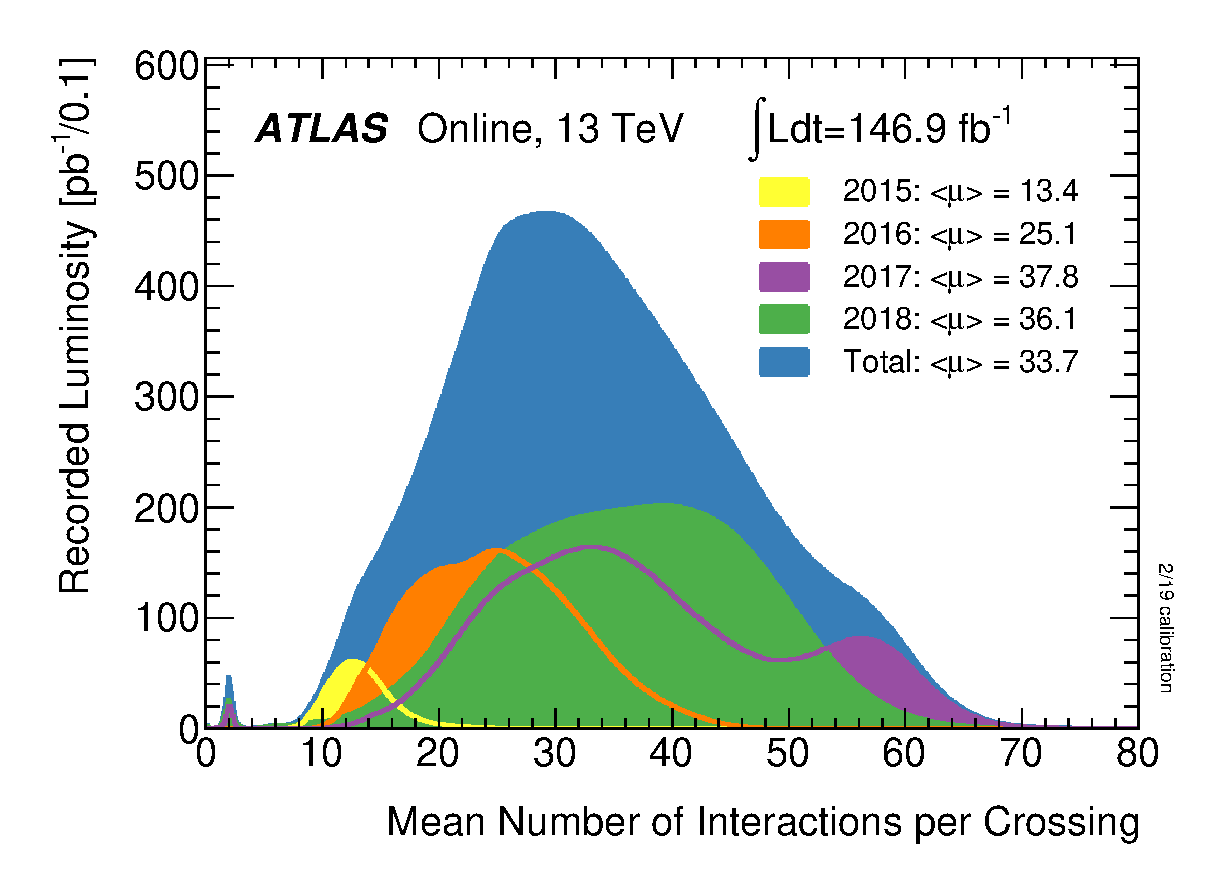
\includegraphics[width=0.55\linewidth]{Pictures/mu_2015_2018.eps}
    \caption{The luminosity-weighted distribution of the mean number of interactions per crossing is shown for Run-2 pp collision data. }
    \label{fig:mu_profile}
\end{figure}

Events are only used if all relevant detector components are operating normally. These events are part of the standard ``All Good'' Good Run List comprising a rotal integrated luminosity of $139$fb$^{-1}$ and data quality efficiency of $91.5$\%.

Throughout Run-2 the instaneous luminosity and so pile-up changed dramatically. This is accounted for in our MC modelling, as described in the next section.

%%%%%%%%%%%%%%%%%%%%%%%%%%%%%%%%%%%%
\subsection{Monte Carlo samples}
%This analysis uses samples reconstructed using release 21.0.  Derivations of MC samples were produced with the tags \texttt{p3654}, \texttt{p3652} which use \texttt{AthDerivation 21.2.44}.
%Derivations of data samples were made the tag \texttt{p3653} using \texttt{AthDerivation 21.2.44}. The samples are further processed  using \texttt{AnalysisBase 21.2.68} for systematic computation.

%\textcolor{red}{Add alternative MC samples for signal and backgrounds}\\

Monte Carlo samples are generated to compare to data in order to test Standard Model predictions and search for excesses. These simulations are also used to optimize the analysis before applying these techniques to our dataset. Monte Carlo events are fully simulated using the ATLAS detector simulation in the GEANT4 framework \cite{GEANT4} and reconstructed with standard ATLAS reconstruction software. Pile-up is simulated as additional $pp$ interations in a separate simulation step during digitization where minimum bias events are superimposed on the simulated signal events. These additional events are added based on that years recorded pile-up to account for dataset differences. 

Separate programs are used to generate the hard scattering process and to model the parton showering (PS), hadronization, and the underlying event (UE). The next sections summarize the simulation techniques for our signal vector boson fusion samples, other Higgs production modes, and relevant backgrounds.   

%\HERWIG~\cite{herwig} is used for PS and hadronisation in estimating systematic uncertainties with UE being modelled with \JIMMY~\cite{jimmy}.

%The CT10 and NNPDF3.0 parton distributions function (PDF) sets~\cite{Lai:2010vv}~\textcolor{red}{[missing NNPDF3.0 ref]} are used for the hard scattering process in \textsc{ Powheg-Box} v2~\cite{Nason:2009ai} ~\textcolor{red}{[unclear sinec 2 PDF sets are listed, are they used in different processes?]} while for \MADGRAPH5 (version 2.2.1 and 2.2.2)~\cite{Alwall:2014hca} the NNPDF23LO~\cite{Ball:2012cx} PDF set is used.
%The AZNLO~\cite{Aad:2014xaa} tune is used for the diboson and signal processes while the A14 tune~\cite{ATL-PHYS-PUB-2014-021} for other processes.
%The CTEQ6L1~\cite{Nadolsky:2008zw} PDF set is used for the \PYTHIA8 showering,
%with the NNPDF 3.0tune when interfaced to \textsc{ Powheg-Box} v2 and
%with the A14~\cite{ATL-PHYS-PUB-2014-021} tune when interfaced to \MADGRAPH5.

%The hard scattering NLO predictions from \SHERPA 2.2.1~\cite{Gleisberg:2008ta} are calculated using NNPDF 3.0 NNLO PDF set in conjunction with a dedicated set of tuned parameters from the parton shower developed by the \SHERPA authors~\cite{Schumann:2007mg}.

%The complete list of the MC samples and their configuration can be found in Appendix \ref{sec:append_samples}.
The fullset of data is split into three time-based categories. Data-taking conditions in 2015 and 2016 are averaged and described together as mc16a. 2017 and 2018 data-taking conditions are considered separately as mc16d and mc16e respectively. 

%%%%%%%%%%%%%%%%%%%%%%%%%%%%%%%%%%%%%%%%%%%%%%%%%%%%%%
\subsubsection{Vector boson fusion Higgs samples}

VBF Higgs events are generated through \textsc{POWHEG} \cite{Nason:2009ai} interfaced with \textsc{Pythia} 8 with the PDF4LHC15 parton distribution function (PDF) set \cite{PDF4LHC15}. Cross sections are calculated with full NLO QCD and EW corrections \cite{CiccoliniDennerDittmaier2007,Arnold2009} with an approximate NNLO QCD correction applied~\cite{Bolzoni2010}. These cross-sections as well as associated branching ratios are calculated by the LHC Higgs Cross Section Working Group Yellow Report 4 \cite{deFlorian:2016spz}. Generated events are normalized to calculated cross-sections. %Two tables below show first the production cross sections used to normalize the Higgs MC samples (including those for VBF) \ref{tab:MCSignal} and next summaries of the MC samples used including nominal production as well as alternative productions for the estimation of theoretical systematics, which are discussed further in the next chapter \ref{tab:samples}.  
%%%%%%%%%%%%%%%%%%%%%%%%%%%%%%%%%%%%%%%%%%%%%%%%%%%%%%
\subsubsection{Other production mode Higgs samples}

%\begin{table*}[tb]
% \centering
% \caption{SM Higgs boson production cross sections ($\sigma$) for gluon fusion, vector-boson fusion and associated production with a $W$ or $Z$ boson or with a $b\bar{b}$ or $t\bar{t}$ pair in $pp$ collisions at $\sqrt{s}=13$ TeV. First and second uncertainties represent theoretical systematic uncertainties calculated by adding in quadrature the QCD scale and PDF$+\alpha_s$ uncertainties, respectively. The last column shows the decay branching ratio ($B$) for $H \rightarrow \ell\nu\ell\nu$ with $\ell = e, \mu$.\label{tab:MCSignal}}
% \vspace{0.1cm}
% \begin{tabular}{ccccccc}
%   \hline \hline
%   \noalign{\vspace{0.05cm}}
%   $m_{H}$       & $\sigma\left(gg\to H\right)$ & $\sigma\left(qq'\to Hqq'\right)$ & $\sigma\left(q\bar{q}\to WH\right)$ & $\sigma\left(pp\to ZH\right)$   \\
%   $[{GeV}]$ & $[{\textrm{pb}}]$                 & $[{\textrm{pb}}]$                     &  $[{\textrm{pb}}]$                       & $[{\textrm{pb}}]$                    \\
%   \noalign{\vspace{0.05cm}}
%   \hline\hline
%   \noalign{\vspace{0.05cm}}
% TODO: take the gaussian errors instead of flat for ggF N3LO as recommended?
   
%   $125.0$\rule[-1mm]{0mm}{4.7mm} & $48.58$  $^{+4.6\%}_{-6.7\%}$ $^{+3.2\%}_{-3.2\%}$ & $3.782$  $^{+0.4\%}_{-0.3\%}$ $^{+2.1\%}_{-2.1\%}$ & $1.373$  $^{+0.5\%}_{-0.7\%}$ $^{+1.9\%}_{-1.9\%}$  
%                                  & $0.8839$ $^{+3.8\%}_{-3.1\%}$ $^{+1.6\%}_{-1.6\%}$ \\
%  
%   \noalign{\vspace{0.05cm}}
%   \hline\hline 
%   \noalign{\vspace{0.05cm}}
%   $m_{H}$       & $\sigma\left(gg\to ZH\right)$ & $\sigma\left(q\bar{q}/gg\to t\bar{t}H\right)$ & $\sigma\left(q\bar{q}/gg\to b\bar{b}H\right)$ & $B$  \\ 
%   $[{GeV}]$ & $[{\textrm{pb}}]$                  & $[{\textrm{pb}}]$                                  & $[{\textrm{pb}}]$                                 & $[10^{-3}]$\\
%   \noalign{\vspace{0.05cm}}
%   \hline\hline
%   \noalign{\vspace{0.05cm}}
%   $125.0$\rule[-1mm]{0mm}{4.7mm} & $0.1227$ $^{+25.1\%}_{-18.9\%}$ $^{+2.4\%}_{-2.4\%}$ & $0.5071$ $^{+5.8\%}_{-9.2\%}$ $^{+3.6\%}_{-3.6\%}$ & $0.4880$ $^{+20.2\%}_{-23.9\%}$ & $0.1240$ $\pm2.18\%$ \\
%  \noalign{\vspace{0.05cm}}
%  \hline\hline
%\end{tabular}
%end{table*}  

Other Higgs production modes gluon fusion (ggF), associated Higgs boson production ($VH$, $V=W,Z$) and Higgs boson production in association with a heavy quark pair ($ttH$, $bbH$) are important backgrounds in this analysis.% and listed in table \ref{tab:samples}.  

Similar to the VBF Higgs sample, ggF, $VH$, $ttH$ and $bbH$ are produced with \textsc{Pythia8}\cite{pythia,Sjostrand:2007gs} for decay, parton shower, hadronisation and multiple parton interactions.

%\begin{table}[tb]
%\caption{MC samples used to simulate Higgs boson production, including generators, QCD calculation accuracy and PDF sets.}
%\label{tab:samples}
%\centering
%\begin{tabular}{ llll}
%  \hline
%  \hline
%  Process & Generator & Accuracy in QCD & PDF set   \\
%  \hline
%   VBF & \textsc{Powheg-Box} v2~\cite{powheg1,powheg2,powheg3,powheg5}  & NLO & PDF4LHC~\cite{Butterworth:2015oua} \\
% \hline 
%  ggF & \textsc{Powheg-Box} v2 (NNLOPS)~\cite{powheg1,powheg2,powheg3,Campbell:2012am} & NNLO in $y^{H}$~\cite{Hamilton:2013fea}, & PDF4LHC~\cite{Butterworth:2015oua}  \\
%  & & $p_{T}^{H}$ consistent with \textsc{HqT}  & \\
%  & & (NNLO+NNLL)~\cite{Bozzi:2005wk,deFlorian:2011xf} & \\  
%  $VH$ & \textsc{Powheg-Box} v2 (\textsc{MiNLO})~\cite{powheg1,powheg2,powheg3,Luisoni:2013kna} & NLO & PDF4LHC~\cite{Butterworth:2015oua} \\
%  $tH$ & \textsc{Powheg-Pythia8} & NLO & PDF4LHC~\cite{Butterworth:2015oua} \\
%  $ttH$ & \textsc{Powheg-Box} v2~\cite{powheg1,powheg2,powheg3,powheg5} & NLO & PDF4LHC~\cite{Butterworth:2015oua} \\
%  $bbH$ & \textsc{Madgraph5\_aMC@NLO} (v.2.3.3)~\cite{Alwall:2014hca,Wiesemann:2014ioa} & NLO & NNPDF23~\cite{Ball:2012cx} \\
%\hline
%\hline
%\end{tabular}
%\end{table}
 
%%%%%%%%%%%%%%%%%%%%%%%%%%%%%%%%%%%%%%%
\subsubsection{Background samples}
\label{sec:bkgMC}

%%\begin{table}[h]
%  \centering
%  \caption{Listed MC generators that model signal and background processes with corresponding cross sections.}
%%  \scalebox{0.75}{
%{\footnotesize
%  \begin{tabular}{llrcc}
%    \hline\hline
%    Process & Generator & \hspace*{-3mm}$\sigma\cdot\mathrm{Br}$ (pb) & Precision $\sigma_{\mathrm{incl.}}$\\
%\hline 
%%VBF $H\rightarrow WW$  & \POWHEG+\PythiaEight & 0.808 & NNLO \\
%%    \hline
%%%    ggF $H\rightarrow WW $  & \POWHEG+\PythiaEight & 10.4 & NNLO+NNLL \\
%%    ggF $H\rightarrow WW $  & \POWHEG NNLOPS & 10.4 & NNLO+NNLL \\
%    $WH$ $H\rightarrow WW $ & \POWHEG+\PythiaEight (MINLO) & 0.293  & NNLO \\ % TO  BE checked
%    $ZH$ $H\rightarrow WW $ & \POWHEG+\PythiaEight (MINLO) & 0.189  & NNLO \\ % TO  BE checked
%   \red{ttH, tH, and bbH}
%    \hline 
%    \hline
%    $q\bar{q}/g\rightarrow WW \rightarrow \ell\nu\ell\nu$              & \textsc{SHERPA} 2.2.2 & 49.74  & NLO\\ 
%    $Z^{(\ast)}Z^{(\ast)} \to 2\ell2\nu~(m_{\ell\ell} \ge 4 )$GeV   & \textsc{SHERPA}  2.1  & 6.53   & NLO\\
%
%    $gg \to  2\ell2\nu$                     & \textsc{SHERPA}  2.1 & 0.87 & NLO\\
%
%    $q\bar{q}/g \to  \ell\nu\ell\ell$       & \textsc{SHERPA} 2.1 & 11.9 & NLO\\
%
%    $q\bar{q}/g, gg \to  \ell\ell\ell\ell$  & \textsc{SHERPA} 2.1 & 11.5 & NLO\\
%
%
%    EW $WW + 2$ jets $(\ell\nu\ell\nu)$   & \textsc{SHERPA} 2.1 & 0.012 & LO \\
%    EW $WZ + 2$ jets $(\ell\nu\ell\ell)$  & \textsc{SHERPA} 2.1 & 0.038 & LO \\
%    EW $ZZ + 2$ jets $(\ell\ell\ell\ell)$ & \textsc{SHERPA} 2.1 & 0.116 & LO \\
%    EW $q\bar{q} {\to}(Z\rightarrow\tau\tau) q\bar{q}$ & \textsc{SHERPA} & 2.54 & LO\\
%    \hline
%     inclusive $Z/\gamma^{\star} \to \ell\ell~(40 \ge m_{\ell\ell} \ge 10)$GeV & \textsc{SHERPA} 2.2.1 & $6.80 \times 10^{3}$ & NNLO\\ %%UPdate XS
%    inclusive $Z/\gamma^{\star} \to \ell\ell~( m_{\ell\ell} \ge 40)$ GeV       & \textsc{SHERPA} 2.2.1 & $2.107 \times 10^{3}$ & NNLO\\
%
   % $(W \to \ell\nu)\gamma~(p_{T}^{\gamma} > 7 )$GeV                 & \textsc{SHERPA} 2.2.2& 453 & NLO\\
%    $(Z \to \ell\ell)\gamma~(p_{T}^{\gamma} > 7 )$GeV                & \textsc{SHERPA} 2.2.2& 175 & NLO\\
%
%    $t\bar{t}$ di-leptonic($e,\mu ,\tau$)         & \textsc{Pythia 8} & 87.6 & NNLO+NNLL & \\
%    $Wt$ leptonic             & \textsc{POWHEG}+\textsc{Pythia 6} & 7.55 &  NLO & \\
%     \hline\hline
%  \end{tabular}
%  }
%  \label{tab:mcsamples}
%\end{table}

Main Standard Model backgrounds include events from production of dibosons, top-quark, $Z$+jets, $W$+jets and multijets. %They are summarised in Tab.~\ref{tab:mcsamples}. 

The $WW$ samples are generated using \textsc{SHERPA} 2.2.2 interfaced with NNPDF3.0 NNLO PDFs further described in \cite{Cascioli:2013gfa}. 
%They are generated at NLO with 0 and 1 jets and at LO accuracy with 2 and 3 jets. The production also requires $m_{\ell\ell}>4$ GeV, $p_T^{l1}>5$ GeV and $p_T^{l2}>5$ GeV. Loop-induced $gg$-initiated diboson processes are simulated by \textsc{SHERPA} 2.1.1 with zero or one additional jets, as described in \cite{Cascioli:2013gfa}. For $WW$ the sample is normalized to the NLO $gg\rightarrow WW$ cross section calculated in \cite{Caola:2015rqy} at $13$TeV so a k-factor of 2.3 applied to the sample.
%AT: For all other processes the cross sections are taken from the generator and are at LO. 

%For $q\bar{q}/g{\to}Z^{(\ast)}Z^{(\ast)}{\to}\ell\nu\ell\nu$ by \textsc{POWHEG} v2 a cut on the invariant mass of the two charged lepton $m_{\ell\ell} > 4 ~$GeV is required. In addition it is required that at least two charged leptons must have $p_T > 5 ~$GeV. The $ZZ$ is also simulated with \textsc{SHERPA} 2.1, as alternative sample. The $WZ$ is generated with \textsc{SHERPA} 2.1, using the CT10 PDFs, at NLO accurary for 0 and 1 jet and LO for 2 and 3. These samples include also the $\gamma*$ process and are produced with cuts on $m_{\ell\ell}>2 \times m_{l}+250$ MeV, $p_T^{l1}>5$ GeV, $p_T^{l2}>5$ GeV.

%The $ZZ$ is also simulated with \SHERPA 2.1.
%For the $W$+jets estimation, which will be described in Section~\ref{sec:FakeEstimation}, 
%all the diboson process, except for $gg\to ZZ$, are simulated with \OWHEG+\PythiaEight.

%Diboson samples are generated using \SHERPA 2.2.1 interfaced with NNPDF 3.0 NNLO PDFs and normalised to cross sections calculated at NLO\cite{CampbellEllis2010}.
%%%% EW samples  
%The \textsc{SHERPA} 2.1.1 MC is used for the modeling of diboson process with no $O(\alpha_S)$ terms for the $\ell\ell\ell\ell, \ell\nu\ell\ell$ and $\ell\nu\ell\nu$ plus two jets final states as well as the $q\bar{q}{\to}Zq\bar{q}$ processes with a requirement of $Z{\to}\tau\tau$ ($m_{\tau\tau} > 40$GeV) decay, which are also known as electroweak (EW) processes, at the LO accuracy.

$Z$+jets (or Drell-Yan) production is simulated with \textsc{SHERPA} 2.2.1 using the NNPDF3.0 NNLO PDFs with dedicated parton shower tuning developed by Sherpa authors. 
%In order to generate sufficient high V ($p_T$) statistics, V+jets samples are split according to max($H_T$, $p_T^V$). 
%Additionally, to obtain sufficient heavy-flavour final state statistics, the V+jets samples are generated applying filters.
%Moreover, for the $Z \to \tau \tau$ an additional filter on the leptons( or hadrons) $p_T$ has been added to better populate the analysis phase space.
%Five filtered regions have been defined, but only 2 are used in the analysis: lep13lep7, lep15had20.
%Only the first three max($H_T$, $p_T^V$) slices are available with these filters.
%Therefore, in the signal channel up to $140<$max($H_T$, $p_T^V$)$<280$ the lepton/had $p_T$ filtered samples are used instead for the high max($H_T$, $p_T^V$) slice the nominal samples are used.
%Samples are normalised using cross sections calculated at NNLO accuracy~\cite{MelnikovPetriello}.

Top-quark pair production (or $t\bar{t}$) is simulated using \textsc{POWHEG} with the \textsc{ Powheg-Box} framework using the NNPDF 3.0 PDFs and interfaced with \textsc{Pythia 8} using NNPDF 2.3 PDFs for parton showering. %, with A14 tune.
%The $t\bar{t}$ samples generated include a filter to require that the $W$ bosons decays leptonically. All the three leptons ($e, \mu, \tau$) are considered for the $W$ decay in \textsc{POWHEG}. The $\tau$s are then decayed by \textsc{Pythia 8} in either leptonically or hadronically mode.
%Samples are normalised using cross sections calculated at NNLO+NNLL~\cite{Czakon:2013}.

Single top, mainly $Wt$, production is generated with \textsc{Powheg-Box}\,2.0 interfaced to \textsc{Pythia} 6.428 for parton showering.
%\textsc{ EvtGen}\,1.2.0~\cite{Lange:2001uf} is used for properties of the bottom and charm hadron decays.
%The predicted $\ttbar$ production cross section is calculated with the \textsc{Top++2.0}
%program to NNLO in perturbative QCD, including soft-gluon resummation to 
%NNLL order (see~\cite{Czakon:2011xx} and references therein), and assuming a top-quark mass of 172.5 $\gev$.
%$Wt$ sample is required to have at least two charged leptons in the final state.
%Both $\ttbar$ and $Wt$ samples are required to have at least two charged leptons in the final state.

$Z\gamma$ and $W\gamma$ productions are modeled using \textsc{SHERPA} 2.2.2 at the NLO accuracy for 0- and 1-jet.
%For both $Z\gamma$ and $W\gamma$ processes the $p_T$ of the $\gamma$ are
%required to be larger than 7 GeV, and the distance in the $\eta - \phi$ plane
%$\Delta R = \sqrt{(\Delta \eta)^{2} + (\Delta \phi)^{2}} > 0.1$.
%In addition the leptons from $Z$ boson in the $Z\gamma$ final state is required to have $m_{\ell\ell} > 2 $GeV.

The $W$+jets process modeling is based on a data-driven method described in the next chapter. MC samples (with the same MC generators for both $W+$jets and $Z+$jets samples) are used to validate the fake estimation and estimate sample composition uncertainties. These processes are generated with \textsc{POWHEG} MiNLO interfaced to \textsc{Pythia 8} with the AZNLO tune. 
%The PDF set used in \textsc{POWHEG} is CT14nnlo whereas the PDF set used in the parton shower is the CTEQ6 L1 leading order set.
%The alternative V+jets samples have been produced using the LO matrix-element generator ALPGEN v2.14 interfaced to \textsc{Pythia 6} to model the parton shower. The parton-shower tune Perugia2011C and the CTEQ6L1 PDF set have been used. 
%Up to five additional partons are modelled by the matrix elements, merged with the MLM prescription with a matching scale of 20 GeV. 
%The predictions follow a four-flavour-number-scheme (4FNS) for the production of heavy-flavour jets.
%Other MC generators, like \SHERPA and \MadGraph, are availble h
%AT All simulated samples include the effect of pile-up from multiple interactions in the same and neighbouring bunch crossing. 
%AT This is achieved by overlaying minimum bias events, simulated using \PythiaEight, using A2 tune and interfaced with MSTW2008LO PDFs. 
%AT All samples are processed through the Geant-4 based ATLAS detector simulation, and reconstructed with the standard ATLAS reconstruction software

\section{Object definitions}
This analysis utilizes a number of calibrated physics objects and the accurate use of each determines the precision of our $H\rightarrow WW$ differential cross section measurement. Lepton, jet, and missing transverse energy reconstruction, isolation, and calibration were described in some detail in the previous chapter. This chapter focuses on the particular parameters applied for these physics objects in this analysis. The object definitions are used in accordance with the $H\rightarrow WW$ coupling analysis for consistency where optimization focussed on $H \rightarrow WW$ measurements at large. Finally, further observables used in event selection are defined and described here as well. 

\subsection{Lepton}

Our choice of lepton identification algorithm impacts both the rejection of fake lepton backgrounds ($W+$jets) and QCD background. Tighter requirements on lepton identification decrease signal efficiency so the optimal criteria balance high signal efficiency and high background rejection. Further studies on lepton identification and isolation criteria can be found in the HWW Coupling Support note \cite{HWWCoupling}.

Specific muon and electron requirements will be detailed next. Overall, all events must have at least two leptons tracks and each lepton track must have $p_T>400$MeV. Further, leptons all are required to originate at the hard-scatter primary vertex which is defined as the primary vertex with the largest track $\sum p_T$. Leptons must pass two impact parameter selections to ensure they originate at the primary vertex. The longitudinal impact parameter of each lepton track is defined as $|z_0\mathrm{sin}\theta|$ where $z_0$ is the impact paramter and $\theta$ the track angle. Each lepton longitudinal impact parameter must be less than 0.5mm. The significance of the transverse impact parameter is calculated with respect to the beam line ($|d_0|/\sigma_{d_0}$) and has a requirement of three (five) for muons (electrons) as recommended by the Muon and E/$\gamma$ combined performance groups. 

\subsubsection{Electron}
Electron identification utilizes energy deposits in the calorimeter and reconstructed tracks in the inner detector. An electron likelihood combines these quantities and sets recommended working points (\textit{Loose, Medium, Tight}) which correspond to increasing levels of background rejection. Further descriptions of the current $E/\gamma$ combined performance group recommendations and methods can be found here \cite{ATL-PHYS-PUB-2015-041}.

This analysis uses both the \textit{Medium} and \textit{Tight} identification selections which have 94\% and 88\% identification efficiency respectively for an electron with $E_T=100$ GeV. Electrons with $E_T>25$GeV must pass the \textit{Medium} identification while those with $15<E_T<25$GeV are required to pass the \textit{Tight} selection. This mimics the selection for the $H\rightarrow WW$ coupling analysis where optimization studies demonstrated its impact on overal significance. 

Electrons are identified in the range $|\eta|<2.47$, where the transition region between barrel and endcaps in the LAr calorimeter ($1.37<|\eta|<1.52$) is excluded.

Electron isolation uses two different selections based on electron track $p_T$. For $p_T>25$GeV the \textit{IsoGradient} working point is used. This requires calorimeter and track isolation about cones of $\Delta R =0.2$ (\textit{topoetcone20}, \textit{ptvarcone20}). Electron isolation is changed to the fixed cut track cone isolation for $p_T <25$GeV to further eliminate fake background contributions. These require both track and calorimeter variables to fall below the $p_T$ dependent $0.1143\times p_T + 92.14$. 

The following table summarizes electron selection criteria \ref{tab:ElecSelection}.

\begin{table}[h!]
  \centering
  \caption{Electron selections}
  \scalebox{0.9}{
  \begin{tabular}{llccll}
    \hline\hline
     $p_T$ range & $|\eta|$ range   & Electron ID & Isolation     & Impact parameter\\
    \hline\hline
      $< 25$GeV & \multirow{2}{*}{$0 - 1.37$, $1.52 - 2.47$}  & Tight           & FixedCutTrackCone40 & \multirow{2}{*}{$|z_0 \mathrm{ sin} \theta|<0.5$, $|d_0|/\sigma_{d_0}<5$} \\
      $> 25$GeV &                                                              & Medium          & IsoGradient            & \\
    \hline\hline 
  \end{tabular}}
  \label{tab:ElecSelection}
\end{table}

\subsubsection{Muon}

As described previously, muons can be reconstructed using inner detector tracks, calorimeter deposits, and muon spectrometer tracks. The muon combined performance group performs an overall fit using each of these physical quantites and recommends six muon identification working points- \textit{VeryLoose, Loose, Medium, Tight, High-pT, Low-pT}.  The combination is performed through an overall fit using the hits of the inner detector track, the energy loss in the calorimeter, and the hits of the track in the muon system. Muons in this analysis must fit the \textit{Tight} selection as well as pass cuts $p_T>15$GeV and $|\eta|<2.5$. Muon identification and isolation criteria match those used in the $H\rightarrow WW$ coupling analysis and optimize background rejection and signal efficiency. Muon isolation uses calorimeter and track isolation with a cone of $\Delta R=0.2$ (\textit{topoetcone20, ptvarcone20}). 
Muon selection criteria are summarized in the table below \ref{tab:MuonSelection}. 

\begin{table}[h]
  \centering
  \caption{Muon selections}
  \scalebox{0.9}{
  \begin{tabular}{llrccc}
    \hline\hline
     $p_T$ range   & $|\eta|$ range & Muon ID    & Calo Isolation           & Track Isolation             & Impact parameter\\
    \hline\hline
      $> 15$GeV & < 2.5  & ``Tight''  & $E_T^{cone20}/p_T<0.09$  & $p_T^{varcone30}/p_T<0.06$  & $|z_0 \mathrm{ sin} \theta|<0.5$, $|d_0|/\sigma_{d_0}<3$ \\
    \hline\hline
  \end{tabular}}
  \label{tab:MuonSelection}
\end{table}


%%%%%%%%%%%%%%%%%%%%%%%%%%%%%%%%%%
\subsection{Jets}

Jets constitute an important part of the analysis both in their number and characteristics. Our signal region selection and most control regions require at least two jets but in order to estimate and reject $ggF$ Higgs background events, regions with less than two jets are also studied. ``Tagging'' jets refer to those considered in our jet requirement though others may be defined. As detailed in the previous chapter, jets reconstruction uses the anti-$k_t$ algorithm to create jet tracks from calorimeter energy deposits within a cone of $R = 0.4$ and this analysis uses particle flow jet reconstruction.   

Jets are required to have $p_T > 30$GeV to eliminate high potential for pile-up jets in the full $\eta$ range, $|\eta| < 4.5$. ``Jet vertex tagger'' variables suppress pile-up events through combinations of multiple variables into a single jet tagger. For jets with $p_T < 60$GeV and $|\eta| < 2.4$, the JVT variable is required to be larger than 0.59. In the forward region a designated tagger called ``fJVT'' ought to be applied. However, the current analysis leaves out this requirement leading to more jet pile-up than expected. 

The VBF signal region contains an additional jet observable, central jet veto (CJV), which cuts on events with additional jets (other than the two ``tagged'' jets) which have $p_T>20$GeV within the rapidity gap between two leading jets. These increase VBF sensitivity through removal of hadronic backgrounds.
%%%%%%%%
\subsubsection{$b$-tagged jet}

The Jet/$E_T^{miss}$ group recommends tools to identify jets formed from bottom quarks. While the previous HWW analysis used the MV2C10 jet tagging algorithm, the current analysis utilizes the DL1 tagger. Both tools use jet kinematics, impact parameters, and secondary vertex variables as input to machine learning classifiers. The DL1 tagger uses a neural network training method (the MV2C10 a boosted decision tree) trained with $t\bar{t}$ signal to discriminate $b$-quarks from light and $c$-quarks. The DL1 tagger shows greater b-veto efficiency in isolating top background events and so is used in this analysis. This optimization follows that performed for the HWW coupling measurement \cite{HWWCoupling}. 

%%%%%%%%%%%%%%%%%%%%%%%%%%%%%%%%%
\subsection{Missing transverse energy}

Missing transverse energy is used to both suppress background and build other variables used in signal selection like $m_{tt}$ and $p_T^{tot}$. $E_T^{miss}$ definitions and calculation is explained in the previous chapter. This analysis uses the ``Tight'' $E_T^{miss}$ working point which has proven the most robust against increasing pile-up.

%%%%%%%%%%%%%%%%%%%%%%%%%%%%%%%%%
\subsection{Overlap removal}
Overlap removal is applied to electrons, muons, and jets following current recommendations and using the official ASG tool \cite{Twiki_ASG}. Current removal steps can be summarized as followed based upon \cite{ORpresc,ORpresc_1}:
\begin{itemize}
\item If a muon and electron share an ID track the electron is removed and if a calo-tagged muon shares an ID track with an electron, the muon is removed.
\item If $\Delta$ R(jet, e) $< 0.2$ the jet is removed (to eliminate overlap with the nearby electron). The electron is removed if $\Delta$ R(jet, e) < min(0.4, 0.04 + 10 GeV/$p_T^e$).
\item If $\Delta$ R(jet, $\mu$) $< 0.2$ and the jet has less than three associated tracks with $p_T>500$MeV the jet is removed. The jet is also removed if the $p_T$ ratio of the muon and jet is larger than 0.5 and the ratio of the muon $p_T$ and the sum of the $p_T$ of all jet tracks with $p_T>500$GeV is larger than 0.7. The muon is removed if $\Delta$ R(jet, $\mu$) < min(0.4, 0.04 + 10 GeV/$p_\mathrm{{T}}^{\mu}$) for any surviving jets.
%\item Jets are discarded if they are within a cone of size $\Delta R < 0.2$ of an electron candidate, or if they have less than three associated tracks and are within a cone of size $\Delta R < 0.2$ of a muon candidate. However, if a jet with three or more associated tracks is within a cone of size $\Delta R < 0.4$ of a muon candidate, or any jet is within $0.2 < \Delta R < 0.4$ of an electron candidate, the corresponding electron or muon candidate is discarded. 
\end{itemize}


%%%%%%%%%%%%%%%%%%%%%%%%%%%%%%%%%%%%%%%%%%%%%%%%
\section{Common Observables}

Dedicated observables are used in this analysis to reject and isolate backgrounds as well as to enhance VBF signal strength. This section lists and describe key observables used in the analysis.

\begin{itemize}
\item $m_{\tau \tau}$: This can be defined as in the previous chapter's $E_T^{miss}$ section, if charged leptons are the products of a pair of $\tau$ leptons, the neutrinos are collinear with the charged leptons, and the neutrinos are the only source of the observed $E_\mathrm{{T}}^{miss}$ in the event. We cut on this variable to suppress $Z\rightarrow\tau\tau$  events. 
\item $N_{b-jet}$: Defines number of jets with $p_T >20$ GeV identified as b-jets from the b-tagged algorithm (DL1) and used to reject $t\bar{t}$ background.
\item $p_\mathrm{{T}}^{ll}$: Topological variable ransverse momentum of the dilepton system. This cut targets Drell-Yan/$Z\rightarrow\tau\tau$ events through a cut at 70 GeV. 
\item $\Delta \phi_{ll}$: The two leptons from HWW decays tend to be collimated especially compared to non-resonant WW backgrounds. This is due to the spin-zero initial state of the resonant process. 
\item $m_{ll}$: The invariant mass of the two leptons from the hard scattering interaction. Similar to $p_T^{ll}$, targets Drell Yan events and is cut on at 70GeV in the control region.
\item $m_\mathrm{{T}}$: Transverse mass is used as discriminant variable though not directly cut. Defined as
\begin{equation}
m_\mathrm{{T}} = \sqrt{ {(E_{ll} + E_\mathrm{{T}}^{miss})}^2 - {|p_{ll} + E_\mathrm{{T}}^{miss}|}^2 }
\end{equation}
  where $E_{ll} = \sqrt{|p_{ll}|^2 + m_{ll}^2 }$ .
\item $p_T^\mathrm{tot}$:
Total transverse momentum $p_T^\mathrm{tot}$, defined in the targeted $E_T^{miss}$ chapter. Aids in rejecting events with significant soft gluon radiation but not high $p_T$ jets.
\item  $\Delta Y_{jj}$: VBF Higgs signal events are characterized by a large separation of the two tagging jets in rapidity. This variable is used as a signal region cut. 
\item $m_{jj}$:
VBF Higgs events end to have a high jet invariant mass ($m_{jj}$), defined by combining mass of tagged jets. This analysis applies a cut on $m_{jj}$ in our signal region. 
\item $\eta_{lep}$ centrality: This analysis uses an outside lepton veto defined to reject events with leptons outside the rapidity gap between the two tag jets. This OLV variable is defined using $\eta$ of the tagged jets and leptons as follows:
\begin{eqnarray}
&& \textrm{OLV}_{l_0} = 2 \cdot |\frac{\eta_{l_0}-\bar{\eta}}{\eta_{j_0}-\eta_{j_1}}|  \nonumber\\
&& \textrm{OLV}_{l_1} = 2 \cdot |\frac{\eta_{l_1}-\bar{\eta}}{\eta_{j_0}-\eta_{j_1}}|  \nonumber\\
&&\nonumber \\
&& \eta_{\mathrm{lep}} \, \textrm{centrality} = \textrm{OLV}_{l_0} + \textrm{OLV}_{l_1}
\label{eqn:contOLV_def}
\end{eqnarray}
where $\bar{\eta} = (\eta_{j_0} + \eta_{j_1})/2$ and so for each lepton: 
 \begin{equation}
   \textrm{OLV}_l \left\{
   \begin{array} {ll}
     = 0 & \quad \textrm{:  the lepton is right in the middle of the rapidity gap between the two tag jets.} \\
     < 1 & \quad \textrm{:  the lepton lies within the rapidity gap between the two tag jets.} \\
     >1  & \quad \textrm{:   the lepton is outside the rapidity gap between the two tag jets.} 
    \end{array} \right. 
 \end{equation}
\item $\mathrm{\sum_{l,j} M_{lj}}$: The sum of the invariant masses of all possible lepton-jet pairs are used to train our signal discriminant as VBF Higgs signal peaks at a higher value than the dominant backgrounds. VBF signal jets tend to be very forward while lepton central so a large separation between lepton and jets is expected as opposed to typical background topologies. 
\end{itemize}


\section{Event selection}
Figure \ref{fig:FeynmanDiagram} shows the Feynman diagram for the vector boson fusion Higgs production mode. Two energetic jets with large separation in rapidity accompany the Higgs and its decay products. In addition, since the Higgs is created through the fusion of two electro-weak bosons, there is no QCD interaction between the jets and the Higgs boson or its decay products. The main backgrounds this analysis seeks to mitigate include top quark production, Drell-Yan/$Z$, di-bosons ($WW$, $WZ$, $ZZ$, and $W\gamma$), gluon-gluon fusion (ggF) Higgs production, and $W$+jets. 

\begin{figure}[!htbp]
    \centering
    \includegraphics[width=0.2\linewidth]{Pictures/fig_01b_2.pdf}
    \caption{Feynman diagram for VBF Higgs production}
    \label{fig:FeynmanDiagram}
\end{figure}

This analysis controls and estimates these backgrounds with a variety of methods depending on characteristics of each background. Major backgrounds are estimated in CRs and minor backgrounds are estimated using MC simuation. Top quark production is suppressed in the SR by a $b$jet veto requirement, and can be studied in a very pure orthogonal set of bins in the signal region defined by a boosted decision tree discriminant. A pure validation region is also defined to cross-check top MC modelling. The Drell-Yan/$Z$ background is suppressed by kinematic requirements and is constrained in a dedicated and orthogonal CR and ultimately normalized in the signal phase space. The $ggF$ Higgs produciton mode is particularly difficult to separate from the VBF production mode, therefore several CRs are defined to constrain it in data, and ultimately its normalization is determined in the signal phase space. The $W$+jets background is estimated with data-driven techniques, as described in the next chapter's section on fake estimation, and then fixed in the simultaneous fit of SR and CRs.

The analysis employs multivariate analysis (MVA), more specifically 2D boosted decision trees trained to discriminate between samples. Specfically there are six trained BDTs used to separate: $WW+$top and $VBF$ events, ggF events from all other samples in each of their three control regions, $WW+$top events and VBF, and $WW$ and top events from one another. The use of these BDTs separates the backgrounds from our signal in the signal region and maintains discrimination between the two $WW$ and top background samples. The  $WW+$top vs. $VBF$ BDT is discussed in this section while the others are explained within in the next dedicated background chapter. In addition, two other types of BDT have been tested in this analysis: a $Z+$jets vs. VBF BDT and a 3D BDT to separate $ggF$, $WW$ and VBF events. Results from these tests showed that though these led to minimization of background (in the case of $Z+$jets vs. VBF) and good discrimination between key backgrounds in the signal region (in the case of the 3D BDT), when used in the final fit with systematic uncertainties they showed no significant decrease in calculated error in the VBF coupling value. Results from these studies are shown in the Appendix. 

\begin{table}[h!]
\centering
\scalebox{0.8}{
\begin{tabular}{|l|c|c|c|c|c|}
\hline
\multirow{2}{*}{Background}   & Relative size  & Relative size  & \multirow{2}{*}{Estimation}  & \multirow{2}{*}{{Generator}} \\
                              & Pre-selection  & Signal Region  &                       & \\
\hline                                                         
$WW$                       & $\sim 8\%$               & $\sim20\%$    & MC only + BDT           & \textsc{SHERPA} 2.2.2 ($gg \rightarrow WW$: \textsc{SHERPA} 2.1)\\
Top		              & $\sim 73\%$   	       &  $\sim61\%$     & Data+MC (Top CR)      & \textsc{POWHEG}+\textsc{Pythia} 8\\
$ggF$ Higgs                     & $< 1\%$    	       &  $\sim2\%$     & MC only + BDT           & \textsc{POWHEG}+\textsc{Pythia} 8 NNLOPS\\
$W$+jets                        & $\sim2.5\%$ 		& $\sim4\%$ 	& Data-driven           & - \\
$Z\rightarrow \tau\tau$                          & $\sim16\%$	       & $\sim7\%$		& Data+MC ($Z\rightarrow \tau\tau$ CR)     & \textsc{SHERPA} 2.2.1 \\
$W\gamma$,$W\gamma^{*}$       & $\sim1\%$		&  $\sim2.5\%$    & MC only               & \textsc{SHERPA} 2.1/\textsc{SHERPA} 2.2.2 \\
\hline
\end{tabular}
}
\caption{Each background and its relative size of in SR (after all cuts), estimation method, and generator.}
\label{tab:bkgsum}
\end{table}

\subsection{Pre-selection}
The VBF differential analysis shares object definitions with the VBF and ggF coupling analysis and pre-selection cuts are based off of those used in the 2016 ggF and VBF $H\rightarrow WW$ 36.1fb$^{-1}$ cross-section paper \cite{Aad:1975394}. The VBF selection utilizes observables defined in the previous section. Cuts applied in the preselection region are listed and described in the table below. 
\begin{table}[h!]
\centering
\small{
\begin{tabular}{|l|c|c|c|c|c|}
\hline
\multirow{2}{*}{Pre-sel cut}   & Description \\
				&	 \\
\hline
Channel Selection	& Fits $e\mu$/$\mu e$ channel/event weight applied\\  
Trigger Selection	&  Trigger selected \\
Trigger Matching	&  Trigger weight applied  \\
Data driven muon/electron & W+jets split into electron and muon fake flavors \\
Cut Jet Cleaning	& Pass loose jet cleaning \\
Cut $V\gamma$/$Z+$jets overlap & Eliminate any $Z+$jets events that overlap with $V\gamma$ \\ 
Only two leptons       	&  Require exactly 2 leptons (in case of fakes make sure 1 ID/1 Anti-ID) \\
Lead lepton $p_T$	& $p_T^{lead} > 22 $GeV \\
Sublead lepton $p_T$	& $p_T^{sublead} >15 $GeV \\
Opposite sign leptons	&  Require zero dilepton charge \\
$m_{ll}$ selection cut	&  $m_{ll} > 10$GeV \\
Fake Factor	& W+jets weight applied \\
\hline
\end{tabular}
\caption{Table describing pre-selection cuts applied in common with VBF and $ggF$ coupling analyses}
\label{tab:preseldef}
}
\end{table}

Yields for all samples as well as data for pre-selection cuts are shown in the following table.
\begin{table}[h!]
\scalebox{.35}{
%%% created on Sat Apr 18 17:21:56 2020 from TQSampleFolder 'samples' with TQLibrary UNKNOWN compiled with GCC 8.3.0 against ROOT 6.16/00
\providecommand{\xmark}{{\sffamily \bfseries X}}
\providecommand\rotatecell[2]{\rotatebox[origin=c]{#1}{#2}}
\begin{tabular}{ r || r  r | r  r || r  r  r | r  r  r  r }
\ensuremath{\sqrt{s}=13 TeV}, \ensuremath{\mathcal{L}=139 fb^{-1}}  (Full~Run~2) & $H_{VBF}$ & $H_{ggF}$ & $WW$ & Other VV & Top & Zjets & Mis-Id & Total Bkg & Significance & Data & Data/MC\tabularnewline
\hline
Channel Selection & \ensuremath{904.81\pm 0.92} & \ensuremath{9240.38\pm 10.13} & \ensuremath{175857.28\pm 140.42} & \ensuremath{22386.99\pm 78.25} & \ensuremath{1709307.70\pm 287.98} & \ensuremath{655027.79\pm 1233.45} & \ensuremath{5008168.16\pm 4730.67} & \ensuremath{7579988.31\pm 4899.95} & \ensuremath{0.33\pm 0.00} & \ensuremath{4374979} & \ensuremath{0.58\pm 0.00}\tabularnewline
Trigger Selection & \ensuremath{904.81\pm 0.92} & \ensuremath{9240.38\pm 10.13} & \ensuremath{175857.28\pm 140.42} & \ensuremath{22386.99\pm 78.25} & \ensuremath{1709307.70\pm 287.98} & \ensuremath{655027.79\pm 1233.45} & \ensuremath{5008168.16\pm 4730.67} & \ensuremath{7579988.31\pm 4899.95} & \ensuremath{0.33\pm 0.00} & \ensuremath{4374979} & \ensuremath{0.58\pm 0.00}\tabularnewline
Trigger Matching & \ensuremath{882.26\pm 0.90} & \ensuremath{8940.07\pm 9.82} & \ensuremath{173094.52\pm 138.41} & \ensuremath{21501.64\pm 77.38} & \ensuremath{1678206.02\pm 283.57} & \ensuremath{624251.33\pm 1168.16} & \ensuremath{5151805.35\pm 4644.01} & \ensuremath{7657798.93\pm 4799.69} & \ensuremath{0.32\pm 0.00} & \ensuremath{4352644} & \ensuremath{0.57\pm 0.00}\tabularnewline
W+jets flavour split muon & \ensuremath{882.26\pm 0.90} & \ensuremath{8940.07\pm 9.82} & \ensuremath{173094.52\pm 138.41} & \ensuremath{21501.64\pm 77.38} & \ensuremath{1678206.02\pm 283.57} & \ensuremath{624251.33\pm 1168.16} & \ensuremath{4675498.22\pm 4228.78} & \ensuremath{7181491.80\pm 4399.19} & \ensuremath{0.33\pm 0.00} & \ensuremath{4352644} & \ensuremath{0.61\pm 0.00}\tabularnewline
W+jets flavour split electron & \ensuremath{882.26\pm 0.90} & \ensuremath{8940.07\pm 9.82} & \ensuremath{173094.52\pm 138.41} & \ensuremath{21501.64\pm 77.38} & \ensuremath{1678206.02\pm 283.57} & \ensuremath{624251.33\pm 1168.16} & \ensuremath{3625576.16\pm 3693.41} & \ensuremath{6131569.74\pm 3887.35} & \ensuremath{0.36\pm 0.00} & \ensuremath{4352644} & \ensuremath{0.71\pm 0.00}\tabularnewline
Jet Cleaning & \ensuremath{882.26\pm 0.90} & \ensuremath{8940.07\pm 9.82} & \ensuremath{173094.52\pm 138.41} & \ensuremath{21501.64\pm 77.38} & \ensuremath{1678206.02\pm 283.57} & \ensuremath{624251.33\pm 1168.16} & \ensuremath{3625576.16\pm 3693.41} & \ensuremath{6131569.74\pm 3887.35} & \ensuremath{0.36\pm 0.00} & \ensuremath{4352644} & \ensuremath{0.71\pm 0.00}\tabularnewline
Overlap: Vgamma/Vjets & \ensuremath{882.26\pm 0.90} & \ensuremath{8940.07\pm 9.82} & \ensuremath{173094.52\pm 138.41} & \ensuremath{21501.64\pm 77.38} & \ensuremath{1678206.02\pm 283.57} & \ensuremath{624251.33\pm 1168.16} & \ensuremath{3625576.16\pm 3693.41} & \ensuremath{6131569.74\pm 3887.35} & \ensuremath{0.36\pm 0.00} & \ensuremath{4352644} & \ensuremath{0.71\pm 0.00}\tabularnewline
Only two Leptons & \ensuremath{880.17\pm 0.89} & \ensuremath{8934.45\pm 9.82} & \ensuremath{172870.71\pm 138.36} & \ensuremath{20467.40\pm 77.14} & \ensuremath{1662432.27\pm 282.33} & \ensuremath{622191.46\pm 1160.36} & \ensuremath{3621793.98\pm 3681.91} & \ensuremath{6108690.27\pm 3873.99} & \ensuremath{0.36\pm 0.00} & \ensuremath{4331979} & \ensuremath{0.71\pm 0.00}\tabularnewline
$p_{t}^{lead} > 22$ GeV & \ensuremath{880.17\pm 0.89} & \ensuremath{8934.45\pm 9.82} & \ensuremath{172870.71\pm 138.36} & \ensuremath{20467.40\pm 77.14} & \ensuremath{1662432.27\pm 282.33} & \ensuremath{622191.46\pm 1160.36} & \ensuremath{3621793.98\pm 3681.91} & \ensuremath{6108690.27\pm 3873.99} & \ensuremath{0.36\pm 0.00} & \ensuremath{4331979} & \ensuremath{0.71\pm 0.00}\tabularnewline
$p_{t}^{\rm sublead} > 15$ & \ensuremath{879.98\pm 0.89} & \ensuremath{8933.88\pm 9.82} & \ensuremath{172854.38\pm 138.35} & \ensuremath{20409.32\pm 77.10} & \ensuremath{1661877.68\pm 282.29} & \ensuremath{622068.28\pm 1160.19} & \ensuremath{3620023.39\pm 3681.17} & \ensuremath{6106166.94\pm 3873.23} & \ensuremath{0.36\pm 0.00} & \ensuremath{4330240} & \ensuremath{0.71\pm 0.00}\tabularnewline
OS Leptons & \ensuremath{879.86\pm 0.89} & \ensuremath{8933.68\pm 9.82} & \ensuremath{172771.82\pm 134.49} & \ensuremath{20042.40\pm 38.48} & \ensuremath{1661388.47\pm 282.25} & \ensuremath{621966.33\pm 1160.06} & \ensuremath{3614469.54\pm 3678.75} & \ensuremath{6099572.24\pm 3870.18} & \ensuremath{0.36\pm 0.00} & \ensuremath{4326784} & \ensuremath{0.71\pm 0.00}\tabularnewline
$M_{\ell\ell} > 12/10$ GeV & \ensuremath{879.85\pm 0.89} & \ensuremath{8933.66\pm 9.82} & \ensuremath{172771.33\pm 134.49} & \ensuremath{20041.83\pm 38.48} & \ensuremath{1661368.39\pm 282.25} & \ensuremath{621964.49\pm 1160.06} & \ensuremath{3614188.72\pm 3678.68} & \ensuremath{6099268.41\pm 3870.11} & \ensuremath{0.36\pm 0.00} & \ensuremath{4326642} & \ensuremath{0.71\pm 0.00}\tabularnewline
SF: Z Veto & \ensuremath{879.85\pm 0.89} & \ensuremath{8933.66\pm 9.82} & \ensuremath{172771.33\pm 134.49} & \ensuremath{20041.83\pm 38.48} & \ensuremath{1661368.39\pm 282.25} & \ensuremath{621964.49\pm 1160.06} & \ensuremath{3614188.72\pm 3678.68} & \ensuremath{6099268.41\pm 3870.11} & \ensuremath{0.36\pm 0.00} & \ensuremath{4326642} & \ensuremath{0.71\pm 0.00}\tabularnewline
Leptons ID, singleFakes 1 anti-ID,1 ID, doubleFakes 2*anti-ID & \ensuremath{596.53\pm 0.74} & \ensuremath{5630.33\pm 7.80} & \ensuremath{126996.63\pm 115.72} & \ensuremath{11152.41\pm 25.92} & \ensuremath{1165160.56\pm 237.51} & \ensuremath{257221.77\pm 444.61} & \ensuremath{1150777.06\pm 1622.64} & \ensuremath{2716938.76\pm 1703.28} & \ensuremath{0.36\pm 0.00} & \ensuremath{1587474} & \ensuremath{0.58\pm 0.00}\tabularnewline
Apply QCD FF weight & \ensuremath{596.53\pm 0.74} & \ensuremath{5630.33\pm 7.80} & \ensuremath{126996.63\pm 115.72} & \ensuremath{11152.41\pm 25.92} & \ensuremath{1165160.56\pm 237.51} & \ensuremath{257221.77\pm 444.61} & \ensuremath{523146.10\pm 1291.33} & \ensuremath{2089307.80\pm 1391.31} & \ensuremath{0.41\pm 0.00} & \ensuremath{1587474} & \ensuremath{0.76\pm 0.00}\tabularnewline
Apply fake factor & \ensuremath{596.53\pm 0.74} & \ensuremath{5630.33\pm 7.80} & \ensuremath{126996.63\pm 115.72} & \ensuremath{11152.41\pm 25.92} & \ensuremath{1165160.56\pm 237.51} & \ensuremath{257221.77\pm 444.61} & \ensuremath{36980.51\pm 255.27} & \ensuremath{1603142.22\pm 577.39} & \ensuremath{0.47\pm 0.00} & \ensuremath{1587474} & \ensuremath{0.99\pm 0.00}\tabularnewline
\hline
\end{tabular}

}
\caption{Cutflow in the pre-selection region.}
\label{tab:preselcut}
\end{table}

The following plots show kinematic distributions after all preselection cuts with fake factors applied directly after a 2-jet cut. These show good modelling with data over a variety of kinematic variables including those used in the Top$+WW$ vs. VBF BDT. We are not able to directly examine modelling of input variables to this BDT because we require blinding in the signal region. Modelling in the pre-selection region is studied in lieu of this and shows no evidence of bias.

\begin{figure}[!h]
  \subfloat[$\Delta Y_{jj}$]{
      \includegraphics[width=0.3\textwidth]{Pictures/run2-emme-CutVBF_2jet-DYjj-log.pdf}
  }\hfill
  \subfloat[$\Delta Y_{\ell\ell}$]{
      \includegraphics[width=0.3\textwidth]{Pictures/run2-emme-CutVBF_2jet-DYll-log.pdf}
  }\hfill
  \subfloat[$\Delta \Phi_{\ell\ell}$]{
      \includegraphics[width=0.3\textwidth]{Pictures/run2-emme-CutVBF_2jet-DPhill-log.pdf}
  }\hfill
  \subfloat[$m_{jj}$]{
      \includegraphics[width=0.3\textwidth]{Pictures/run2-emme-CutVBF_2jet-Mjj-log.pdf}
  }\hfill
  \subfloat[$m_{\ell\ell}$]{
      \includegraphics[width=0.3\textwidth]{Pictures/run2-emme-CutVBF_2jet-Mll-log.pdf}
  }\hfill
  \subfloat[$m_T$]{
      \includegraphics[width=0.3\textwidth]{Pictures/run2-emme-CutVBF_2jet-MT-log.pdf}
  }\hfill
%  \subfloat[$p^T_{tot}$]{
%      \includegraphics[width=0.3\textwidth]{Pictures/run2-emme-CutVBF_2jet-PtTot-log.pdf}
%  }\hfill
%  \subfloat[lep $p^T_{\text{lead}}$]{
%      \includegraphics[width=0.3\textwidth]{Pictures/run2-emme-CutVBF_2jet-leadLepPt-log.pdf}
%  }\hfill
  \subfloat[jet $p^T_{\text{lead}}$]{
      \includegraphics[width=0.3\textwidth]{Pictures/run2-emme-CutVBF_2jet-leadJetPt-log.pdf}
  }\hfill
%  \subfloat[lep $p^T_{\text{sublead}}$]{
%      \includegraphics[width=0.3\textwidth]{Pictures/run2-emme-CutVBF_2jet-subleadLepPt-log.pdf}
%  }\hfill
  \subfloat[jet $p^T_{\text{sublead}}$]{
      \includegraphics[width=0.3\textwidth]{Pictures/run2-emme-CutVBF_2jet-subleadJetPt-log.pdf}
  }\hfill
  \subfloat[$\Delta \Phi_{jj}$]{
      \includegraphics[width=0.3\textwidth]{Pictures/run2-emme-CutVBF_2jet-DPhijj-log.pdf}
  }%\hfill
%  \subfloat[$\ensuremath{E_{\text{T,rel}}^{\text{miss}}}$]{
%      \includegraphics[width=0.3\textwidth]{Pictures/run2-emme-CutVBF_2jet-MET-log.pdf}
%  }%\hfill
{\caption{Distributions of $\Delta Y_{jj}$, $\Delta Y_{\ell\ell}$, $\Delta \Phi_{\ell\ell}$, $m_{jj}$, $m_{\ell\ell}$,$m_T$, jet $p^T_{\text{lead}}$, jet $p^T_{\text{sublead}}$, and $\Delta \Phi_{jj}$ in the preselection region before blinding is applied. Distributions show good MC modelling of variables used in the signal region BDT.
\label{fig:preselection}}}
\end{figure} 

\subsection{Signal region selection}
In addition to the pre-selection cuts described, a number of cuts are applied to the VBF signal region which differ from those used in the coupling ggF analysis. These cuts include a requirement for at least 2 jets ($n_{jets}>=2$) and a $b$-veto using the DL1r $b$-tagging algorithm. A central-jet-veto (CJV) and an outside-lepton-veto (OLV) are also applied. These cuts remove first events with $p_T >20$GeV which lie between the tagging jets in pseudo-rapidity and next any where the two charged leptons are not within the tag jets' rapidity gap. Two additional cuts that differ form the VBF HWW couplings analysis are also added. These are cuts on mass of the two jets ($m_{jj}>200$GeV) and on the rapidity difference between the two jets ($DY_{jj}>2.1$). These further purify the signal region against a range of backgrounds, notably top. The plots below show signal and background yields as well as signal significance at a variety of $m_{jj}$ and $\Delta Y_{jj}$ values. The values used here are chosen for their effects on signal significance while retaining high signal statistics. 

\begin{figure}[!htbp]
\centering
\includegraphics[width=.3\linewidth]{Pictures/MjjDYjjVBF.png}
\includegraphics[width=.3\linewidth]{Pictures/MjjDYjjBackground.png}
\includegraphics[width=.3\linewidth]{Pictures/MjjDYjjSig.png}
\caption{Signal and background yields for VBF and total background (aside from fakes) at various $m_{jj}$ and $\Delta Y_{jj}$ cut values. MC simulation for mc16a campaign only. Choice of cut at $m_{jj}>200$GeV and $DY_{jj}>2.1$ nearly halves background yields while reducing signal by $<5\%$}
\label{fig:MjjDYjjSig}
\end{figure}

Signal region cuts are listed and described in the table below.  

\begin{table}[h!]
\centering
\small{
\begin{tabular}{|l|c|c|c|}
\hline
\multirow{2}{*}{Signal region cut}   & Description \\
					&	\\
\hline
2-jet (30,30)           & Require at least 2 jets with $p_T \geq 30$GeV\\
b-veto      		& Use DL1 efficiency b-tag reject events with b-jets/apply b-tag weight \\
Blinding (VBF)          & Blinding condition on data (cut on VBF vs. Top$+WW$ BDT) \\
CJV ($20$GeV)		& Cut events with a third central rapidity jet $p_T > 20$GeV \\
OLV bool	        & Leading lepton $\eta$ required to be between two $\eta$ 2 leading jets \\
$Z\rightarrow\tau\tau$ veto & $m_{\tau\tau} < m_Z - 25$GeV \\ 
$m_{jj}$ cut		& $m_{jj} > 200$GeV \\
$\Delta Y_{jj}$ cut	& $\Delta Y_{jj} > 2.1$ \\
\hline
\end{tabular}
\caption{Table describing VBF signal region cuts}
\label{tab:SRdef}
}
\end{table}

Yields for all samples as well as data for signal region cuts are shown in the following table.
\begin{table}[h!]
\scalebox{0.40}{
\begin{tabular}{ r || r  r  r | r  r  r  r | r  r  r  r }
$\mathcal{L}=139 $fb$^{-1}$ & $H_{VBF}$ & $H_{ggF}$ & $H_{VH}/ttH$ & Diboson & Top & Zjets & Mis-Id & Total Bkg & Significance & Data & Data/MC\tabularnewline
\hline
2-jet (30,30) & \ensuremath{366} & \ensuremath{1296} & \ensuremath{546} & \ensuremath{29417} & \ensuremath{911159} & \ensuremath{26428} & \ensuremath{11694} & \ensuremath{980539} & \ensuremath{0.37\pm 0.00} & \ensuremath{976091} & \ensuremath{1.00\pm 0.00}\tabularnewline
$b$-veto & \ensuremath{324} & \ensuremath{1110} & \ensuremath{438} & \ensuremath{25107} & \ensuremath{63792} & \ensuremath{22173} & \ensuremath{3894} & \ensuremath{116514} & \ensuremath{0.95\pm 0.00} & \ensuremath{109677} & \ensuremath{0.94\pm 0.00}\tabularnewline
CJV (20 GeV) & \ensuremath{257} & \ensuremath{808} & \ensuremath{329} & \ensuremath{18007} & \ensuremath{43138} & \ensuremath{16176} & \ensuremath{2702} & \ensuremath{81159} & \ensuremath{0.90\pm 0.00} & \ensuremath{76518} & \ensuremath{0.94\pm 0.00}\tabularnewline
OLV& \ensuremath{200} & \ensuremath{218} & \ensuremath{97} & \ensuremath{3354} & \ensuremath{9419} & \ensuremath{3668} & \ensuremath{467} & \ensuremath{17223} & \ensuremath{1.52\pm 0.00} & \ensuremath{16472} & \ensuremath{0.95\pm 0.01}\tabularnewline
$Z\to\tau\tau$ veto & \ensuremath{172} & \ensuremath{193} & \ensuremath{30} & \ensuremath{2056} & \ensuremath{6058} & \ensuremath{1333} & \ensuremath{317} & \ensuremath{9987} & \ensuremath{1.72\pm 0.01} & \ensuremath{9517} & \ensuremath{0.94\pm 0.01}\tabularnewline
$m_{jj}>$200 GeV& \ensuremath{166} & \ensuremath{134} & \ensuremath{16} & \ensuremath{1388} & \ensuremath{3569} & \ensuremath{859} & \ensuremath{203} & \ensuremath{6168} & \ensuremath{2.10\pm 0.01} & \ensuremath{5940} & \ensuremath{0.94\pm 0.01}\tabularnewline
$DY_{jj}>$2.1 & \ensuremath{163} & \ensuremath{121} & \ensuremath{14} & \ensuremath{1218} & \ensuremath{3006} & \ensuremath{793} & \ensuremath{182} & \ensuremath{53358} & \ensuremath{2.22\pm 0.01} & \ensuremath{5106} & \ensuremath{0.93\pm 0.01}\tabularnewline
\hline
\end{tabular}

}
\caption{Cutflow in the signal region.}
\label{tab:srcut}
\end{table}

The following plots show kinematic distributions after all signal region cuts. Here only MC predictions are shown since data is blinded in the signal region.
\begin{figure}[!h]
  \subfloat[$\Delta Y_{\ell\ell}$]{
      \includegraphics[width=0.3\textwidth]{Pictures/run2-emme-CutVBF_ZttBDT-DYll-log.pdf}
  }\hfill
  \subfloat[$\Delta \Phi_{\ell\ell}$]{
      \includegraphics[width=0.3\textwidth]{Pictures/run2-emme-CutVBF_ZttBDT-DPhill-log.pdf}
  }\hfill
  \subfloat[$m_{\ell\ell}$]{
      \includegraphics[width=0.3\textwidth]{Pictures/run2-emme-CutVBF_ZttBDT-Mll-log.pdf}
  }\hfill
  \subfloat[$m_T$]{
      \includegraphics[width=0.3\textwidth]{Pictures/run2-emme-CutVBF_ZttBDT-MT-log.pdf}
  }\hfill
  \subfloat[$p^T_{tot}$]{
      \includegraphics[width=0.3\textwidth]{Pictures/run2-emme-CutVBF_ZttBDT-PtTot-log.pdf}
  }\hfill
  \subfloat[lep $p^T_{\text{lead}}$]{
      \includegraphics[width=0.3\textwidth]{Pictures/run2-emme-CutVBF_ZttBDT-leadLepPt-log.pdf}
  }\hfill
  \subfloat[jet $p^T_{\text{lead}}$]{
      \includegraphics[width=0.3\textwidth]{Pictures/run2-emme-CutVBF_ZttBDT-leadJetPt-log.pdf}
  }\hfill
%  \subfloat[lep $p^T_{\text{sublead}}$]{
%      \includegraphics[width=0.3\textwidth]{Pictures/run2-emme-CutVBF_ZttBDT-subleadLepPt-log.pdf}
%  }\hfill
%  \subfloat[jet $p^T_{\text{sublead}}$]{
%      \includegraphics[width=0.3\textwidth]{Pictures/run2-emme-CutVBF_ZttBDT-subleadJetPt-log.pdf}
%  }\hfill
%  \subfloat[$\Delta \Phi_{jj}$]{
%      \includegraphics[width=0.3\textwidth]{Pictures/run2-emme-CutVBF_ZttBDT-DPhijj-log.pdf}
%  }\hfill
  \subfloat[$\ensuremath{E_{\text{T,rel}}^{\text{miss}}}$]{
      \includegraphics[width=0.3\textwidth]{Pictures/run2-emme-CutVBF_ZttBDT-MET-log.pdf}
  }%\hfill
{\caption{Distributions of $\Delta Y_{\ell\ell}$, $\Delta \Phi_{\ell\ell}$,$m_{\ell\ell}$,$m_T$,$p^T_{tot}$, lep $p^T_{\text{lead}}$, lep $p^T_{\text{sublead}}$, jet $p^T_{\text{lead}}$, jet $p^T_{\text{sublead}}$, $\Delta \Phi_{jj}$, and $\ensuremath{E_{\text{T,rel}}^{\text{miss}}}$ in the differential VBF signal region, many used as input to the BDT discriminating VBF from top $+WW$ backgrounds.
\label{fig:signalregion}}}
\end{figure}

\subsubsection{VBF signal boosted decision tree discriminant}
Finally, this analysis uses a number of boosted decision trees (BDTs) to both amplify our VBF signal and discriminate and reject a number of specific backgrounds. In the next chapter each major background will be described along with their control or validation regions and the BDTs discriminants trained and used in the overall fit. This next section will focus on the BDT trained and used in the signal region to isolate the VBF signal from dominant backgrounds (top and $WW$ events). This discriminant is the results of numerous studies as to the best training parameters, input variables, and multivariate analysis techniques to increase discrimination. Appendix A shows some results from studies on using a multidimensional BDT to simultaneously discriminate VBF, ggF, and $WW$ background samples. While initially this showed promising results, estimation of ggF backgrounds through use of multiple control regions (summarized in the next chapter) showed better determination of the ggF background than the 3D BDT and so the one-dimensional method here was adopted. 

A decision tree is a collection of cuts designed to classify events as signal-like or background-like. A given signal event is correctly identified if it is placed in a signal-dominated leaf and vice-cersa for background events. After the initial tree is built another tree is grown to better separate the signal and background events misidentified by the first tree. This proceeds iteratively until there is a collection of a specified number of trees, in a process known as boosting. A weighted average is taken from all these trees to form a BDT output discriminant with values ranging from -1 to 1.

This BDT is trained using $e\mu+\mu e$ events after the VBF selection and the signal regions cuts including that on $n_{jets}$, $b$-veto, OLV, CJV, $M_{jj}$ and $DY_{jj}$. In this way, the phase space in which we train the BDT is exactly the same as the one where we apply it. The training includes only the top and $WW$ backgrounds and the VBF signal. The MC statistics used in the training are half those available after all signal region cuts (as the other half are later used to test the training). This corresponds to $\approx$ 90,000 un-weighted $WW$ and top events and $\approx$ 100,000 raw VBF events. This training includes MC weights on events to best account for overall event distributions. There are $\approx$ 2000 total weighted top and $WW$ events used in the training and $\approx$ 80 weighted VBF events. 

The TMVA BDTG interface is used to train and test the BDT. The optimal parameters were found through a scan of reasonable values and the final set is summarized in Table~\ref{tab:SRBDTparameters}.
\begin{table}[h!]
\centering
\begin{tabular}{|l|c|}
\hline
Parameter                                    & Value     \\
\hline
Boosting algorithm                           &  Gradient  \\
Maximum tree depth                           &  22       \\
Number of trees                              &  400     \\
Minimum number of events requires per mode   &  5\%      \\
Number of cuts                               &  7        \\
\hline
\end{tabular}
\caption{BDT parameters used for the VBF vs. top + $WW$ training.} 
\label{tab:SRBDTparameters}
\end{table}

This BDT utilizes a wide range of lepton and jet kinematic variables (12) to distinguish between signal and background events. These include $\Delta Y_{jj}$, $\Delta Y_{\ell\ell}$, $\Delta \Phi_{\ell\ell}$, $m_{jj}$, $m_{\ell\ell}$, $m_T$, $\eta_{j0}$, $\eta_{j1}$, $p^T_{j0}$, $p^T_{j1}$, $\Delta \Phi_{jj}$, and $\sum$ centralities (L). While a larger variety of variables have been tested, these demonstrated the highest discrimination between VBF and top/$WW$ background. Plots shown in \ref{fig:SRBDTinput} and \ref{fig:SRcorrSB} demonstrate the input distributions used to train the BDT and their correlations.
\begin{figure}[!htbp]
    \centering
    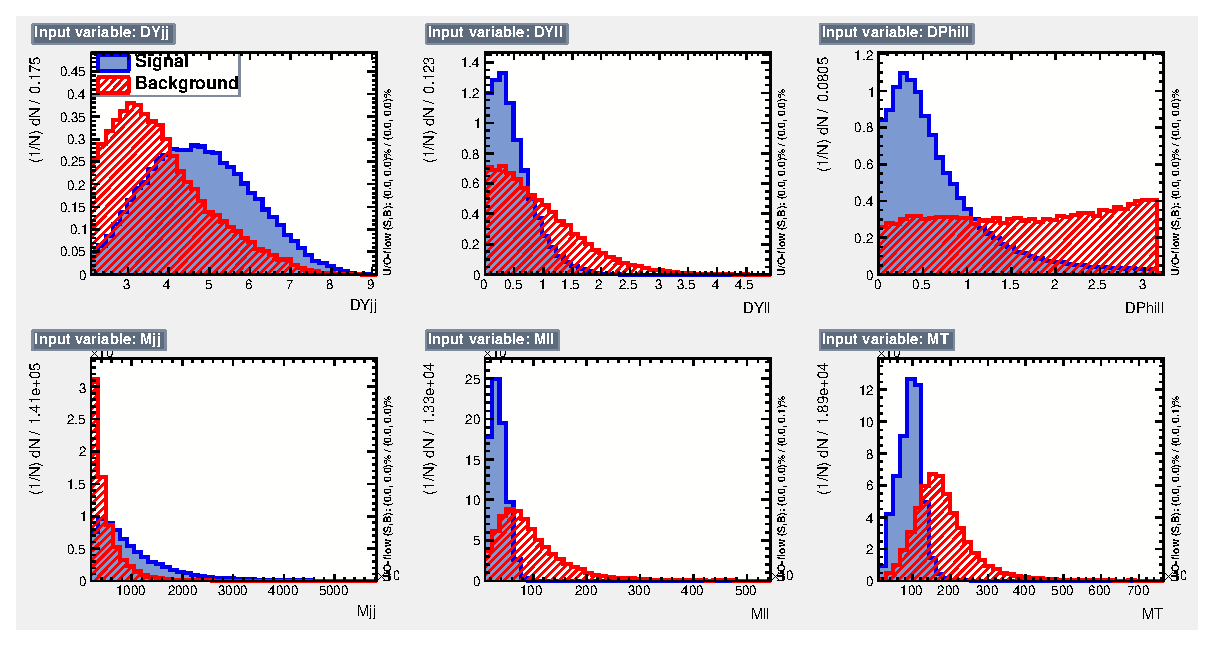
\includegraphics[width=0.45\linewidth]{Pictures/VBFvsWW+Top/variables_id_c1.eps}
    \includegraphics[width=0.45\linewidth]{Pictures/VBFvsWW+Top/variables_id_c2.eps}
    \caption{Distributions of input variables to VBF vs. top+$WW$ BDT. Samples are weighted and normalized to even numbers of background and signal events. Signal represents VBF and background top+$WW$.}.
    \label{fig:SRBDTinput}
\end{figure}
\begin{figure}[!htbp]
\centering
  \includegraphics[width=.4\linewidth]{Pictures/VBFvsWW+Top/CorrelationMatrixS.eps}
  \includegraphics[width=.4\linewidth]{Pictures/VBFvsWW+Top/CorrelationMatrixB.eps}
\caption{Correlations of input variables to VBF vs. top +$WW$ BDT. Signal represents VBF and background top+$WW$.}
\label{fig:SRcorrSB}
\end{figure}
The BDT training successfully separates VBF signal and top/$WW$ background. These backgrounds are considered together both because they have very similar signatures compared to the VBF signal and because our overall fit uses one parameter to estimate both $WW$ and top backgrounds together. In order to quantify the discrimination we use the integrated-ROC calculated through TMVA for weighted normalized samples and find an optimal value of 0.960. Comparisons between the test and training show that the BDT is un-biased- differences between testing and training samples would imply overtraining, or the BDT using to many parameters on too few events. Visually, once can see that the testing and trainings samples are quite similar. Additionally, a Kolmogorov-Smirnov test is performed to measure if the two test and training distributions differ significantly. If the two distributions are random samples of the same parent distribution, the KS-test would give a uniformly distributed value between zero and one (or an average value of 0.5). The closer to 0.5 the KS-test, the greater likelihood the curves come from the same parent, however this calculation is heavily skewed toward lower values so any value above zero (or not very close to zero, on order $10^{-4}$) can be considered not indicative of overtraining. For signal and background we find KS-test values of 0.107 and 0.154, and so no evidence of over-training. We can visualize the BDT output variable both on un-weighted normalized samples and on samples with all event weights applied. The following plot shows BDT results applied to normalized samples of VBF signal and top/$WW$ backgrounds.

\begin{figure}[!htbp]
\centering
  \includegraphics[width=.45\linewidth]{Pictures/VBFvsWW+Top/overtrain_BDTG.eps}
  \includegraphics[width=.35\linewidth]{Pictures/run2-emme-CutVBF_ZttBDT-BDT_VBF-log.pdf}
\caption{Unweighted, normalized samples of VBF (signal) and top$+WW$ samples (background) plotted over BDT output distribution on left, overlaid testing and training samples shown. Right, full weighted samples of VBF signal and all backgrounds plotted over BDT output distribution after signal region selection. Data is blinded here}
\label{fig:SRBDTresult}
\end{figure}

We aim to fit this distribution in the signal region with high significance in uppermost bins of the distribution. Since this BDT is trained and applied in the signal region we cannot directly test the modelling of input variables. However, modelling at the pre-selection level for each of these variables, shown earlier in the chapter show no evidence of mis-modelling. The binning for this discriminant used in the statistical fit and its result (using Asimov data) are shown in the final chapter. 

\clearpage
%-------------------------------------------------------------------------------
%-------------------------------------------------------------------------------
%-------------------------------------------------------------------------------
\chapter{Backgrounds and Systematics}
\label{sec:BackgroundsSys}
%{Backgrounds and systematics}
\section{Backgrounds}
While the VBF $H\rightarrow WW\rightarrow \ell\nu\ell\nu$ channel gives a fairly clear signal with $E_{\text{T}}^{\text{miss}}$, two leptons, and 2 jets, there are substantial backgrounds with similar final states. These include Drell-Yan processes (in which a $Z$ boson is formed from quark anti-quark annihilation of the two colliding protons), top quark final states (predominantly $t\bar{t}$), diboson events (led by SM $WW$ events), Higgs decays from the other production modes (mainly ggF), and background from mis-identified leptons, called fakes. In this section I will detail each background and describe our methods for estimating their role in overall results. I will describe how this analysis estimates and minimizes contributions from each background process. Finally, I will measure the purity and validate the modelling of these backgrounds by using events in ``control'' and ``validation'' regions. These regions are designed to select for particular backgrounds to use in the final statistical fit, ``control regions'', orto test that backgrounds overall modelling, ``validation regions''.  I made key contributions in this analysis in optimizing and testing control region definitions and their effects on our overall results. 

\subsection{Drell-Yan background ($Z\rightarrow \tau\tau$)}
The Drell-Yan background is produced in the initial collision when two quarks produce a $Z$ boson which then decays to two leptons. In this analysis we select two different flavor leptons in order to reject large Drell-Yan backgrounds in which the $Z$ decays to two electrons or two muons. However, our signal is still contaminated by Drell-Yan decays where the $Z$ decays to two $\tau$ leptons. We select events where one $\tau$ decays to an electron and the other to a muon. There are two jets and two leptons in this the Drell-Yan final state as well as missing energy from neutrinos, all of which are indicative of signal VBF Higgs events. The Feynman diagram for a typical Drell-Yan event is shown in Figure \ref{fig:DrellYan}. 

\begin{figure}
\centering
  \includegraphics[width=.35\linewidth]{Pictures/FeynmanDrellYan.png}
\caption{Feynman diagram for Drell-Yan process in which two quarks produce a photon or $Z$-boson that then decays leptonically \cite{DrellYan}.}
\label{fig:DrellYan}
\end{figure}

Removing events in a 25 GeV window about the $Z$-mass peak drastically improves $Z+$jets purity from only 19$\%$ of total events to approximately $52\%$. 

We have also tested and trained a secondary discriminant for $Z+$jets in our analysis, a BDT trained to discriminate $Z+$jets and VBF signal events. This BDT significantly decreases overall $Z+$jets background in our signal region but we found that the subsequent decrease in statistics from using this cut leads to very similar overall results. The results from this comparison are shown in Appendix II. 

\subsubsection{Drell-Yan Control Region}

The $Z+$jets control region definition is quite similar to the VBF signal region except that the $Z+$jets veto cut is inverted. Thus instead of removing events near the $Z$-mass window we select for them by applying a cut on $m_{ll}<80$ GeV,  66.2 GeV $< m_{\tau\tau}< 116.2$ GeV, and the same OLV and CJV cuts as in the VBF signal region. The $Z+$jets control region has a purity of $\approx 82\%$ and yields in this region are shown in the table \ref{tab:zttcr}.

\begin{table}[h!]
\scalebox{0.55}{

\begin{tabular}{ r ||r  r  r | r | r  r  r | r   r }
\ensuremath{\mathcal{L}=139 fb^{-1}} & $H_{VBF}$ & $H_{ggF}$ & $H_{VH}/ttH$ & Diboson & Top & Zjets & Mis-Id & Data & Data/MC\tabularnewline
\hline
$\vert m_{\tau\tau}-m_Z\vert<$25& \ensuremath{27} & \ensuremath{84} & \ensuremath{102} & \ensuremath{2540} & \ensuremath{5635} & \ensuremath{8909} & \ensuremath{417}   & \ensuremath{16400} & \ensuremath{0.93\pm 0.01}\tabularnewline
$M_{ll}<80$ GeV & \ensuremath{26} & \ensuremath{82} & \ensuremath{84} & \ensuremath{1082} & \ensuremath{1704} & \ensuremath{8675} & \ensuremath{232}  & \ensuremath{10805} & \ensuremath{0.91\pm 0.01}\tabularnewline
CJV$<20$ GeV & \ensuremath{21} & \ensuremath{59} & \ensuremath{64} & \ensuremath{791} & \ensuremath{1151} & \ensuremath{6474} & \ensuremath{185} & \ensuremath{7931} & \ensuremath{0.91\pm 0.01}\tabularnewline
OLV & \ensuremath{16} & \ensuremath{14} & \ensuremath{21} & \ensuremath{157} & \ensuremath{292} & \ensuremath{1393} & \ensuremath{15}   & \ensuremath{1832} & \ensuremath{0.96\pm 0.03}\tabularnewline
\hline
\end{tabular}

}
\caption{Cutflow in the $Z+$jets control region.}
\label{tab:zttcr}
\end{table}

Data/MC shows decent agreement over various variable distributions as seen in the plots \ref{fig:DYCR3}. Some of these variables are also used in the BDT described in Appendix II. 

\begin{figure}[!h]
\centering
  \subfloat[$m_{\tau\tau}$]{
      \includegraphics[width=0.3\textwidth]{Pictures/run2-emme-CutVBFZtautauControl_2jetinclOLV-mtt-lin.pdf}
  }\hfill
  \subfloat[$p^T_{tot}$]{
      \includegraphics[width=0.3\textwidth]{Pictures/run2-emme-CutVBFZtautauControl_2jetinclOLV-PtTot-lin.pdf}
  }\hfill
  \subfloat[$m_T$]{
      \includegraphics[width=0.3\textwidth]{Pictures/run2-emme-CutVBFZtautauControl_2jetinclOLV-MT-lin.pdf}
  }\hfill
  \subfloat[$E_{\text{T}}^{\text{miss}}$]{
      \includegraphics[width=0.3\textwidth]{Pictures/run2-emme-CutVBFZtautauControl_2jetinclOLV-MET-lin.pdf}
  }\hfill
  \subfloat[$\ensuremath{E_{\text{T,rel}}^{\text{miss}}}$]{
      \includegraphics[width=0.3\textwidth]{Pictures/run2-emme-CutVBFZtautauControl_2jetinclOLV-METRel-lin.pdf}
  }\hfill
  \subfloat[$\ensuremath{E_{\text{T}}^{\text{miss, significance}}}$]{
      \includegraphics[width=0.3\textwidth]{Pictures/run2-emme-CutVBFZtautauControl_2jetinclOLV-METSig-lin.pdf}
  }\hfill
  \subfloat[$\ensuremath{E_{\text{T}}^{\text{miss, track}}}$]{
      \includegraphics[width=0.3\textwidth]{Pictures/run2-emme-CutVBFZtautauControl_2jetinclOLV-TrackMET-lin.pdf}
  }\hfill
  \subfloat[$\ensuremath{E_{\text{T,rel}}^{\text{miss, track}}}$]{
      \includegraphics[width=0.3\textwidth]{Pictures/run2-emme-CutVBFZtautauControl_2jetinclOLV-TrackMETRel-lin.pdf}
  }%\hfill
 % \subfloat[$\ensuremath{\Delta\phi_{\ell\ell,E_{\text{T}}^{\text{miss, track}}}}$]{
 %     \includegraphics[width=0.3\textwidth]{Pictures/run2-emme-CutVBFZtautauControl_2jetinclOLV-DPhillMETtrk-lin.pdf}
 % }%\hfill 
{\caption{Distributions of $m_{\tau\tau}$, $p^T_{tot}$, $m_T$, $\ensuremath{E_{\text{T}}^{\text{miss}}}$, $\ensuremath{E_{\text{T, rel}}^{\text{miss}}}$, $\ensuremath{E_{\text{T}}^{\text{miss, significance}}}$, $\ensuremath{E_{\text{T}}^{\text{miss, track}}}$, and $\ensuremath{E_{\text{T,rel}}^{\text{miss, track}}}$ in the $Z+$jets control region.
\label{fig:DYCR3}}}
\end{figure}

Normalization factors (NF) are derived in the $Z+$jets control region to correct for Data/MC mis-modelling. These factors are applied to the $Z+$jets sample in the signal region. The NF factor used in this analysis is $1.01 \pm 0.04$. 

\subsection{Top background}
The top background consists of two main components, $Wt$ and $t\bar{t}$ events, where the $W$ decays leptonically and the top quarks decay to jets (notably $b$-jets). The top background is dominated by $t\bar{t}$ and is the largest background in our signal region, composing about $60\%$ of the total background. Though top backgrounds are numerous, discrimination between top and signal Higgs events is possible through training a BDT on variables that have very different discributions between these two types of events like $m_{\ell\ell}$ and $\Delta Y_{jj}$. As demonstrated in Chapter 4, our BDT discriminates between signal and top background quite well. The top background is therefore defined in the signal region and separated using the VBF vs. top$+WW$ discriminant. The final statistical fit seven total BDT discriminant and three of these are assocated with the top background: VBF vs. top$+WW$, top$+WW$ vs. all other samples, and top vs. $WW$. The overall statistical fit strategy is discussed in the following chapter but in this section I will describe the BDT used as the top discriminant: top$+WW$ vs. all other samples. 

We define a top validation region to test top Monte Carlo modelling and calculate a normalization factor used to correct top mis-modelling in the signal region. The top validation region is described similarly to the signal region with one major difference: the $b$- tagging selection applied in the signal region is (almost) reversed. Instead, we require exactly one $b$-tagged jet. The result is a highly pure top validation region, approximately $97\%$, where the flavor composition of the tagged jets is close to the signal region. Yields in this region are shown in the table \ref{tab:topcr}.

\begin{table}[h!]
\scalebox{0.55}{
%%% created on Thu Jun 11 11:37:17 2020 from TQSampleFolder 'samples' with TQLibrary UNKNOWN compiled with GCC 8.3.0 against ROOT 6.16/00
\providecommand{\xmark}{{\sffamily \bfseries X}}
\providecommand\rotatecell[2]{\rotatebox[origin=c]{#1}{#2}}
\begin{tabular}{ r ||r  r  r | r | r  r  r | r   r }
\ensuremath{\mathcal{L}=139 fb^{-1}} & $H_{VBF}$ & $H_{ggF}$ & $H_{VH}/ttH$ & Diboson & Top & Zjets & Mis-Id & Data & Data/MC\tabularnewline
\hline
$n_{b-jets} = 1$ & \ensuremath{39.79\pm 0.19} & \ensuremath{162.38\pm 1.34} & \ensuremath{89.41\pm 0.57} & \ensuremath{3922.22\pm 31.68} & \ensuremath{349820.12\pm 128.80} & \ensuremath{3683.96\pm 34.18} & \ensuremath{4601.97\pm 97.54} & \ensuremath{359758} & \ensuremath{0.99\pm 0.00}\tabularnewline
$Z\to\tau\tau$ veto & \ensuremath{18.05\pm 0.13} & \ensuremath{22.85\pm 0.50} & \ensuremath{5.66\pm 0.13} & \ensuremath{245.35\pm 12.82} & \ensuremath{30023.80\pm 38.13} & \ensuremath{180.86\pm 8.66} & \ensuremath{280.21\pm 28.51}  & \ensuremath{30709} & \ensuremath{1.00\pm 0.01}\tabularnewline
CJV $<20$ GeV & \ensuremath{29.69\pm 0.17} & \ensuremath{106.25\pm 1.08} & \ensuremath{62.42\pm 0.47} & \ensuremath{2518.28\pm 26.99} & \ensuremath{238659.28\pm 107.33} & \ensuremath{2487.15\pm 30.44} & \ensuremath{2941.00\pm 80.13} & \ensuremath{244811} & \ensuremath{0.99\pm 0.00}\tabularnewline
OLV & \ensuremath{20.85\pm 0.14} & \ensuremath{25.71\pm 0.53} & \ensuremath{13.85\pm 0.20} & \ensuremath{411.01\pm 13.96} & \ensuremath{46267.04\pm 47.47} & \ensuremath{499.81\pm 12.91} & \ensuremath{415.70\pm 35.23}\  & \ensuremath{47182} & \ensuremath{0.99\pm 0.00}\tabularnewline
$Z\to\tau\tau$ veto & \ensuremath{18.05\pm 0.13} & \ensuremath{22.85\pm 0.50} & \ensuremath{5.66\pm 0.13} & \ensuremath{245.35\pm 12.82} & \ensuremath{30023.80\pm 38.13} & \ensuremath{180.86\pm 8.66} & \ensuremath{280.21\pm 28.51} & \ensuremath{30709} & \ensuremath{1.00\pm 0.01}\tabularnewline
\hline
\end{tabular}

}
\caption{Cutflow in the top control region.}
\label{tab:topcr}
\end{table}

Data/MC in the top validation region shows good agreement over various variable distributions as seen in the  below. Many of these distributions are used as inputs to the top$+WW$ vs. all BDT. 

\begin{figure}[!h]
\centering
  \subfloat[$m_{\ell\ell}$]{
      \includegraphics[width=0.3\textwidth]{Pictures/run2-emme-CutVBFTopControl_2jetinclZttVeto-Mll-lin.pdf}
  }\hfill
  \subfloat[$\Delta Y_{\ell\ell}$]{
      \includegraphics[width=0.3\textwidth]{Pictures/run2-emme-CutVBFTopControl_2jetinclZttVeto-DYll-lin.pdf}
  }\hfill 
  \subfloat[$\Delta Y_{jj}$]{
      \includegraphics[width=0.3\textwidth]{Pictures/run2-emme-CutVBFTopControl_2jetinclZttVeto-DYjj-lin.pdf}
  }\hfill
  \subfloat[$\sum$ centralities]{
      \includegraphics[width=0.3\textwidth]{Pictures/run2-emme-CutVBFTopControl_2jetinclZttVeto-sumOfCentralitiesL-lin.pdf}
  }\hfill
%  \subfloat[$m_{jj}$]{
%      \includegraphics[width=0.3\textwidth]{Pictures/run2-emme-CutVBFTopControl_2jetinclZttVeto-Mjj-lin.pdf}
%  }\hfill
  \subfloat[$M_{l0j0}$]{
      \includegraphics[width=0.3\textwidth]{Pictures/run2-emme-CutVBFTopControl_2jetinclZttVeto-Ml0j0-lin.pdf}
  }\hfill
  \subfloat[$M_{l1j1}$]{
      \includegraphics[width=0.3\textwidth]{Pictures/run2-emme-CutVBFTopControl_2jetinclZttVeto-Ml1j1-lin.pdf}
  }\hfill
  \subfloat[$\Delta\Phi_{jj}$]{
      \includegraphics[width=0.3\textwidth]{Pictures/run2-emme-CutVBFTopControl_2jetinclZttVeto-DPhijj-lin.pdf}
  }\hfill
  \subfloat[$p_T^{tot}$]{
      \includegraphics[width=0.3\textwidth]{Pictures/run2-emme-CutVBFTopControl_2jetinclZttVeto-PtTot-lin.pdf}
  }\hfill
  \subfloat[$m_T$]{
      \includegraphics[width=0.3\textwidth]{Pictures/run2-emme-CutVBFTopControl_2jetinclZttVeto-MT-lin.pdf}
  }%hfill
% \subfloat[$\ensuremath{E_{\text{T}}^{\text{miss}}}$]{
%     \includegraphics[width=0.3\textwidth]{Pictures/run2-emme-CutVBFTopControl_2jetinclZttVeto-MET-lin.pdf}
% }%\hfill 
{\caption{Distributions of $m_{\ell\ell}$, $\Delta Y_{\ell\ell}$, $\Delta Y_{jj}$, $\sum$ centralities, $M_{l0j0}$, $M_{l1j1}$, $\Delta\Phi_{jj}$, $p_T^{tot}$, and $m_T$ in the top validation region.
\label{fig:TopCR3}}}
\end{figure}

\subsubsection{Top$+WW$ BDT discriminant}

The top$+WW$ BDT is trained after the VBF selection and applied in the same phase space. The training includes top and $WW$ trained against weighted samples of VBF, ggF, $Z+$jets, and $V\gamma$ events. There are about 90,000 un-weighted $WW$ and top events corresponding to approximately 2000 weighted events and about 115,000 un-weighted VBF, ggF, $Z+$jets and $V\gamma$ events corresponding to 550 weighted events. The same BDT training interface and strategy discussed in Chapter 5 is used again here. The final set of testing parameters is summarized in Table~\ref{tab:TopBDTparameters}.

\begin{table}[h!]
\centering
\begin{tabular}{|l|c|}
\hline
Parameter                                    & Value     \\
\hline
Boosting algorithm                           &  Gradient  \\
Maximum tree depth                           &  22       \\
Number of trees                              &  200     \\
Minimum number of events requires per mode   &  5\%      \\
Number of cuts                               &  7        \\
\hline
\end{tabular}
\caption{BDT parameters used for the top + $WW$ vs. other backgrounds training.} 
\label{tab:TopBDTparameters}
\end{table}

This BDT utilizes 8 lepton and jet kinematic variables to distinguish between top$+WW$ and other events. These include $\Delta Y_{jj}$, the combination of lepton/jet masses $M_{l0j0}$ for leading and subleading leptons and jets, $\Delta \Phi_{\ell\ell}$, $m_T$, $\eta_{j0}$, $\eta_{j1}$, $\Delta \Phi_{jj}$, and $\sum$ centralities (L). Plots shown in \ref{fig:TopBDTinput} and \ref{fig:TopcorrSB} demonstrate the input distributions used to train the BDT and their correlations.

\begin{figure}[!htbp]
    \centering
    \includegraphics[width=0.55\linewidth]{Pictures/Top+WWvsEverything/variables_id_c1.eps}
    \includegraphics[width=0.55\linewidth]{Pictures/Top+WWvsEverything/variables_id_c2.eps}
    \caption{Distributions of input variables to top+$WW$ vs. other samples BDT. Samples are weighted and normalized to even numbers of background and signal events. Signal represents top+$WW$ and background all other samples (S. Addepalli).}.
    \label{fig:TopBDTinput}
\end{figure}
\begin{figure}[!htbp]
\centering
  \includegraphics[width=.3\linewidth]{Pictures/Top+WWvsEverything/CorrelationMatrixS.eps}
  \includegraphics[width=.3\linewidth]{Pictures/Top+WWvsEverything/CorrelationMatrixB.eps}
\caption{Correlations of input variables to top +$WW$ vs other samples BDT. Signal represents top+$WW$ and background other samples (S. Addepalli).}
\label{fig:TopcorrSB}
\end{figure}
The BDT training successfully separates top/$WW$ background and other samples (ggF, VBF, $Z+$jets, and $V\gamma$). We calculate an integrated-ROC value of 0.920. For signal and background we find KS-test values of 0.107 and 0.154 respectively, and so no evidence of over-training. The BDT output variables are shown both on weighted normalized samples and on samples with full event weights applied in \ref{fig:TopBDTresult}.

\begin{figure}[!htbp]
\centering
  \includegraphics[width=.4\linewidth]{Pictures/Top+WWvsEverything/overtrain_BDTG.eps}
  \includegraphics[width=.45\linewidth]{Pictures/run2-emme-CutVBFDYjjMin-BDT_TopWWAll-lin.pdf}
\caption{Weighted, normalized samples of top$+WW$ samples (signal) and other samples (background) plotted over BDT output distribution on left, overlaid testing and training samples shown. Right, full weighted samples of all signal and background events plotted over BDT output distribution after signal region selection (S. Addepalli).}
\label{fig:TopBDTresult}
\end{figure}

We aim to fit this distribution in the signal region with high significance for top/$WW$ events in the uppermost bins of the distribution. Since this BDT is trained and applied in the signal region, we cannot directly test the modelling of input variables. However, modelling at the pre-selection level for each of these variables as well as in the top validation region described eariler show no evidence of mis-modelling. The binning for this discriminant used in the statistical fit and its result are shown in Chapter 7.

%\begin{figure}[!htbp]
%\centering
%\includegraphics[width=.5\linewidth]{Pictures/run2-emme-CutVBFTopControl_2jetinclZttVeto-BDT_TopWWAll-lin.pdf}
%\caption{Full weighted samples of all signal and background plotted over Top + $WW$ vs. VBF ggF + $Z+$jets +$V\gamma$ BDT output distributions in top validation region}
%\label{fig:VBFTopWWBDTVR}
%\end{figure}
%
%The BDT to discriminate top$+WW$ background from VBF signal events is trained and applied in the signal region and so described in the previous chapter, but its distribution in the top validation region is also shown. 
%
%\begin{figure}[!htbp]
%\centering
%\includegraphics[width=.5\linewidth]{Pictures/run2-emme-CutVBFTopControl_2jetinclZttVeto-BDT_VBF-lin.pdf}
%\caption{Full weighted samples of all signal and background plotted over Top + $WW$ vs. VBF BDT output distributions in top validation region}
%\label{fig:VBFTopWWBDTVR}
%\end{figure}
%
%A designated BDT discriminates between top and WW backgrounds and is described further in the WW background section (next). However, this distribution in the top validation region with all weighted samples is shown below. to demonstrate its effect on primarily predominantly top-like events.

%\begin{figure}[!htbp]
%\centering
%\includegraphics[width=.5\linewidth]{Pictures/run2-emme-CutVBFTopControl_2jetinclZttVeto-BDT_TopWW-lin.pdf}
%\caption{Full weighted samples of all signal and background plotted over Top vs. $WW$ BDT output distributions in top validation region}
%\label{fig:TopWWBDTVR}
%\end{figure}

Normalization factors (NF) are derived in the top validation region to correct for data/MC mis-modelling. These factors are applied to the top sample in the signal region. The NF factor used in this analysis is $0.99\pm0.01$. 

\subsection{Diboson background}

The $WW$ background consists primarily of QCD $WW$+jets events (highly dominating electroweak vertices). This background is estimated along with the top background using a joint parameter due to their similarities in signature as well as the difficulty in defining a pure $WW$ control region without top contamination. A $WW$ validation region is defined to demonstrate $WW$ MC modelling in a targeted $WW$ region.  The $WW$ validation region is defined by requiring at least 2 jets, a $b$-veto ($N_{b-jet}<1$) and a central-jet-veto of below $20$ GeV as in the signal region. Two additional cuts differ from the signal region: $m_T>130$ GeV and $m_{T2}>160$ GeV. $m_{T2}$, or the stransverse mass, is used to describe a lower bound on a pair-production parent particle's mass. $m_{T2}$ is calculated as the minimum $m_T(m_{\text{inv}},\vec{p_T^i})$ for all values of $p_T^1$ and $p_T^2$ which satisfy $\vec{p_T^1}+\vec{p_T^2}=\vec{p_T^{\text{miss}}}$ \cite{MT2}. This can be summarized as
\begin{equation}
m_{T2}=\text{min}_{\vec{p_T^1},\vec{p_T^2}}(\text{max}(m_T(m_{\text{inv}},\vec{p_T^1}),m_T(m_{\text{inv}},\vec{p_T^2}))).
\end{equation}
where $m_{\text{inv}}$ is zero in this analysis. Requiring $m_{T2}>160$ GeV eliminates contamination from many $t\bar{t}$ decays which have an upper limit near the top mass. The purity of the $WW$ validation region is $\approx 37\%$ and the cutflow for this region is shown \ref{tab:wwvr}.

\begin{table}[h!]
\scalebox{0.55}{
%%% created on Thu Jun 11 11:37:17 2020 from TQSampleFolder 'samples' with TQLibrary UNKNOWN compiled with GCC 8.3.0 against ROOT 6.16/00
\providecommand{\xmark}{{\sffamily \bfseries X}}
\providecommand\rotatecell[2]{\rotatebox[origin=c]{#1}{#2}}
\begin{tabular}{ r ||r  r  r | r | r  r  r | r   r }
\ensuremath{\mathcal{L}=139 fb^{-1}} & $H_{VBF}$ & $H_{ggF}$ & $H_{VH}/ttH$ & Diboson & Top & Zjets & Mis-Id & Data & Data/MC\tabularnewline
\hline
b-veto & \ensuremath{324} & \ensuremath{1110} & \ensuremath{438} & \ensuremath{25107} & \ensuremath{63788} & \ensuremath{22151} & \ensuremath{3794} & \ensuremath{109677} & \ensuremath{0.94\pm 0.00}\tabularnewline
$M_{T}>$130 GeV & \ensuremath{32} & \ensuremath{155} & \ensuremath{60} & \ensuremath{18021} & \ensuremath{50088} & \ensuremath{872} & \ensuremath{1784}  & \ensuremath{68255} & \ensuremath{0.96\pm 0.00}\tabularnewline
$M_{T2}>$160 GeV & \ensuremath{19} & \ensuremath{62} & \ensuremath{17} & \ensuremath{7272} & \ensuremath{11553} & \ensuremath{302} & \ensuremath{516} & \ensuremath{18672} & \ensuremath{0.95\pm 0.01}\tabularnewline
CJV (20GeV) & \ensuremath{14} & \ensuremath{41} & \ensuremath{11} & \ensuremath{4861} & \ensuremath{6416} & \ensuremath{185} & \ensuremath{328}  & \ensuremath{11245} & \ensuremath{0.95\pm 0.01}\tabularnewline
\hline
\end{tabular}

}
\caption{Cutflow in the $WW$ validation region.}
\label{tab:wwvr}
\end{table}

Data/MC shows good agreement over various variable distributions as shown in \ref{fig:WWCR3}.
\begin{figure}[!h]
\centering
%  \subfloat[$m_{\ell\ell}$]{
%      \includegraphics[width=0.3\textwidth]{Pictures/run2-emme-CutVBFWWControl_CJV20-Mll-lin.pdf}
%  }\hfill
  \subfloat[$\Delta Y_{\ell\ell}$]{
      \includegraphics[width=0.3\textwidth]{Pictures/run2-emme-CutVBFWWControl_CJV20-DYll-lin.pdf}
  }\hfill
  \subfloat[$\Delta Y_{jj}$]{
      \includegraphics[width=0.3\textwidth]{Pictures/run2-emme-CutVBFWWControl_CJV20-DYjj-lin.pdf}
  }\hfill
  \subfloat[$\sum$ centralities]{
      \includegraphics[width=0.3\textwidth]{Pictures/run2-emme-CutVBFWWControl_CJV20-sumOfCentralitiesL-lin.pdf}
  }\hfill
  \subfloat[$M_{l0j0}$]{
      \includegraphics[width=0.3\textwidth]{Pictures/run2-emme-CutVBFWWControl_CJV20-Ml0j0-lin.pdf}
  }\hfill
  \subfloat[$M_{l1j1}$]{
      \includegraphics[width=0.3\textwidth]{Pictures/run2-emme-CutVBFWWControl_CJV20-Ml1j1-lin.pdf}
  }\hfill
  \subfloat[$p_T^{j0}$]{
      \includegraphics[width=0.3\textwidth]{Pictures/run2-emme-CutVBFWWControl_CJV20-leadJetPt-lin.pdf}
  }\hfill
%  \subfloat[$m_{jj}$]{
%      \includegraphics[width=0.3\textwidth]{Pictures/run2-emme-CutVBFWWControl_CJV20-Mjj-lin.pdf}
%  }\hfill
  \subfloat[$\Delta\Phi_{jj}$]{
      \includegraphics[width=0.3\textwidth]{Pictures/run2-emme-CutVBFWWControl_CJV20-DPhijj-lin.pdf}
  }\hfill
  \subfloat[$p^T_{tot}$]{
      \includegraphics[width=0.3\textwidth]{Pictures/run2-emme-CutVBFWWControl_CJV20-PtTot-lin.pdf}
  }\hfill
  \subfloat[$m_T$]{
      \includegraphics[width=0.3\textwidth]{Pictures/run2-emme-CutVBFWWControl_CJV20-MT-lin.pdf}
  }%\hfill
%  \subfloat[$\ensuremath{E_{\text{T,rel}}^{\text{miss}}}$]{
%      \includegraphics[width=0.3\textwidth]{Pictures/run2-emme-CutVBFWWControl_CJV20-MET-lin.pdf}
%  }%\hfill 
{\caption{Distributions of $\Delta Y_{\ell\ell}$, $\Delta Y_{jj}$, $\sum$ centralities, $M_{l0j0}$, $M_{l1j1}$, $p_T^{j0}$, $\Delta\Phi_{jj}$, $p^T_{tot}$, and $m_T$ in the $WW$ validation region.
\label{fig:WWCR3}}}
\end{figure}

\subsubsection{Top vs. $WW$ BDT discriminant}

Another BDT discriminant is trained in the signal region to differentiate between $top$ and $WW$ background events. Both the $top$ and $WW$ backgrounds are estimated with one parameter within the signal region. Within the signal region phase space we split the top and $WW$ events into control regions based on the top vs. $WW$ BDT discriminant. This training is not as successful at classification as the BDTs discussed previously, but its use in the final statistical fit is still beneficial. The training includes weighted samples of top and $WW$ events trained against one another. The training uses about 35,000 un-weighted and 1500 weighted top events and approximately 55,000 un-weighted and 500 weighted $WW$ events. Optimal parameters for the training are summarized in Table~\ref{tab:WWBDTparameters}.
\begin{table}[h!]
\centering
\begin{tabular}{|l|c|}
\hline
Parameter                                    & Value     \\
\hline
Boosting algorithm                           &  Gradient  \\
Maximum tree depth                           &  22       \\
Number of trees                              &  200     \\
Minimum number of events requires per mode   &  5\%      \\
Number of cuts                               &  7        \\
\hline
\end{tabular}
\caption{Parameters used for the top vs. $WW$ BDT training.} 
\label{tab:WWBDTparameters}
\end{table}

This BDT employs 14 kinematic variables to distinguish between top and $WW$ events. These include $\Delta Y_{jj}$, $\Delta Y_{\ell\ell}$, $\Delta \Phi_{\ell\ell}$, $m_T$, $\eta_{l0}$, $\eta_{l1}$, $p^T_{j0}$, $p^T_{j1}$, $\Delta \Phi_{jj}$, $\sum$ centralities (L), and combined masses $M_{l0j0}$, $M_{l0j1}$, $M_{l1j0}$, $M_{l1j1}$. Plots shown in \ref{fig:WWBDTinput} and \ref{fig:WWcorrSB} demonstrate the input distributions used to train the BDT and their correlations.
\begin{figure}[!htbp]
    \centering
    \includegraphics[width=0.55\linewidth]{Pictures/TopvsWW/variables_id_c1.eps}
    \includegraphics[width=0.55\linewidth]{Pictures/TopvsWW/variables_id_c2.eps}
    \caption{Distributions of input variables to top vs. $WW$ BDT. Samples are weighted and normalized to even numbers of background and signal events. Signal represents top and background $WW$ (S. Addepalli).}.
    \label{fig:WWBDTinput}
\end{figure}
\begin{figure}[!htbp]
\centering
  \includegraphics[width=.3\linewidth]{Pictures/TopvsWW/CorrelationMatrixS.eps}
  \includegraphics[width=.3\linewidth]{Pictures/TopvsWW/CorrelationMatrixB.eps}
\caption{Correlations of input variables to top vs. $WW$ BDT. Signal represents top and background $WW$ (S. Addepalli).}
\label{fig:WWcorrSB}
\end{figure}

Despite the BDT training, it is difficult to separate top and $WW$ backgrounds because the signals have similar kinematic distributions that make high discrimination difficult. The integrated-ROC calculated for weighted normalized samples is 0.653. While relatively low, this shows some minimal amount of discrimination. This is useful in the fit to differentiate top and $WW$ backgrounds, though high levels of separation are not necessary because top and $WW$ are estimated together with a shared parameter in the simultaneous fit. For signal and background we find KS-test values of 0.067 and 0.037 showing no evidence of over-training. The BDT output variable is visualized on weighted normalized samples and on samples with all event weights applied in \ref{fig:WWBDTresult}. 

\begin{figure}[!htbp]
\centering
  \includegraphics[width=.45\linewidth]{Pictures/TopvsWW/overtrain_BDTG.eps}
  \includegraphics[width=.35\linewidth]{Pictures/run2-emme-CutVBFDYjjMin-BDT_TopWW-lin.pdf}
\caption{Weighted, normalized samples of top samples (signal) and $WW$ samples (background) plotted over BDT output distribution on left, overlaid testing and training samples shown. Right, full weighted samples of all signal and background events plotted over the BDT output distribution after signal region selection (S. Addepalli).}
\label{fig:WWBDTresult}
\end{figure}

\subsection{ggF background}
Other Higgs production modes are considered backgrounds in this analysis. Vector mediated Higgs production ($VH$) and top produced Higgs ($ttH$) are small in our signal region so do not play a large role in the analysis. ggF Higgs production, however, does represent a significant background. Signal region cuts requiring at least 2-jets and the central jet veto significantly reduce background yields, but because ggF is kinematically very similar to VBF signal, it still has a large effect on the VBF coupling measurement. To mitigate these effects, ggF events are simultaneously estimated from three control regions and the signal region. The control regions are chosen to minimize both the statistical and the modelling uncertainties, in particular those originating from the modelling of higher order QCD corrections. The regions begin with a subdivision based on the jet multiplicity. The first two regions, ggF CR1 and ggF CR2, are built from all preselection cuts and cuts requiring at least two jets, a $b$-veto, $Z\rightarrow\tau\tau$-veto, and orthogonal cuts on the central jet veto (CJV) and opposite lepton veto (OLV). The third ggF control region, ggF CR3, uses all preselection cuts, a $b$ veto, $Z\rightarrow \tau\tau$ veto, and requirement for less than 2 jets. The full definitions are described:  
\begin{itemize} 
\item {\textbf GGF-CR1:} Preselection criteria and $N_{ \text{jet}}>=2$, $b$ veto, $Z\rightarrow\tau\tau$ veto, $\text{CJV} > 1$ and $\text{OLV} > 1$. 
\item {\textbf GGF-CR2:} Preselection criteria and $N_{ \text{jet}}>=2$, $b$ veto, $Z\rightarrow\tau\tau$ veto, $\text{CJV}<1$ and $\text{OLV}>1$ or $\text{CJV}>1$ and $\text{OLV}<1$.
\item {\textbf GGF-CR3:} Preselection criteria and $N_{ \text{jet}}>=2$, $b$ veto, and $Z\rightarrow\tau\tau$ veto. 
\end{itemize} 
The full ggF expectation in the signal region is built from the following ratio (inspired by the ABCD method \cite{ABCD}) 
\begin{equation}
	\mu_{{\text GGF-SR}} = \frac{\mu^{{\text GGF-CR}}_{1} \cdot\mu^{{\text GGF-CR}}_{3}}{ \mu^{{\text GGF-CR}}_{2}}.
\end{equation}
where $\mu_{\text{ggF}}$ represents the yield modifier in each ggF control region. In each ggF category the ggF yield is extracted from simulation-extracted template fits based on dedicated discriminants. For each control region a dedicated multivariate discriminant is trained and applied to discriminate between ggF and all other samples. Results and training parameters from each of these discriminants is summarized next.

\subsubsection{Discriminant in ggF CR1}
The multivariate discriminant used for ggF CR1 is a boosted decision tree (BDT) trained after the ggF CR1 selection. The training includes ggF events trained against VBF signal and all backgrounds with about 8,000 ggF events (70 weighted) and 250,000 other events (5,000 weighted). The optimal parameters for training are summarized in Table~\ref{tab:ggFCR1BDTparameters}.
\begin{table}[h!]
\centering
\begin{tabular}{|l|c|c|}
\hline
Parameter                                    & Value     \\
\hline
Boosting algorithm                           & Gradient \\
Maximum tree depth                           &  10      \\
Number of trees                              &  600    \\
Minimum number of events requires per mode   &  5\%     \\ 
Number of cuts                               &  7       \\
\hline
\end{tabular}
\caption{BDT parameters used for the ggF CR1 training.}
\label{tab:ggFCR1BDTparameters}
\end{table}
 
For this BDT 8 kinematic distributions are used to take advantage of differences in distributions between ggF events and other sample types. These variables include $\Delta Y_{\ell\ell}$, $\Delta \Phi_{\ell\ell}$,$m_{\ell\ell}$,$m_T$, jet $p^T_{\text{lead}}$, jet $p^T_{\text{sublead}}$, $\Delta \Phi_{jj}$, and $\ensuremath{E_{\text{T}}^{\text{miss}}}$. Distributions for these variables in the ggF CR1 region where the BDT is trained are shown in \ref{fig:ggFCR1} demonstrating data/MC modelling for each.

\begin{figure}[!h]
  \subfloat[$\Delta Y_{\ell\ell}$]{
      \includegraphics[width=0.3\textwidth]{Pictures/run2-emme-CutVBFggFCR1-DYll-lin.pdf}
  }\hfill
  \subfloat[$\Delta \Phi_{\ell\ell}$]{
      \includegraphics[width=0.3\textwidth]{Pictures/run2-emme-CutVBFggFCR1-DPhill-lin.pdf}
  }\hfill
  \subfloat[$m_{\ell\ell}$]{
      \includegraphics[width=0.3\textwidth]{Pictures/run2-emme-CutVBFggFCR1-Mll-lin.pdf}
  }\hfill
  \subfloat[$m_T$]{
      \includegraphics[width=0.3\textwidth]{Pictures/run2-emme-CutVBFggFCR1-MT-lin.pdf}
  }\hfill
  \subfloat[jet $p^T_{\text{lead}}$]{
      \includegraphics[width=0.3\textwidth]{Pictures/run2-emme-CutVBFggFCR1-leadJetPt-lin.pdf}
  }\hfill
  \subfloat[jet $p^T_{\text{sublead}}$]{
      \includegraphics[width=0.3\textwidth]{Pictures/run2-emme-CutVBFggFCR1-subleadJetPt-lin.pdf}
  }\hfill
  \subfloat[$\Delta \Phi_{jj}$]{
      \includegraphics[width=0.3\textwidth]{Pictures/run2-emme-CutVBFggFCR1-DPhijj-lin.pdf}
  }\hfill
  \subfloat[$\ensuremath{E_{\text{T}}^{\text{miss}}}$]{
      \includegraphics[width=0.3\textwidth]{Pictures/run2-emme-CutVBFggFCR1-MET-lin.pdf}
  }%\hfill
{\caption{Distributions of $\Delta Y_{\ell\ell}$, $\Delta \Phi_{\ell\ell}$,$m_{\ell\ell}$,$m_T$, jet $p^T_{\text{lead}}$, jet $p^T_{\text{sublead}}$, $\Delta \Phi_{jj}$, and $\ensuremath{E_{\text{T}}^{\text{miss}}}$ in the ggF CR1 used as input to the BDT discriminating ggF from all other samples.
\label{fig:ggFCR1}}}
\end{figure} 

Plots shown in \ref{fig:ggFCR1BDTinput} and \ref{fig:ggFCR1corrSB} demonstrate the input distributions used to train the BDT and their correlations where each distribution is normalized to equal number of background and signal events. 

\begin{figure}[!htbp]
    \centering
    \includegraphics[width=0.55\linewidth]{Pictures/ggFCR1/variables_id_c1.eps}
    \includegraphics[width=0.55\linewidth]{Pictures/ggFCR1/variables_id_c2.eps}
    \caption{Distributions of input variables to ggF CR1 BDT. Samples are weighted and normalized to even numbers of background and signal events. Signal represents ggF and background all other samples (S. Addepalli).}.
    \label{fig:ggFCR1BDTinput}
\end{figure}
\begin{figure}[!htbp]
\centering
  \includegraphics[width=.3\linewidth]{Pictures/ggFCR1/CorrelationMatrixS.eps}
  \includegraphics[width=.3\linewidth]{Pictures/ggFCR1/CorrelationMatrixB.eps}
\caption{Correlations of input variables to ggF CR1 BDT. Signal represents ggF and background all other samples (S. Addepalli).}
\label{fig:ggFCR1corrSB}
\end{figure}

The BDT has an integrated-ROC value of 0.898, demonstrating successful classification. Comparisons between the test and training show that the BDT is un-biased and a KS-test (values 0.191, 0.049 for signal, background) demonstrates this. The BDT output variable is visualized on weighted normalized samples and on samples without normalization in \ref{fig:ggFCR1BDTresult}.

\begin{figure}[!htbp]
\centering
  \includegraphics[width=.4\linewidth]{Pictures/ggFCR1/overtrain_BDTG.eps}
  \includegraphics[width=.45\linewidth]{Pictures/run2-emme-CutVBFggFCR1-BDT_ggFCR1-log.pdf}
\caption{Normalized samples of ggF (signal) and all other samples (background) plotted over BDT output distribution on left, overlaid testing and training samples shown. Right, full weighted samples of ggF signal and all other backgrounds plotted over BDT output distribution after ggF CR 1 (S. Addepalli).}
\label{fig:ggFCR1BDTresult}
\end{figure}

\subsubsection{Discriminant in ggF CR2}

The ggF CR2 BDT discriminant is trained using all ggF CR2 selection criteria. The training includes about 2,000 unweighted (300 weighted) ggF events trained against 90,000 un-weighted (1500 weighted) other samples. The optimal training parameters are summarized in Table~\ref{tab:ggFCR2BDTparameters}.
\begin{table}[h!]
\centering
\begin{tabular}{|l|c|c|}
\hline
Parameter                                    & Value     \\
\hline
Boosting algorithm                           & Gradient \\
Maximum tree depth                           &  10      \\
Number of trees                              &  50    \\
Minimum number of events requires per mode   &  5\%     \\ 
Number of cuts                               &  7       \\
\hline
\end{tabular}
\caption{BDT parameters used for the ggF CR2 training.}
\label{tab:ggFCR2BDTparameters}
\end{table}

Six lepton and jet kinematic distributions are used, including $\Delta Y_{\ell\ell}$, $\Delta \Phi_{\ell\ell}$,$m_{\ell\ell}$,$m_T$, $\Delta \Phi_{jj}$, and $\ensuremath{E_{\text{T}}^{\text{miss}}}$. Distributions for these variables in the ggF CR2 region are shown in \ref{fig:ggFCR2} and demonstrate data/MC modelling.
\begin{figure}[!h]
  \subfloat[$\Delta Y_{\ell\ell}$]{
      \includegraphics[width=0.3\textwidth]{Pictures/run2-emme-CutVBFggFCR2-DYll-lin.pdf}
  }\hfill
  \subfloat[$\Delta \Phi_{\ell\ell}$]{
      \includegraphics[width=0.3\textwidth]{Pictures/run2-emme-CutVBFggFCR2-DPhill-lin.pdf}
  }\hfill
  \subfloat[$m_{\ell\ell}$]{
      \includegraphics[width=0.3\textwidth]{Pictures/run2-emme-CutVBFggFCR2-Mll-lin.pdf}
  }\hfill
  \subfloat[$m_T$]{
      \includegraphics[width=0.3\textwidth]{Pictures/run2-emme-CutVBFggFCR2-MT-lin.pdf}
  }\hfill
%  \subfloat[$p^T_{tot}$]{
%      \includegraphics[width=0.3\textwidth]{Pictures/run2-emme-CutVBFggFCR2-PtTot-lin.pdf}
%  }\hfill
%  \subfloat[lep $p^T_{\text{lead}}$]{
%      \includegraphics[width=0.3\textwidth]{Pictures/run2-emme-CutVBFggFCR2-leadLepPt-lin.pdf}
%  }\hfill
%  \subfloat[jet $p^T_{\text{lead}}$]{
%      \includegraphics[width=0.3\textwidth]{Pictures/run2-emme-CutVBFggFCR2-leadJetPt-lin.pdf}
%  }\hfill
%  \subfloat[lep $p^T_{\text{sublead}}$]{
%      \includegraphics[width=0.3\textwidth]{Pictures/run2-emme-CutVBFggFCR2-subleadLepPt-lin.pdf}
%  }\hfill
%  \subfloat[jet $p^T_{\text{sublead}}$]{
%      \includegraphics[width=0.3\textwidth]{Pictures/run2-emme-CutVBFggFCR2-subleadJetPt-lin.pdf}
%  }\hfill
  \subfloat[$\Delta \Phi_{jj}$]{
      \includegraphics[width=0.3\textwidth]{Pictures/run2-emme-CutVBFggFCR2-DPhijj-lin.pdf}
  }\hfill
  \subfloat[$\ensuremath{E_{\text{T}}^{\text{miss}}}$]{
      \includegraphics[width=0.3\textwidth]{Pictures/run2-emme-CutVBFggFCR2-MET-lin.pdf}
  }%\hfill
{\caption{Distributions of $\Delta Y_{\ell\ell}$, $\Delta \Phi_{\ell\ell}$,$m_{\ell\ell}$,$m_T$, $\Delta \Phi_{jj}$, and $\ensuremath{E_{\text{T}}^{\text{miss}}}$ in the ggF CR2 used as input to the BDT discriminating ggF from all other samples.
\label{fig:ggFCR2}}}
\end{figure} 

Plots shown in \ref{fig:ggFCR2BDTinput} and \ref{fig:ggFCR2corrSB} demonstrate the input distributions used to train the BDT and their correlations where each distribution is weighted and normalized to equal number of background and signal events. 

\begin{figure}[!htbp]
    \centering
    \includegraphics[width=0.5\linewidth]{Pictures/ggFCR2/variables_id_c1.eps}
    \caption{Distributions of input variables to ggF CR2 BDT. Samples are weighted and normalized to even numbers of background and signal events. Signal represents ggF and background all other samples (S. Addepalli).}.
    \label{fig:ggFCR2BDTinput}
\end{figure}
\begin{figure}[!htbp]
\centering
  \includegraphics[width=.3\linewidth]{Pictures/ggFCR2/CorrelationMatrixS.eps}
  \includegraphics[width=.3\linewidth]{Pictures/ggFCR2/CorrelationMatrixB.eps}
\caption{Correlations of input variables to ggF CR2 BDT. Signal represents ggF and background all other samples (S. Addepalli).}
\label{fig:ggFCR2corrSB}
\end{figure}

The integrated-ROC calculated weighted normalized samples is 0.902, demonstrating good discrimination in the ggF CR2. KS tests measure values of 0.012 (0.303) for signal (background), which shows the BDT training is un-biased. The BDT output variable for ggF CR2 is shown for weighted normalized samples and fully weighted events in \ref{fig:ggFCR2BDTresult}. 

\begin{figure}[!htbp]
\centering
  \includegraphics[width=.4\linewidth]{Pictures/ggFCR2/overtrain_BDTG.eps}
  \includegraphics[width=.45\linewidth]{Pictures/run2-emme-CutVBFggFCR2-BDT_ggFCR2-log.pdf}
\caption{Weighted, normalized samples of ggF (signal) and all other samples (background) plotted over BDT output distribution on left, overlaid testing and training samples shown. Right, full weighted samples of ggF signal and all other backgrounds plotted over BDT output distribution after ggF CR2 cuts (S. Addepalli).}
\label{fig:ggFCR2BDTresult}
\end{figure}

\subsubsection{Discriminant in ggF-CR3}
The ggF CR3 is the only region which requires less than two jets. The training discriminates ggF events from all other samples within the ggF CR3 and very high statistics: 200,000 un-weighted (4000 weighted) ggF events and about 2,800,000 un-weighted (10000 weighted) other events. The training uses 1000 trees and only four variables to take advantage of the high statistics. Training parameters are listed in Table~\ref{tab:ggFCR3BDTparameters}.

\begin{table}[h!]
\centering
\begin{tabular}{|l|c|c|}
\hline
Parameter                                    & Value     \\
\hline
Boosting algorithm                           & Gradient \\
Maximum tree depth                           &  10      \\
Number of trees                              &  1000    \\
Minimum number of events requires per mode   &  5\%     \\ 
Number of cuts                               &  7       \\
\hline
\end{tabular}
\caption{BDT parameters used for the ggF CR3 training.}
\label{tab:ggFCR3BDTparameters}
\end{table}

The training variables include $\Delta Y_{\ell\ell}$, $\Delta \Phi_{\ell\ell}$, $m_{\ell\ell}$, and $m_T$. Distributions for these variables in the ggF CR3 region are shown in \ref{fig:ggFCR3} and demonstrate data/MC modelling.
\begin{figure}[!h]
  \subfloat[$\Delta Y_{\ell\ell}$]{
      \includegraphics[width=0.3\textwidth]{Pictures/run2-emme-CutVBFggFCR3ZttVeto_2jet-DYll-lin.pdf}
  }\hfill
  \subfloat[$\Delta \Phi_{\ell\ell}$]{
      \includegraphics[width=0.3\textwidth]{Pictures/run2-emme-CutVBFggFCR3ZttVeto_2jet-DPhill-lin.pdf}
  }\hfill
  \subfloat[$m_{\ell\ell}$]{
      \includegraphics[width=0.3\textwidth]{Pictures/run2-emme-CutVBFggFCR3ZttVeto_2jet-Mll-lin.pdf}
  }\hfill
  \subfloat[$m_T$]{
      \includegraphics[width=0.3\textwidth]{Pictures/run2-emme-CutVBFggFCR3ZttVeto_2jet-MT-lin.pdf}
  }\hfill
%  \subfloat[$p^T_{tot}$]{
%      \includegraphics[width=0.3\textwidth]{Pictures/run2-emme-CutVBFggFCR3_ZttBDT-PtTot-lin.pdf}
%  }\hfill
%  \subfloat[lep $p^T_{\text{lead}}$]{
%      \includegraphics[width=0.3\textwidth]{Pictures/run2-emme-CutVBFggFCR3_ZttBDT-leadLepPt-lin.pdf}
%  }\hfill
%  \subfloat[lep $p^T_{\text{sublead}}$]{
%      \includegraphics[width=0.3\textwidth]{Pictures/run2-emme-CutVBFggFCR3_ZttBDT-subleadLepPt-lin.pdf}
%  }\hfill
%  \subfloat[$\ensuremath{E_{\text{T}}^{\text{miss}}}$]{
%      \includegraphics[width=0.3\textwidth]{Pictures/run2-emme-CutVBFggFCR3_ZttBDT-MET-lin.pdf}
%  }\hfill
{\caption{Distributions of $\Delta Y_{\ell\ell}$, $\Delta \Phi_{\ell\ell}$,$m_{\ell\ell}$,and $m_T$ in the ggF CR3 used as input to the BDT discriminating ggF from all other samples.
\label{fig:ggFCR3}}}
\end{figure} 

Plots shown in \ref{fig:ggFCR3BDTinput} and \ref{fig:ggFCR3corrSB} demonstrate the input distributions used to train the BDT and their correlations where each distribution is weighted and normalized to equal number of background and signal events. 

\begin{figure}[!htbp]
    \centering
    \includegraphics[width=0.45\linewidth]{Pictures/ggFCR3/variables_id_c1.eps}
%    \includegraphics[width=0.45\linewidth]{Pictures/ggFCR3/variables_id_c2.eps}
    \caption{Distributions of input variables to the ggF CR3 BDT. Samples are weighted and normalized to even numbers of background and signal events. Signal represents ggF and background all other samples (S. Addepalli).}
    \label{fig:ggFCR3BDTinput}
\end{figure}
\begin{figure}[!htbp]
\centering
  \includegraphics[width=.3\linewidth]{Pictures/ggFCR3/CorrelationMatrixS.eps}
  \includegraphics[width=.3\linewidth]{Pictures/ggFCR3/CorrelationMatrixB.eps}
\caption{Correlations of input variables to the ggF CR3 BDT. Signal represents ggF and background all other samples (S. Addepalli).}
\label{fig:ggFCR3corrSB}
\end{figure}

The discrimination is quantified using the integrated-ROC calculated at 0.888, which shows good separation. Comparisons between the test and training show that the BDT is un-biased, and KS-test values of 0.276 (0.673) for signal (background) support this. The BDT output variable is visualized both on weighted normalized samples and on samples with full event weights applied in \ref{fig:ggFCR3BDTresult}.

\begin{figure}[!htbp]
\centering
  \includegraphics[width=.4\linewidth]{Pictures/ggFCR3/overtrain_BDTG.eps}
  \includegraphics[width=.45\linewidth]{Pictures/run2-emme-CutVBFggFCR3ZttVeto_2jet-BDT_ggFCR3-log.pdf}
\caption{Normalized samples of ggF (signal) and all other samples (background) plotted over BDT output distribution on left, overlaid testing and training samples shown. Right, full weighted samples of ggF signal and all other backgrounds plotted over BDT output distribution after ggF CR3 cuts (S. Addepalli).}
\label{fig:ggFCR3BDTresult}
\end{figure}

\subsubsection{Discriminant for ggF and VBF in the signal region}
There is one final multivariate discriminant used to discriminate ggF backgrounds. This BDT is trained to differentiate ggF and VBF events in the signal region. Roughly 6,000 un-weighted (60 weighted) ggF events and 95,000 un-weighted (80 weighted) signal events. Training parameters for the ggF vs. VBF BDT are summarized in Table~\ref{tab:ggFVBFBDTparameters}.
\begin{table}[h!]
\centering
\begin{tabular}{|l|c|c|}
\hline
Parameter                                    & Value     \\
\hline
Boosting algorithm                           & Gradient \\
Maximum tree depth                           &  10      \\
Number of trees                              &  300    \\
Minimum number of events requires per mode   &  5\%     \\
Number of cuts                               &  7       \\
\hline
\end{tabular}
\caption{BDT parameters used for the ggF vs. VBF training.}
\label{tab:ggFVBFBDTparameters}
\end{table}

Seven distributions are used to take advantage of differences in distributions between ggF and VBF events. These variables include $\Delta Y_{jj}$, $\Delta \Phi_{jj}$, $m_T$, $p_T^{j0}$, $p_T^{j1}$, $\sum$ centralities, and $\sum M_{lj}$. Plots shown in \ref{fig:ggFVBFBDTinput} and \ref{fig:ggFVBFcorrSB} demonstrate the input distributions used to train the BDT and their correlations where each distribution is weighted and normalized to equal number of background and signal events.

\begin{figure}[!htbp]
    \centering
    \includegraphics[width=0.55\linewidth]{Pictures/ggFVBF/variables_id_c1.eps}
    \includegraphics[width=0.55\linewidth]{Pictures/ggFVBF/variables_id_c2.eps}
    \caption{Distributions of input variables to the ggF vs. VBF BDT. Samples are weighted and normalized to even numbers of background and signal events. Signal represents VBF and background ggF samples (S. Addepalli).}
    \label{fig:ggFVBFBDTinput}
\end{figure}
\begin{figure}[!htbp]
\centering
  \includegraphics[width=.3\linewidth]{Pictures/ggFVBF/CorrelationMatrixS.eps}
  \includegraphics[width=.3\linewidth]{Pictures/ggFVBF/CorrelationMatrixB.eps}
\caption{Correlations of input variables to the ggF vs. VBF BDT. Signal represents VBF and background ggF samples (S. Addepalli).}
\label{fig:ggFVBFcorrSB}
\end{figure}

The integrated-ROC calculated for this BDT is 0.785, which shows decent discrimination. KS test values of 0.008 (0.047) for signal (background) show no evidence of bias. The BDT output variable is shown both on weighted normalized samples and on samples with full event weights applied in \ref{fig:ggFVBFBDTresult}. 

\begin{figure}[!htbp]
\centering
  \includegraphics[width=.4\linewidth]{Pictures/ggFVBF/overtrain_BDTG.eps}
  \includegraphics[width=.45\linewidth]{Pictures/run2-emme-CutVBFDYjjMin-BDT_VBFGGF-log.pdf}
\caption{Normalized samples of VBF (signal) and ggF (background) plotted over BDT output distribution on left, overlaid testing and training samples shown. Right, full weighted samples of VBF signal and ggF background plotted over BDT output distribution after SR cuts.}
\label{fig:ggFVBFBDTresult}
\end{figure}

%\subsubsection{Dependance on the modelling of the simulation} 
%
%This method determines ggF the background entirely from data and so sensitivity to migration of events from one region to the other is greatly reduced. In order to study this, pseudo-experiments were thrown using Asimov data-sets. For each toy set the input yield for each region was varied independently in the range of $0<\mu_{\text{GGF-X}}<2$ at generation level. The measured variation of the VBF yield in the signal region with respect to the nominal conditions corresponds to the sensitivity to event-migration across categories in simulation due to systematic uncertainties in the predictions. 


%\begin{table}
%\centering
%\begin{tabular}{l c c c c}
%Param name & Patextam Val &  $\Delta{ggFCRNj1}$ & $\Delta{ggFCRNj2}$ & $\Delta{ggFCRNj3}$ \\
%$\mu_{\text VBF}$ &  $1.00^{+0.36}_{-0.33}$ & 0.10 & 0.10 & 0.10 \\ 
%$\mu_{\text VBF}$ &  $1.00^{+0.34}_{-0.31}$ & 0.10 & 0.10 & 0.50 \\ 
%$\mu_{\text VBF}$ &  $1.00^{+0.33}_{-0.30}$ & 0.10 & 0.10 & 1.00 \\ 
%$\mu_{\text VBF}$ &  $1.00^{+0.36}_{-0.33}$ & 0.10 & 0.50 & 0.10 \\ 
%$\mu_{\text VBF}$ &  $1.00^{+0.34}_{-0.31}$ & 0.10 & 0.50 & 0.50 \\ 
%$\mu_{\text VBF}$ &  $1.00^{+0.33}_{-0.30}$ & 0.10 & 0.50 & 1.00 \\ 
%$\mu_{\text VBF}$ &  $1.00^{+0.36}_{-0.33}$ & 0.10 & 1.00 & 0.10 \\ 
%$\mu_{\text VBF}$&  $1.00^{+0.34}_{-0.31}$ & 0.10 & 1.00 & 0.50 \\ 
%$\mu_{\text VBF}$&  $1.00^{+0.33}_{-0.30}$ & 0.10 & 1.00 & 1.00 \\ 
%$\mu_{\text VBF}$&  $1.00^{+0.36}_{-0.33}$ & 0.50 & 0.10 & 0.10 \\ 
%$\mu_{\text VBF}$&  $1.00^{+0.34}_{-0.31}$ & 0.50 & 0.10 & 0.50 \\ 
%$\mu_{\text VBF}$&  $1.00^{+0.33}_{-0.30}$ & 0.50 & 0.10 & 1.00 \\ 
%$\mu_{\text VBF}$&  $1.00^{+0.36}_{-0.33}$ & 0.50 & 0.50 & 0.10 \\ 
%$\mu_{\text VBF}$&  $1.00^{+0.34}_{-0.31}$ & 0.50 & 0.50 & 0.50 \\ 
%$\mu_{\text VBF}$&  $1.00^{+0.33}_{-0.30}$ & 0.50 & 0.50 & 1.00 \\ 
%$\mu_{\text VBF}$&  $1.00^{+0.36}_{-0.33}$ & 0.50 & 1.00 & 0.10 \\ 
%$\mu_{\text VBF}$&  $1.00^{+0.34}_{-0.31}$ & 0.50 & 1.00 & 0.50 \\ 
%$\mu_{\text VBF}$&  $1.00^{+0.33}_{-0.30}$ & 0.50 & 1.00 & 1.00 \\ 
%$\mu_{\text VBF}$&  $1.00^{+0.36}_{-0.33}$ & 1.00 & 0.10 & 0.10 \\ 
%$\mu_{\text VBF}$&  $1.00^{+0.34}_{-0.31}$ & 1.00 & 0.10 & 0.50 \\ 
%$\mu_{\text VBF}$&  $1.00^{+0.33}_{-0.30}$ & 1.00 & 0.10 & 1.00 \\ 
%$\mu_{\text VBF}$&  $1.00^{+0.36}_{-0.33}$ & 1.00 & 0.50 & 0.10 \\ 
%$\mu_{\text VBF}$&  $1.00^{+0.34}_{-0.31}$ & 1.00 & 0.50 & 0.50 \\ 
%$\mu_{\text VBF}$&  $1.00^{+0.33}_{-0.30}$ & 1.00 & 0.50 & 1.00 \\ 
%$\mu_{\text VBF}$&  $1.00^{+0.36}_{-0.33}$ & 1.00 & 1.00 & 0.10 \\ 
%$\mu_{\text VBF}$&  $1.00^{+0.34}_{-0.31}$ & 1.00 & 1.00 & 0.50 \\ 
%$\mu_{\text VBF}$&  $1.00^{+0.33}_{-0.30}$ & 1.00 & 1.00 & 1.00 \\ 
%\end{tabular}
%\label{tab:ggFBias}
%\end{table}

\subsection{Fake backgrounds}
One last substantial background in the VBF HWW cross-section measurement is that from mis-identified leptons. These are jets that are mistakenly identified as leptons in reconstruction and in this analysis these predominantly come from $W+$jet events. In these events a $W$ boson decays leptonically leading to one true lepton and one mistaken lepton, which is actually a jet from the primary vertex. This event mirrors our desired two lepton signature and so creates an additional HWW background sample. This background is estimated as in the HWW coupling analysis using the fake factor method, similarly to in the 2016 HWW coupling analysis. Further detail on the overall fake factor method and its mathematical formulation can be found \cite{fakefactormethod} while further details on HWW-specific fake background studies are \cite{Aaboud_2019}. In this section I will give a brief summary of fake estimations along with the slightly augmented fake factor control region definition used in the HWW fiducial cross-section analysis. 

The fake background is estimated using data which is measured in a region defined by signal region cuts with one important distinction- one or both of the leptons used are ``anti-identified'' meaning they pass some looser lepton identification criteria and not that used in the analysis signal region. These fakes are then extrapolated to the true signal region (with two ``identified'' leptons) using fake factors. Fake factors are measured as functions of $p_T$ and $\eta$ in jet-enriched $Z+$jets samples and are defined as the ratio of identified to anti-identified leptons. The fake backgrounds can be considered split between ``single-fake'' (with one ``anti-ID'' lepton) from the predominant $W+$jets background and ``double-fake'' (with two ``anti-ID'' leptons) from QCD processes. The total signal sample can be defined as: 
\begin{equation}
N_{id+id} = N^{EW}_{id+id}+N^{W+jets}_{id+id}+N^{QCD}_{id+id},
\end{equation} 
so that the total events include all electroweak processes ($N^{EW}_{id+id}$) as well as fake backgrounds from $W+$jets and QCD events. In order to estimate the total fake background in the signal region we need to estimate the number of $W+$jets and QCD events in ``id+anti-id'' events and then apply the fake factor to extrapolate into the ``id+id'' region. The $N_{id+anti-id}$ for fake backgrounds is calculated after subtraction of electroweak backgrounds (two true leptons that contaminate the ``id+anti-id region'') from Monte Carlo simulations as follows:
\begin{equation}
N^{W+jets}_{id+anti-id}+N^{QCD}_{id+anti-id}=N_{id+anti-id}-N^{EW MC}_{id+anti-id}
\end{equation}
 
Fake factors are derived from $Z+$jets samples and then applied to $W+$jets regions so the differences between these two samples are important to understand fully. The fake factor is defined 
\begin{equation}
F.F. = \frac{N_{id}}{N_{anti-id}}
\end{equation}
and is measured separately for electron and muons and measured in bins of $\eta$ and $p_T$. The table \ref{tab:idantiid} summarizes to ``id'' and ``anti-id'' requirements. 
\begin{table}[tb]
\caption{Requirements for ``identified'' and ``anti-identified'' electrons and muons.}
\label{tab:idantiid}
\scalebox{0.7}{
\centering
\begin{tabular}{c|c||c|c}
  \hline
  ``id'' electron & ``anti-id'' electron & ``id'' muon & ``anti-id'' muon   \\
  \hline
  \multicolumn{2}{c|}{\centering $p_T>15$ GeV} & \multicolumn{2}{l|}{\centering $p_T>15$ GeV} \\
  \multicolumn{2}{c|}{\centering $|\eta| <$2.47, excluding 1.37$<|\eta|<$1.52} & \multicolumn{2}{c|}{\centering $|\eta|<$2.45} \\
  \multicolumn{2}{c|}{\centering $|z_0$sin$\theta|<$ 0.5mm} & \multicolumn{2}{c|}{\centering $|z_0$sin$\theta|<$ 0.5mm} \\
  Pass \textit{Tight} if $p_T<25$ GeV & \multirow{2}{*}{ \centering Pass \textit{Loose}} & \multirow{2}{*}{ \centering Pass \textit{Tight}} & \multirow{2}{*}{\centering Pass \textit{Medium}} \\
  Pass \textit{Medium} if $p_T>25$ GeV & & & \\
  \multicolumn{2}{c|}{\centering $|d_0|\sigma(d_0)<5$} & $|d_0|\sigma(d_0)<3$ & $|d_0|\sigma(d_0)<15$ \\
  Pass FixedCutTrackCone40 if $p_T<25$GeV & & $E_T^{cone20}/p_T < 0.09$ & \\
  Pass IsoGradient if $p_T<25$GeV & & $p_T^{varcone30}/p_T<0.06$ & \\
   & Veto against identified electron & & Veto against identified muon \\
\hline
\hline
\end{tabular}
}
\end{table}
$Z+$jets event are selected to contain exactly three loosely identified leptons with $p_T>15$GeV. They also need to contain an opposite sign $ee$ or $\mu\mu$ lepton pair with 7-GeV$< m_{\ell\ell} < 110$GeV. Both $Z$ candidate leptons must be ``identified'' so that the third is the fake candidate. An additional $WZ$ veto is applied using $m_T>50$GeV to mitigate electroweak background in the $Z+$jets sample. Dedicated MC simulations model electroweak backgrounds in the $Z+$jets region and include $V+\gamma$, diboson ($WW$, $WZ$, and $ZZ$), single top and $t\bar{t}$. $WZ$ backgrounds are normalized to their measured cross-sections. Fake yields for the $Z+$jets samples are finally calculated by subtracting MC electroweak backgrounds from data. 

The fake factor is computed as a binned ratio in $p_T$, $[15,20,25,35,\inf]$ and for muons also in $\eta$ for $[0,1.5,2.5]$ exluding the electromagnetic calorimeter crack region. The table \ref{tab:FakeFactors} summarizes fake factors used in this analysis.

\begin{table}[tb]
\centering
\caption{Fake factors binned for muons and electrons in $p_T$ and $\eta$ with their statistical uncertainties}
\label{tab:FakeFactors}
\begin{tabular}{c|c|c|c}
$p_T$(GeV) & Muon FF ($|\eta|<1.5$) & Muon FF ($1.5<|\eta|<2.5$) & Electron FF \\
\hline
15-25 & 0.038$\pm$ 0.004 & 0.057$\pm$0.005 & 0.079$\pm$0.005 \\
20-25 & 0.021$\pm$ 0.007 & 0.0357$\pm$0.0077 & 0.097$\pm$0.001 \\
25-35 & 0.029$\pm$ 0.011 & 0.064$\pm$0.014 & 0.157$\pm$0.017 \\
35-$\inf$ & 0.049$\pm$ 0.023 & 0.11$\pm$0.04 & 0.19$\pm$0.026 \\
\end{tabular}
\end{table}

Further studies on fake factors include comparisons to their MC simulation expectations and studies on differences between the $Z+$jets control sample used to calculate fake factors and the $W+$jets sample on which they are applied. These studies are beyond the scope of this thesis but support the use of the fake factor method in our analysis. Specifically, jet kinematics and heavy flavor fraction in both samples are have been studied by the HWW coupling analysis group and factor into a correction factor applied to transfer between $Z+$jets and $W+$jets samples. More information on these studies and correction factors can be found in \cite{Aaboud_2019}.

The $W+$jets control region is defined as in the signal region, with cuts specifying at least 2 jets, a $b$-veto, $m_{\tau\tau}$ based Z-veto, an opposite lepton veto, central jet veto, and cuts on $m_{jj}$ and $\Delta Y_{jj}$. Unlike the signal region, this region specifies one ``id'' and one ``anti-id'' lepton instead of two identified leptons. The cutflow for this region is shown below where fakes are defined from the subtraction of total electroweak background from data. Once fake factors are applied, these events constitute the fake background estimate in the signal region. Fake purity in this control region is $74\%$ after all signal region-like cuts are applied.

\begin{table}[h!]
\scalebox{0.6}{
%%% created on Mon Apr 20 12:30:43 2020 from TQSampleFolder 'samples' with TQLibrary UNKNOWN compiled with GCC 8.3.0 against ROOT 6.16/00
\providecommand{\xmark}{{\sffamily \bfseries X}}
\providecommand\rotatecell[2]{\rotatebox[origin=c]{#1}{#2}}
\begin{tabular}{ c || c | c | c  c }
\ensuremath{\sqrt{s}=13 TeV}, \ensuremath{\mathcal{L}=139 fb^{-1}}  (Full~Run~2) & Total Bkg & Data & Fakes & Fake purity(\%)\tabularnewline
\hline
Channel Selection & \ensuremath{8116768.84\pm 3042.09} & \ensuremath{13124937} & \ensuremath{5008168.16\pm 4730.67} & \ensuremath{38.16\pm 0.04}\tabularnewline
Trigger Selection & \ensuremath{8116768.84\pm 3042.09} & \ensuremath{13124937} & \ensuremath{5008168.16\pm 4730.67} & \ensuremath{38.16\pm 0.04}\tabularnewline
Trigger Matching & \ensuremath{7906126.65\pm 2917.00} & \ensuremath{13057932} & \ensuremath{5151805.35\pm 4644.01} & \ensuremath{39.45\pm 0.04}\tabularnewline
W+jets flavour split muon & \ensuremath{5896841.78\pm 2703.75} & \ensuremath{10572340} & \ensuremath{4675498.22\pm 4228.78} & \ensuremath{44.22\pm 0.04}\tabularnewline
W+jets flavour split electron & \ensuremath{3791849.84\pm 2494.76} & \ensuremath{7417426} & \ensuremath{3625576.16\pm 3693.41} & \ensuremath{48.88\pm 0.05}\tabularnewline
Jet Cleaning & \ensuremath{3791849.84\pm 2494.76} & \ensuremath{7417426} & \ensuremath{3625576.16\pm 3693.41} & \ensuremath{48.88\pm 0.05}\tabularnewline
Overlap: Vgamma/Vjets & \ensuremath{3791849.84\pm 2494.76} & \ensuremath{7417426} & \ensuremath{3625576.16\pm 3693.41} & \ensuremath{48.88\pm 0.05}\tabularnewline
Only two Leptons & \ensuremath{3754720.02\pm 2485.95} & \ensuremath{7376514} & \ensuremath{3621793.98\pm 3681.91} & \ensuremath{49.10\pm 0.05}\tabularnewline
$p_{t}^{lead} > 22$ GeV & \ensuremath{3754720.02\pm 2485.95} & \ensuremath{7376514} & \ensuremath{3621793.98\pm 3681.91} & \ensuremath{49.10\pm 0.05}\tabularnewline
$p_{t}^{\rm sublead} > 15$ & \ensuremath{3753322.61\pm 2485.49} & \ensuremath{7373346} & \ensuremath{3620023.39\pm 3681.17} & \ensuremath{49.10\pm 0.05}\tabularnewline
OS Leptons & \ensuremath{3751223.46\pm 2483.45} & \ensuremath{7365693} & \ensuremath{3614469.54\pm 3678.75} & \ensuremath{49.07\pm 0.05}\tabularnewline
$M_{\ell\ell} > 12/10$ GeV & \ensuremath{3751147.28\pm 2483.41} & \ensuremath{7365336} & \ensuremath{3614188.72\pm 3678.68} & \ensuremath{49.07\pm 0.05}\tabularnewline
SF: Z Veto & \ensuremath{3751147.28\pm 2483.41} & \ensuremath{7365336} & \ensuremath{3614188.72\pm 3678.68} & \ensuremath{49.07\pm 0.05}\tabularnewline
Leptons ID-anti-ID & \ensuremath{780838.94\pm 837.46} & \ensuremath{1931616} & \ensuremath{1150777.06\pm 1622.64} & \ensuremath{59.58\pm 0.09}\tabularnewline
\hline
2-jet (30,30) fJVT & \ensuremath{384692.76\pm 242.92} & \ensuremath{657536} & \ensuremath{272843.24\pm 846.49} & \ensuremath{41.49\pm 0.14}\tabularnewline
b-veto & \ensuremath{62361.10\pm 199.23} & \ensuremath{198158} & \ensuremath{135796.90\pm 487.70} & \ensuremath{68.53\pm 0.29}\tabularnewline
CJV (20GeV) & \ensuremath{43093.51\pm 171.93} & \ensuremath{137885} & \ensuremath{94791.49\pm 409.20} & \ensuremath{68.75\pm 0.35}\tabularnewline
OLV bool & \ensuremath{9162.00\pm 78.28} & \ensuremath{28068} & \ensuremath{18906.00\pm 184.92} & \ensuremath{67.36\pm 0.77}\tabularnewline
$Z\to\tau\tau$ veto & \ensuremath{5142.69\pm 60.99} & \ensuremath{18069} & \ensuremath{12926.31\pm 147.61} & \ensuremath{71.54\pm 0.97}\tabularnewline
$M_{jj}>$200 & \ensuremath{3233.48\pm 51.55} & \ensuremath{11911} & \ensuremath{8677.52\pm 120.70} & \ensuremath{72.85\pm 1.21}\tabularnewline
$DY_{jj}>$2.1 & \ensuremath{2838.02\pm 50.56} & \ensuremath{10904} & \ensuremath{8065.98\pm 116.02} & \ensuremath{73.97\pm 1.28}\tabularnewline
\end{tabular}

}
\caption{Cutflow in the $W+$jets control region.}
\label{tab:fakescr}
\end{table}

Distributions \ref{fig:WCR} show the electroweak background processes (blue) in the fake control region along with data (black). The $W+$jets or fake background is taken as the difference between data and EW background and shown in the plots as light blue points. High fake purity is shown and these backgrounds are used along with fake factors to estimate fakes contaminating our signal region.

\begin{figure}[!h]
  \subfloat[$p_T^{\ell\ell}$]{
      \includegraphics[width=0.3\textwidth]{Pictures/run2-emme-CutVBFWCRDYjjMin-Ptll-lin.pdf}
  }\hfill
%  \subfloat[$\Delta \Phi_{\ell\ell}$]{
%      \includegraphics[width=0.3\textwidth]{Pictures/run2-emme-CutVBFWCRDYjjMin-DPhill-lin.pdf}
%  }\hfill
  \subfloat[$m_{\ell\ell}$]{
      \includegraphics[width=0.3\textwidth]{Pictures/run2-emme-CutVBFWCRDYjjMin-Mll-lin.pdf}
  }\hfill
  \subfloat[$m_T$]{
      \includegraphics[width=0.3\textwidth]{Pictures/run2-emme-CutVBFWCRDYjjMin-MT-lin.pdf}
  }\hfill
  \subfloat[$p^T_{tot}$]{
      \includegraphics[width=0.3\textwidth]{Pictures/run2-emme-CutVBFWCRDYjjMin-PtTot-lin.pdf}
  }\hfill
  \subfloat[lep $p^T_{\text{lead}}$]{
      \includegraphics[width=0.3\textwidth]{Pictures/run2-emme-CutVBFWCRDYjjMin-leadLepPt-lin.pdf}
  }\hfill
%  \subfloat[jet $p^T_{\text{lead}}$]{
%      \includegraphics[width=0.3\textwidth]{Pictures/run2-emme-CutVBFWCRDYjjMin-leadJetPt-lin.pdf}
%  }\hfill
%  \subfloat[lep $p^T_{\text{sublead}}$]{
%      \includegraphics[width=0.3\textwidth]{Pictures/run2-emme-CutVBFWCRDYjjMin-subleadLepPt-lin.pdf}
%  }\hfill
%  \subfloat[jet $p^T_{\text{sublead}}$]{
%      \includegraphics[width=0.3\textwidth]{Pictures/run2-emme-CutVBFWCRDYjjMin-subleadJetPt-lin.pdf}
%  }\hfill
  \subfloat[$m_{jj}$]{
      \includegraphics[width=0.3\textwidth]{Pictures/run2-emme-CutVBFWCRDYjjMin-Mjj-lin.pdf}
  }\hfill
  \subfloat[$\ensuremath{E_{\text{T}}^{\text{miss}}}$]{
      \includegraphics[width=0.3\textwidth]{Pictures/run2-emme-CutVBFWCRDYjjMin-MET-lin.pdf}
  }%\hfill
{\caption{Distributions of $p_T^{\ell\ell}$, $m_{\ell\ell}$,$m_T$,$p^T_{tot}$, lep $p^T_{\text{lead}}$, lep $p^T_{\text{sublead}}$, $m_{jj}$, and $\ensuremath{E_{\text{T}}^{\text{miss}}}$ in the differential VBF $W+$jets control region.
\label{fig:WCR}}}
\end{figure}  

\section{Systematic uncertainties}
The experimental, theoretical, and statistical uncertainties in this analysis all impact the final measurement substantially. In this section I describe first the experimental systematic uncertainties then the theoretical in detail. Statistical uncertainties are derived from the limited number of MC events used to model each of signal and background samples in the fiducial cross-section measurement. A single MC-stat nuisance parameter is implemented based on Poisson statistics and used in our overall statistical fit. 

\subsection{Experimental uncertainties}
Several types of experimental systematics uncertainties affect this analysis. Each systematic estimate follows the current prescriptions from performance groups and can be split into those derived from muons, electrons, Jet/$E_T^{miss}$, Trigger, flavor tagging and pile-up. The current set of experimental systematics uses 102 nuisance parameters, each of are briefly described with their associated names in the \ref{tab:expSyst}. The impact of these systematics on our overall result as well as their ranking and interpretation is included in the next Chapter 7. 
 
Systematic uncertainties on the energy of jets and electrons and momentum of muons are based on scale and resolution values. These uncertainties are evaluated by testing the number of events in the final state affected by shifting energy/momentum by a scale factor. This ``smearing'' procedure is done for a nominal scaling value and values with $\pm 1 \sigma$. Systematic uncertainty on scale factors is calculated by comparing nominal event numbers to those after particular weights are applied. These weights are derived from data-MC agreement and their uncertainty is the relative difference between nominal and modified weight sums.  
 
There are four nuisance parameters associated with muon reconstruction and identification, these are the reconstruction efficiency statistical and systematic uncertainties along with additional separate uncertainties for low $p_T$ muons, or those with $3 < p_T <20$ GeV. Muon momentum resolution uncertainties are divided into those from the Inner Detector and those from the muon spectrometer. Muon momentum scale uncertainties are contained in one parameter and two additional systematic uncertainties come from a correction applied to muons to account for residual ID/MS misalignments which create a charge dependent bias. Two nuisance parameters account for muon isolation uncertainties and an additional two account for muon trigger uncertainties.  

Electron reconstruction and identification uncertainties are contained in 35 recommended nuisance parameters. There are three additional standard systematics included for electron energy scale and resolution and a final two are included for electron isolation and trigger efficiency.

There are a number of jet energy scale and resolution systematics in the analysis including parameters to estimate energy scale and resolution uncertainties, $b$-jet scale and efficiency uncertainties, flavor composition, response, energy scale dependence on pile-up, and $\eta$ calibrations.

Systematics from the pileup $<\mu>$ value are determined by varying the data scale factor and are accounted for with one overall nuisance parameter (though pile-up effects on jets are considered independently). Overall integrated luminosity uncertainty is $\pm 1.7\%$ as calculated for the complete 2015-2018 dataset \cite{ATLAS-CONF-2019-021}.

\begin{table}
\resizebox{\textwidth}{!}{
  \begin{tabular}{l|l}
  \hline\hline
  Systematic uncertainty & Short description \\
  \hline
  \multicolumn{2}{c}{Event}\\
  \hline
  Luminosity         & uncertainty on total integrated luminosity \\
  PRW\_DATASF	     & uncertainty on pileup reweighting          \\
  \hline
  \multicolumn{2}{c}{Electrons}\\
  \hline
  EL\_EFF\_Trigger\_Total\_1NPCOR\_PLUS\_UNCOR            &  trigger efficiency uncertainty          \\
  EL\_EFF\_Reco\_Total\_1NPCOR\_PLUS\_UNCOR               &  reconstruction efficiency uncertainty   \\
  EL\_EFF\_ID\_CorrUncertaintyNP (0 to 15)                &  ID efficiency uncertainty splits in 16 components   \\
  EL\_EFF\_ID\_SIMPLIFIED\_UncorrUncertaintyNP (0 to 17)  &  ID efficiency uncertainty splits in 18 components   \\
  EL\_EFF\_Iso\_Total\_1NPCOR\_PLUS\_UNCOR                &  isolation efficiency uncertainty        \\
  EG\_SCALE\_ALL                                          &\multirow{2}{*}{energy scale uncertainty} \\
  EG\_SCALE\_AF2	                                  &                                          \\
 % EG\_RESOLUTION\_ALL                                     &  energy resolution uncertainty           \\
  \hline
  \multicolumn{2}{c}{Muons}\\
  \hline
  MUON\_EFF\_TrigStatUncertainty &  \multirow{2}{*}{trigger efficiency uncertainty} \\
% MUON\_EFF\_TrigSystUncertainty &                                                  \\
  MUON\_EFF\_STAT                &  \multirow{2}{*}{reconstruction and ID efficiency uncertainty for muons with $p_T$ > 20 GeV} \\
  MUON\_EFF\_SYS                 &                                                                      \\
  MUON\_EFF\_STAT\_LOWPT         & \multirow{2}{*}{reconstruction and ID efficiency uncertainty for muons with $p_T$ < 20 GeV} \\
  MUON\_EFF\_SYST\_LOWPT         &                                                                      \\
% MUON\_ISO\_STAT                &  \multirow{2}{*}{isolation efficiency uncertainty}                   \\
% MUON\_ISO\_SYS                 &                                                                      \\
% MUON\_TTVA\_STAT               &  \multirow{2}{*}{track-to-vertex association efficiency uncertainty} \\
% MUON\_TTVA\_SYS                &                                                                      \\
  MUON\_ID                       & momentum resolution uncertainty from inner detector                  \\
  MUON\_MS                       & momentum resolution uncertainty from muon system                     \\
  MUON\_SCALE                    & momentum scale uncertainty                                           \\
  MUON\_SAGITTA\_RHO             & \multirow{2}{*}{charge dependent momentum scale uncertainty}         \\
  MUON\_SAGITTA\_RESBIAS         &                                                                      \\
  \hline
  \multicolumn{2}{c}{Jets}\\
  \hline         
  JET\_EffectiveNP\_Detector (1 to 2) & detector related energy scale uncertainty \\
  JET\_JER\_EffectiveNP\_ (1 to 7) & energy resolution uncertainty  \\
  JET\_JER\_DataVsMC 	& energy resolution modelling uncertainty \\
  JET\_BJES\_Response & energy scale uncertainty on b-jets \\
  JET\_EffectiveNP\_Mixed (1 to 3) & energy resolution uncertainty \\
  JET\_EffectiveNP\_Modelling (1 to 4) &  energy scale uncertainty on eta-intercalibration (modeling) \\
  JET\_EffectiveNP\_Statistical (1 to 6) &  statistical resolution uncertainty \\
  JET\_EtaIntercalibration\_NonClosure\_negEta &  energy scale uncertainty on eta-intercalibrations (non-closure) \\
  JET\_EtaIntercalibration\_NonClosure\_posEta & energy scale uncertainty on eta-intercalibrations (non-closure) \\
  JET\_EtaIntercalibration\_TotalStat & energy scale uncertainty on eta-intercalibrations (statistics/method) \\
  JET\_Pileup\_OffsetMu                & energy scale uncertainty on pile-up (mu dependent)    \\
  JET\_Pileup\_OffsetNPV               & energy scale uncertainty on pile-up (NPV dependent)   \\
  JET\_Pileup\_PtTerm                  & energy scale uncertainty on pile-up (pt term)         \\
  JET\_Pileup\_RhoTopology             & energy scale uncertainty on pile-up (density $\rho$)  \\
  JET\_Flavor\_Composition             & energy scale uncertainty on flavour composition       \\
  JET\_Flavor\_Response                & energy scale uncertainty on samples' flavour response \\
  JET\_PunchThrough\_MC16              & energy scale uncertainty for punch-through jets       \\
  JET\_SingleParticle\_HighPt          & energy scale uncertainty from the behaviour of high-$p_T$ jets \\
  JET\_JvtEfficiency & JVT efficiency uncertainty      \\
  FT\_EFF\_Eigen\_B (0 to 2) & \multirow{3}{*}{\parbox{11cm}{$b$-tagging efficiency uncertainties (``BTAG\_MEDIUM''): 3 components for $b$ jets, 3 for $c$ jets and 4 for light jets}} \\
  FT\_EFF\_Eigen\_C (0 to 2)                 & \\
  FT\_EFF\_Eigen\_Light (0 to 3)             & \\
  FT\_EFF\_Eigen\_extrapolation              & $b$-tagging efficiency uncertainty on the extrapolation to high-$p_T$ jets\\
  FT\_EFF\_Eigen\_extrapolation\_from\_charm & $b$-tagging efficiency uncertainty on tau jets \\
\hline\hline     
\end{tabular}
}
\caption{Summary of the experimental sytematic uncertainties considered.}
\label{tab:expSyst}
\end{table}

\subsection{Theoretical uncertainties}
Theoretical uncertainties are determined and evaluated per sample rather than on reconstructed physics objects and determine the accuracy of each of our Monte Carlo generated signal and background samples. In this analysis theoretical uncertainties are calculated and included in our overall fit for VBF signal and ggF, top, $WW$ and $Z\rightarrow\tau\tau$ background events. In this section I will briefly discuss the uncertainties associated with each of these samples and demonstrate the scale of their effects. Their impacts on the overall results is further discussed in the next chapter. 

\subsubsection{Signal theory uncertainties}
The VBF theoretical uncertainties include shower, PDF, $\alpha_s$, and QCD scale variations. Parton shower uncertainties are derived from comparison between different parton shower generators (Powheg$+$Pythia8, nominal, and Powheg$+$Herwig7) and constitute the largest theoretical uncertainties in the signal region. PDF uncertainties are derived from internal re-weighting within the nominal Powheg$+$Pythia8 samples, QCD uncertainties include factorization and renormalization scales and are found with an 8-point envelope scheme. VBF signal theory systematics within the signal region, control/validation regions are shown in \ref{tab:vbftheory}.

\begin{table}[h!]
\scalebox{0.6}{
\begin{tabular}{ | l || c |}
\hline
 & Impact high / low (+/- stat) [\%]  \tabularnewline
\hline
VBF Parton Shower& -8.8\, $\pm$  0.5\tabularnewline
VBF QCD Scale & 0.9\, $\pm$ 0.0 / -0.8\, $\pm$ 0.0 \tabularnewline
VBF PDF & 1.7\, $\pm$  0.0 \tabularnewline
VBF $\alpha_s$ & 0.5\, $\pm$  0.3 \tabularnewline
\hline
\end{tabular}


}
\caption{VBF theory uncertainties breakdown}
\label{tab:vbftheory}
\end{table}

We examine these uncertainties for any shape effects on the BDT output used in the final fit. Plots \ref{fig:vbftheor} show very little shape effects.

\begin{figure}[!h]
  \subfloat[PDF uncertainty]{
      \includegraphics[width=0.3\textwidth]{Pictures/theory_systematics/VBF/plots/CutVBF_SRCR/theo_VBF_pdf4lhc.pdf}
  }\hfill
  \subfloat[$\alpha_s$ uncertainty]{
      \includegraphics[width=0.3\textwidth]{Pictures/theory_systematics/VBF/plots/CutVBF_SRCR/theo_VBF_alphas.pdf}
  }\hfill
  \subfloat[Shower uncertainty]{
      \includegraphics[width=0.3\textwidth]{Pictures/theory_systematics/VBF/plots/CutVBF_SRCR/theo_VBF_shower.pdf}
  }\hfill
  \subfloat[QCD uncertainty]{
      \includegraphics[width=0.3\textwidth]{Pictures/theory_systematics/VBF/plots/CutVBF_SRCR/theo_VBF_qcd_muRmuF.pdf}
  }\hfill
{\caption{Up and down variations shown for four theoretical uncertainties from the VBF signal displayed against the VBF vs. top +$WW$ BDT. The nominal sample is shown in black and slopes are calculated for up and down variations to display any potential linear shape effects. Distributions are shown after all signal region cuts (S. Addepalli).
\label{fig:vbftheor}}}
\end{figure} 

\subsubsection{ggF background theory uncertainties}
The ggF theoretical uncertainties come also include shower, PDF, $\alpha_s$, and QCD scale variations. Parton shower uncertainties use the same prescription described for the VBF samples and similarly constitute the largest theoretical uncertainties from ggF events. PDF uncertainties are derived from internal re-weighting as for VBF and QCD uncertainties include factorization and renormalization scales and are derived using the WG1 scheme \cite{WG1}. ggF theory uncertainties derived in the signal and validation regions are show in the table \ref{tab:ggftheory}.
\begin{table}[h!]
\scalebox{0.6}{
\newcommand{\xmark}{\ding{55}}
\providecommand\rotatecell[2]{\rotatebox[origin=c]{#1}{#2}}
\begin{tabular}{ l || c  c  c  c  c  c }
Fit regions & \multicolumn{4}{||c}{Impact high / low (+/- stat) [\%]} &  & \tabularnewline
\hline
 & SR & CR\_Ztt & CR\_ggF1 & CR\_ggF2 & VR\_top & VR\_WW\tabularnewline
\hline
PDF uncert (ggF) & 1.7\, $\pm$  0.0 & 1.8\, $\pm$  0.0 & 1.9\, $\pm$  0.0 & 2.0\, $\pm$  0.0 & 2.1\, $\pm$  0.0 & 2.0\, $\pm$  0.0\tabularnewline
$\alpha_s$ uncert (ggF) & 3.2\, $\pm$  1.3 & 3.3\, $\pm$  3.7 & 3.2\, $\pm$  0.6 & 3.2\, $\pm$  1.2 & 3.4\, $\pm$  2.8 & 3.2\, $\pm$  2.2\tabularnewline
Shower uncert (ggF) & -14.4\, $\pm$  1.2 & 0.7\, $\pm$  4.0 & 3.5\, $\pm$  0.6 & 18.6\, $\pm$  1.5 & -2.7\, $\pm$  3.1 & -2.1\, $\pm$  2.4\tabularnewline
QCD mu uncert (ggF) & 5.1\, $\pm$  1.4 & 6.4\, $\pm$  4.1 & 7.2\, $\pm$  0.6 & 7.3\, $\pm$  1.4 & 6.8\, $\pm$  3.2 & 6.8\, $\pm$  2.5\tabularnewline
QCD res uncert (ggF) & 4.7\, $\pm$  1.4 & 6.1\, $\pm$  4.1 & 6.8\, $\pm$  0.6 & 7.0\, $\pm$  1.4 & 6.5\, $\pm$  3.2 & 6.4\, $\pm$  2.5\tabularnewline
QCD mig01 uncert (ggF) & 3.7\, $\pm$  1.4 & 4.3\, $\pm$  4.0 & 4.4\, $\pm$  0.6 & 4.4\, $\pm$  1.3 & 4.3\, $\pm$  3.1 & 4.1\, $\pm$  2.4\tabularnewline
QCD mig12 uncert (ggF) & 4.8\, $\pm$  1.4 & 8.4\, $\pm$  4.2 & 10.2\, $\pm$  0.6 & 11.0\, $\pm$  1.4 & 10.0\, $\pm$  3.3 & 9.4\, $\pm$  2.6\tabularnewline
QCD qmt uncert (ggF) & 1.0\, $\pm$  1.4 & 2.4\, $\pm$  4.0 & 1.3\, $\pm$  0.6 & 1.9\, $\pm$  1.3 & 1.7\, $\pm$  3.0 & 2.2\, $\pm$  2.4\tabularnewline
QCD $p_T^H$ uncert (ggF) & 1.3\, $\pm$  1.4 & 4.9\, $\pm$  4.1 & 2.4\, $\pm$  0.6 & 3.2\, $\pm$  1.3 & 2.5\, $\pm$  3.0 & 5.1\, $\pm$  2.5\tabularnewline
QCD vbf2j uncert (ggF) & 5.3\, $\pm$  1.4 & 3.3\, $\pm$  4.0 & 1.3\, $\pm$  0.6 & 1.1\, $\pm$  1.3 & 2.7\, $\pm$  3.1 & 1.7\, $\pm$  2.4\tabularnewline
QCD vbf3j uncert (ggF) & -2.1\, $\pm$  1.3 & -1.4\, $\pm$  3.8 & 0.5\, $\pm$  0.6 & 0.6\, $\pm$  1.3 & -0.4\, $\pm$  3.0 & 0.3\, $\pm$  2.4
\end{tabular}
}
\caption{ggF theory uncertainties- NP breakdown}
\label{tab:ggftheory}
\end{table}

We examine these uncertainties for any shape effects on the BDT output used in the final fit. Plots \ref{fig:ggftheor} show very little shape effects. 

\begin{figure}[!h]
  \subfloat[PDF uncertainty]{
      \includegraphics[width=0.3\textwidth]{Pictures/theory_systematics/ggF/SR/theo_ggf_pdf.pdf}
  }\hfill
  \subfloat[$\alpha_s$ uncertainty]{
      \includegraphics[width=0.3\textwidth]{Pictures/theory_systematics/ggF/SR/theo_ggf_alphas.pdf}
  }\hfill
  \subfloat[Shower uncertainty]{
      \includegraphics[width=0.3\textwidth]{Pictures/theory_systematics/ggF/SR/theo_ggf_shower.pdf}
  }\hfill
  \subfloat[QCD scale uncertainty]{
      \includegraphics[width=0.3\textwidth]{Pictures/theory_systematics/ggF/SR/theo_ggf_qcd_mu.pdf}
  }\hfill
{\caption{Up and down variations shown for four theoretical uncertainties from the ggF background displayed against the VBF vs. top +$WW$ BDT. The nominal sample is shown in black and slopes are calculated for up and down variations to display any potential linear shape effects. Distributions are shown after all signal region cuts.
\label{fig:ggftheor}}}
\end{figure}

\subsubsection{Top background theory uncertainties}
The top background considered in this analysis includes $t\bar{t}$ and $Wt$ where $t\bar{t}$ is the dominant sample by far. Theoretical uncertainties are produced for both single top and $t\bar{t}$ independently and both include those from a variety of sources including hard scatter generation, parton shower, factorization and renormalization scales, initial state radiation (ISR), final state radiation (FSR), and PDFs. For parton shower uncertainties, the same scheme used in ggF and VBF samples is used. Hard scatter generation uncertainties are similarly derived from comparing the nominal generation method with aMcAtNlo$+$Pythia8. QCD scale uncertainties from renormalization and factorization are added with a 6-point envelope scheme. ISR and FSR uncertainties are determined through varying internal weights and the PDF uncertainty is completed with internal reweighting and errors produced within the nominal Powheg$+$Pythia8 samples. $Wt$ events contain one additonal systematic uncertainty - interference. This is derived from removing $t\bar{t}$-like contributions at the level of amplitude (DR) or matrix elements (DS) \cite{Wttheory}. Table \ref{tab:ttbartheory} shows theory uncertainty from $t\bar{t}$ events in the signal, control and validation regions while table \ref{tab:singletoptheory} shows the same for $Wt$. While $Wt$ uncertainties are large, the background has a minimal contribution to the analysis so these do not have a large effect on overall results.

\begin{table}[h!]
\scalebox{0.6}{
\begin{tabular}{ l || c  c  c  c  c  c }
Fit regions & \multicolumn{4}{||c}{Impact high / low (+/- stat) [\%]} &  & \tabularnewline
\hline
 & SR & CR\_Ztt & VR\_top & VR\_WW & CR\_ggF1 & CR\_ggF2 \tabularnewline
\hline
theo\_ttbar\_shower (ttbar\_vbf) & 4.1\, $\pm$  0.6 & 3.6\, $\pm$  1.8 & -0.5\, $\pm$  0.1 & 11.2\, $\pm$  0.4 & 10.6\, $\pm$  0.2 & 17.6\, $\pm$  0.3\tabularnewline
theo\_ttbar\_generator (ttbar\_vbf) & 18.3\, $\pm$  1.2 & 17.7\, $\pm$  3.7 & 5.6\, $\pm$  0.2 & 7.3\, $\pm$  0.7 & 18.4\, $\pm$  0.4 & 16.0\, $\pm$  0.7\tabularnewline
theo\_ttbar\_scale (ttbar\_vbf) & 13.6\, / -12.9 & 13.8\, / -12.6 & 11.6\, / -11.5 & 18.1\, / -15.0 & 13.5\, / -12.6 & 14.4\, / -13.1\tabularnewline
theo\_ttbar\_isr (ttbar\_vbf) & -0.6\, / 0.6 & -1.0\, / 0.8 & -0.6\, / 0.5 & -0.4\, / 0.3 & 0.3\, / -0.3 & 1.3\, / -1.2\tabularnewline
theo\_ttbar\_fsr (ttbar\_vbf) & -1.3\, / 2.2 & -2.0\, / 7.4 & 1.2\, / -1.7 & -1.6\, / 3.1 & -3.4\, / 5.2 & -4.2\, / 5.8\tabularnewline
theo\_ttbar\_pdf (ttbar\_vbf) & 1.9 & 1.7 & 1.5 & 1.6 & 1.7 & 1.6
\end{tabular}

}
\caption{$t\bar{t}$ theory uncertainties breakdown}
\label{tab:ttbartheory}
\end{table}

\begin{table}[h!]
\scalebox{0.6}{
\begin{tabular}{| l || c | }
\hline
& Impact high / low (+/- stat) [\%] \tabularnewline
\hline
$Wt$ Parton Shower & 18.9\, $\pm$  3.3 \tabularnewline
$Wt$ Generator & 21.4\, $\pm$  4.5 \tabularnewline
$Wt$ QCD Scale & 5.1\, / -5.0 \tabularnewline
$Wt$ ISR & -0.1\, / 0.1 \tabularnewline
$Wt$ FSR & -0.2\, / 3.9 \tabularnewline
$Wt$ Interference & -4.4\, $\pm$  2.5 \tabularnewline
$Wt$ PDF & 2.0 \tabularnewline
\hline
\end{tabular}

}
\caption{$Wt$ theory uncertainties breakdown}
\label{tab:singletoptheory}
\end{table}

%We examine these uncertainties for any shape effects on the BDT output used in the final fit. Plots \ref{fig:wttheory} show too little statistics to discern any shape effects.
%
%\begin{figure}[!h]
%  \subfloat[PDF uncertainty]{
%      \includegraphics[width=0.3\textwidth]{Pictures/theory_systematics/wt/plots/CutVBFZttVeto_2jet/theo_wt_pdf.pdf}
%  }\hfill
%  \subfloat[Generator uncertainty]{
%      \includegraphics[width=0.3\textwidth]{Pictures/theory_systematics/wt/plots/CutVBFZttVeto_2jet/theo_wt_generator.pdf}
%  }\hfill
%  \subfloat[Shower uncertainty]{
%      \includegraphics[width=0.3\textwidth]{Pictures/theory_systematics/wt/plots/CutVBFZttVeto_2jet/theo_wt_shower.pdf}
%  }\hfill
%  \subfloat[QCD scale uncertainty]{
%      \includegraphics[width=0.3\textwidth]{Pictures/theory_systematics/wt/plots/CutVBFZttVeto_2jet/theo_wt_scale.pdf}
%  }\hfill
%  \subfloat[ISR uncertainty]{
%      \includegraphics[width=0.3\textwidth]{Pictures/theory_systematics/wt/plots/CutVBFZttVeto_2jet/theo_wt_isr.pdf}
%  }\hfill
%  \subfloat[FSR uncertainty]{
%      \includegraphics[width=0.3\textwidth]{Pictures/theory_systematics/wt/plots/CutVBFZttVeto_2jet/theo_wt_fsr.pdf}
%  }\hfill
%  \subfloat[Interference uncertainty]{
%      \includegraphics[width=0.3\textwidth]{Pictures/theory_systematics/wt/plots/CutVBFZttVeto_2jet/theo_wt_interference.pdf}
%  }%\hfill
%{\caption{Up and down variations shown for four theoretical uncertainties from the $Wt$ background displayed against the VBF vs. top +$WW$ BDT. The nominal sample is shown in black and slopes are calculated for up and down variations to display any potential linear shape effects. Distributions are shown after all signal region cuts.
%\label{fig:wttheor}}}
%\end{figure}

Plots \ref{fig:ttbartheory} show very little shape effects from theoretical uncertainties on $t\bar{t}$ backgrounds. $Wt$ distributions have too little statistics in the signal region for theory systematics to have shape effects.

\begin{figure}[!h]
  \subfloat[PDF uncertainty]{
      \includegraphics[width=0.3\textwidth]{Pictures/theory_systematics/ttbar/plots/CutVBFZttVeto_2jet/theo_ttbar_pdf.pdf}
  }\hfill
  \subfloat[Generator uncertainty]{
      \includegraphics[width=0.3\textwidth]{Pictures/theory_systematics/ttbar/plots/CutVBFZttVeto_2jet/theo_ttbar_generator.pdf}
  }\hfill
  \subfloat[Shower uncertainty]{
      \includegraphics[width=0.3\textwidth]{Pictures/theory_systematics/ttbar/plots/CutVBFZttVeto_2jet/theo_ttbar_shower.pdf}
  }\hfill
  \subfloat[QCD scale uncertainty]{
      \includegraphics[width=0.3\textwidth]{Pictures/theory_systematics/ttbar/plots/CutVBFZttVeto_2jet/theo_ttbar_scale.pdf}
  }\hfill
  \subfloat[ISR uncertainty]{
      \includegraphics[width=0.3\textwidth]{Pictures/theory_systematics/ttbar/plots/CutVBFZttVeto_2jet/theo_ttbar_isr.pdf}
  }\hfill
  \subfloat[FSR uncertainty]{
      \includegraphics[width=0.3\textwidth]{Pictures/theory_systematics/ttbar/plots/CutVBFZttVeto_2jet/theo_ttbar_fsr.pdf}
  }%\hfill
{\caption{Up and down variations shown for four theoretical uncertainties from the $t\bar{t}$ background displayed against the VBF vs. top +$WW$ BDT. The nominal sample is shown in black and slopes are calculated for up and down variations to display any potential linear shape effects. Distributions are shown after all signal region cuts (S. Addepalli).
\label{fig:ttbartheor}}}
\end{figure}

\subsubsection{$WW$ background theory uncertainties}

The $WW$ background theoretical uncertainties include PDF, $\alpha_s$, and QCD scale variations. \textcolor{red}{Add CKKM uncertainties and generator?}. PDF uncertainties are derived from internal re-weighting within the nominal Powheg$+$Pythia8 samples, QCD uncertainties include factorization and renormalization scales, and generator uncertainties are derived from a comparison with $MG5_aMC@NLO$ interfaced with Pythia8 (and so include shower uncertainty). $WW$ theory systematics within the signal region, control/validation regions are shown in \ref{tab:wwtheory}.

\begin{table}[h!]
\scalebox{0.6}{
\begin{tabular}{ l || c  c  c  c  c  c }
Fit regions & \multicolumn{4}{||c}{Impact high / low (+/- stat) [\%]} &  & \tabularnewline
\hline
 & SR & CR\_Ztt & VR\_top & VR\_WW & CR\_ggF1 & CR\_ggF2 \tabularnewline
\hline
theo\_ww\_scale (WW\_vbf) & 20.0\, / -14.9 & 24.6\, / -17.8 & 26.4\, / -19.1 & 26.8\, / -19.0 & 25.2\, / -18.1 & 29.2\, / -20.1\tabularnewline
theo\_ww\_pdf (WW\_vbf) & 1.0 & 1.0 & 1.0 & 0.9 & 1.0 & 0.9\tabularnewline
theo\_ww\_alphas (WW\_vbf) & 2.0 & 2.1 & 2.3 & 2.3 & 2.2 & 2.4
\end{tabular}

}
\caption{$WW$ theory uncertainties breakdown}
\label{tab:wwtheory}
\end{table}

We examine these uncertainties for any shape effects on the BDT output used in the final fit. Plots \ref{fig:wwtheor} show no shape effects.

\begin{figure}[!h]
  \subfloat[PDF uncertainty]{
      \includegraphics[width=0.3\textwidth]{Pictures/theory_systematics/WW/plots/CutVBFZttVeto_2jet/theo_ww_pdf.pdf}
  }\hfill
  \subfloat[$\alpha_s$ uncertainty]{
      \includegraphics[width=0.3\textwidth]{Pictures/theory_systematics/WW/plots/CutVBFZttVeto_2jet/theo_ww_alphas.pdf}
  }\hfill
  \subfloat[QCD scale uncertainty]{
      \includegraphics[width=0.3\textwidth]{Pictures/theory_systematics/WW/plots/CutVBFZttVeto_2jet/theo_ww_scale.pdf}
  }%\hfill
{\caption{Up and down variations shown for four theoretical uncertainties from the $WW$ background displayed against the VBF vs. top +$WW$ BDT. The nominal sample is shown in black and slopes are calculated for up and down variations to display any potential linear shape effects. Distributions are shown after all signal region cuts (S. Addepalli).
\label{fig:wwtheor}}}
\end{figure}

\subsection{$Z\rightarrow\tau\tau$ background theory uncertainties}

The $Z\rightarrow\tau\tau$ theoretical uncertainties include PDF, $\alpha_s$, QCD scale, and generator variations. PDF uncertainties are derived from internal re-weighting within the nominal Powheg$+$Pythia8 samples, QCD uncertainties include factorization and renormalization scales and use a seven-point envelope, $\alpha_s$ uncertainties use an up-down comparion with two $NNPDF3.0$ NNLO $\alpha_s$ variations, and generator uncertainties are derived from a comparison with $MG5_aMC@NLO$ interfaced with Pythia8. $Z\rightarrow\tau\tau$ theory systematics within the signal region, control/validation regions are shown in \ref{tab:ztttheory}.

\begin{table}[h!]
\scalebox{0.6}{
\begin{tabular}{| l || c | }
\hline
 & Impact high / low (+/- stat) [\%]\tabularnewline
\hline
$Z\tau\tau$ QCD Scale & 6.6\, / -5.7 \tabularnewline
$Z\tau\tau$ PDF & 1.6 \tabularnewline
$Z\tau\tau$ $\alpha_s$ & 1.4 \tabularnewline
$Z\tau\tau$ Generator & -17.2\, $\pm$  5.9  \tabularnewline
\hline
\end{tabular}

}
\caption{$Z\rightarrow\tau\tau$ theory uncertainties breakdown}
\label{tab:ztttheory}
\end{table}

We examine these uncertainties for any shape effects on the BDT output used in the final fit. Plots \ref{fig:ztttheor} show very little shape effects.

\begin{figure}[!h]
  \subfloat[PDF uncertainty]{
      \includegraphics[width=0.3\textwidth]{Pictures/theory_systematics/Ztautau/plots/CutVBFZttVeto_2jet/theo_ztautau_pdf.pdf}
  }\hfill
  \subfloat[$\alpha_s$ uncertainty]{
      \includegraphics[width=0.3\textwidth]{Pictures/theory_systematics/Ztautau/plots/CutVBFZttVeto_2jet/theo_ztautau_alphas.pdf}
  }\hfill
  \subfloat[Generator uncertainty]{
      \includegraphics[width=0.3\textwidth]{Pictures/theory_systematics/Ztautau/plots/CutVBFZttVeto_2jet/theo_ztautau_generator.pdf}
  }\hfill
  \subfloat[QCD scale uncertainty]{
      \includegraphics[width=0.3\textwidth]{Pictures/theory_systematics/Ztautau/plots/CutVBFZttVeto_2jet/theo_ztautau_scale.pdf}
  }\hfill
{\caption{Up and down variations shown for four theoretical uncertainties from the $Z\rightarrow\tau\tau$ background displayed against the VBF vs. top +$WW$ BDT. The nominal sample is shown in black and slopes are calculated for up and down variations to display any potential linear shape effects. Distributions are shown after all signal region cuts (S. Addepalli).
\label{fig:ztttheor}}}
\end{figure}

\clearpage
%-------------------------------------------------------------------------------
%-------------------------------------------------------------------------------
%-------------------------------------------------------------------------------
\chapter{Results}
\label{sec:Results}
%\section{Results}
Thus far I have outlined all reconstruction-level inputs to our analysis including event selection, all backgrounds and their estimation methods, and all systematic uncertainties. Each of these components is critical to our final result and this section will focus on the methods used to extract differential cross-section measurements and their uncertainties from the signal and control regions previously defined. 
\section{Statistical analysis}
\subsection{Likelihood functions}
This analysis rests on the estimation of a parameter $\mu$ which describes the statistical significance of our signal yield relative to its standard model prediction and in this particular analysis defines the signal cross-section. We build a likelihood function $\mathcal{L}(\mu,\Theta)$ where the signal strength $\mu$ is a parameter of interest (POI) and nuicance parameters (NPs) $\Theta=\Theta_a,\Theta_b,...$ represent all relevant uncertainties. None of these values are known a priori so the likelihood is built to represent the probability of particular values for the POI and NPs. The analysis uses a maximum likelihood estimator to find the inputs which maximize the likelihood (or equivalently and more mathematically tractable, minimize the negative log of the likelihood). Here I will briefly outline how a likelihood functiion can incorporate regions of interest, this discussion uses \cite{cranmer2015practical} as a guide. First, the Poisson distribution $\mathcal{P}(n|\lambda)$ describes the probability of $n$ events with a true unknown yield $\lambda$:
\begin{equation}
\mathcal{P}(n|\lambda)= \lambda^n\frac{e^{-\lambda}}{n!}
\end{equation}
Next we can define a variable observable $x$ with probability density $f(x)$ hence with $n$ events the probability density of each is multiplied. The likelihood of $\lambda$ can now be written
\begin{equation}
\mathcal{L}(\lambda)=\mathcal{P}(n|\lambda)\prod_{\text{event}}^n f(x)
\end{equation}
Our likelihood also must take into account multiple regions (the signal region as well as the control regions) and so these likelihoods are multiplied together with their own distinct Poisson distributions
\begin{equation}
\mathcal{L}(\lambda)=\prod_r^{\text{regions}}(\mathcal{P}(n_r|\lambda_r)\prod_{\text{event}}^n f(x))
\end{equation}
A simultaneous fit maximizes this likelihood function and so produces signal strengths $\lambda$ for each free parameter simultaneously. The $\lambda$ values here represent predicted yields where $\lambda_{r,b} = \mu \lambda_{\text{sig}}+\lambda_{\text{bkg}}$. Maximizing the overall likelihood is made simpler by applying the natural logarithm (as the products between Poisson distributions become summations) and negating the likelihood, so as to take advantage of minimizing software.  

Particle physics defines discovery with rigorous standards using hypothesis testing. The null hypothesis is considered $\mu=0$ and is considered ``background-only" while the alternative hypothesis is that there is a signal above th packground. The probability that the null hypothesis is rejected (or that the signal is discovered) is defined as a $p$-value. The $p$-value can be converted to a number of Gaussian standard deviations and in high energy physics three $\sigma$ significance (or a $p$-value of $1.35 \times 10^{-3}$) shows evidence while a five $\sigma$ result ($p$-value $2.87\times10^{-7}$) is considered a discovery.

\section{Unfolding}
\section{Results and future measurements}

\clearpage
%-------------------------------------------------------------------------------
%-------------------------------------------------------------------------------
%-------------------------------------------------------------------------------
%\clearpage
%\chapter{FakeClosure}
%\input{sections/FakeClosre}

\clearpage
\chapter{Conclusions and Outlook}
\label{sec:conclusion}
This thesis detailed the HWW VBF fiducial cross-section analysis as it currently stands, but there are further developments still underway. This analysis plans to measure differential cross-sections and the full unfolding procedure is almost complete. In addition, Chapter 6 discussed some theoretical uncertainties (VBF and ggF Higgs as well as top, WW, and $Z\rightarrow \tau\tau$) that are currently estimated through global floating values. In our final analysis, the uncertainties shape effects will be taken into account as well as their normalization variations.

\section{Outlook: differential cross-section measurements}
The differential cross-section measurement requires a more rigorous unfolding procedure than the total fiducial and inclusive cross-sections. Monte Carlo simulations processed in a pseudo-detector with all its expected inefficencies and limits (detector-level) are compared to Monte Carlo simulations processed solely at the particle-level. This analysis will employ the iterative Bayesian unfolding method \cite{bayesian} whose goal is to determine the probability that each bin in a detector-level distribution corresponds to a bin in a particle-level distribution. 
%Using Bayes' theorem, this probability can be attained with knowledge of the true spectrum $T$ and the measured or reco-level spectrum $R$. We begin with Bayes' theorem: 
%\begin{equation}
%P(T_i|R)=\frac{P(R,T_i)P(T_i)}{\sum_{t} P(R,T_t)P(T_t)},
%\end{equation}
%where the denominator is a normalization factor, $P(R,T_i)$ represents the likelihood and $P(T_i)$ the prior. The prior here is indeterminant and so we begin with the assumption that $P(T_i)$ is constant. Hence the most probable spectrum for $T$ maximizes the likelihood. If we observe $n$ reco-level events, we can assign the probability of their true distributions through
%\begin{equation}
%\hat{n}(T_i)=n(R)\prod P(T_i|R).
%\end{equation}
%We then use resultant possibilities in the Bayes formula to evaluate $P(T_i|R_j)$. These values constitute the smearing matrix $M$. This matrix can be used to estimate the truth-level events in each bin of a distribution with
%\begin{equation}
%\hat{n}(T_i)=\frac{1}{\epsilon_i}\sum_{j=1}^{n_R} n(R_j)\prod P(T_i|R_j),
%\end{equation}
%where $\epsilon$ is the inefficiency, or ratio of events that pass both truth and reco-level selection by those that pass only truth. Finally the truth can be determined by the reconstructed bin-by-bin yields through
%\begin{equation}
%n(T_i)=\sum_j M_{ij} \prod n(R_j).
%\end{equation}
%The migration matrix directly maps reco-level distributions to truth-level. In order to calculate this matrix iteratively we first allow $P(T_i)$ to be a constant distribution, say $1/n_T$, which gives an expected number of truth events $n_0(C_i)=P_0(C_i)\prod n_R$. Next, we calculate $\hat{n}(C)$ using the efficiency equation, and finally we use a $\chi^2$ to compare $\hat{n}(C)$ and $n_0(C)$. In the next iteration, $n_0$ is replaced by $\hat{n}$ and $P_0$ by $\hat{P}$, $\hat{P(C_i)}=\hat{n}(C_i)/\hat{N_{true}}$, and the procedure continues until the $\chi^2$ falls below a set threshold. 

%While the final unfolding results fall beyond the scope of thesis, results for four kinematic variables are shown in Figure~\ref{fig:unfoldingmatrices}. We use reconstruction-level Monte Carlo events and their truth counterparts to calculate migration matrices for each differential observable through the iterative Bayesian unfolding process. 

%\begin{figure}[!h]
%\centering
%  \subfloat[$p^T_H$]{
%      \includegraphics[width=.4\textwidth]{Pictures/unfolding/response_matrices/higgs_pt_migrations.pdf}
%  }\hfill
%  \subfloat[$m_T^{\ell\ell}$]{
%      \includegraphics[width=.4\textwidth]{Pictures/unfolding/response_matrices/MTll_migrations.pdf}
%  }\hfill
%  \subfloat[$\Delta Y_{\ell\ell}$]{
%      \includegraphics[width=.4\textwidth]{Pictures/unfolding/response_matrices/DYll_migrations.pdf}
%  }\hfill
%  \subfloat[$m_{jj}$]{
%      \includegraphics[width=.4\textwidth]{Pictures/unfolding/response_matrices/Mjj_migrations.pdf}
%  }%hfill
%\caption{\label{fig:unfoldingmatrices}Unfolding matrices shown for $p^T_H$, $m_T^{\ell\ell}$, $\Delta Y_{\ell\ell}$ and $m_{jj}$ distributions. Each bin value corresponds to normalized Bayesian probabilities and the x-axis represents reconstruction-level distributions while the y-axis shows truth distributions~\cite{ourSupportNote}.\textcolor{red}{Will replace with brighter images}}
%\end{figure}  

Developments in unfolding are underway currently and include estimating error added by the procedure, testing for potential biases toward the particle-level distribution, and understanding unfolding detector-level uncertainties as well as nominal distributions. 

Signal and background yields will be used within the unfolding mechanism to extract final differential distributions. The variables used in the differential analysis will also be finalized in coming months, but will certainly include $m_{jj}$ and $\Delta Y_{jj}$. These variables probe the kinematics of the final state particles measured through this channel and add sensitivity to the total fiducial and inclusive cross-sections. The invariant mass of the two jets that accompany the $W$ bosons ($m_{jj}$) and the angular separation between them ($\Delta y_{jj}$) are particularly sensitive to the electroweak symmetry breaking mechanism. Deviations between data and theoretical predictions in the distribution of these variables may be signs of new physics that alter the HWW coupling, like new resonances at high energy scales not accessible by direct searches.                

%\begin{table}[h!]
%\begin{center}
%\begin{tabular}{ |c||c|  }
% \hline
% Observable & Bin Edges\\
% \hline
% $MT^{l,l,MET}$ &15,40,65,80,95,110,115,120,180\\
% $Mll$&  0,20,25,30,35,40,45, 50, 60, 70,200\\
% $Mjj$ &200,450,700,950,1200,1500,2200,3000,5000\\
% $Cos(\theta^{*})$ &0,0.125,0.25,0.375,0.5,0.625,1.0\\
% $DYll$&   0,0.15,0.3,0.45,0.6,0.75,0.9,1.05,1.2,1.5,4\\
% $DYjj$& 0,2.5,3.25,3.62,4,4.35,4.75,5,5.5,6.25,7,8.5\\
% $P_{t}$ Total& 150,200,250,350,500,600,900\\
% $DPhill$& 0,0.1,0.2,0.3,0.4,0.6,0.8,1.0,1.3,1.7,2.1,2.6,3.2\\
% $P_{t} ll$&0,20,40,50,60,70,80,90,100,120,160,500\\
% Higgs $P_{t}$&0,45,80,120,160,200,260,350,1000\\
% Leading Lepton $P_{t}$&20,25,35,42,50,65,80,90,2000\\
% Subleading Lepton $P_{t}$&20,25,35,42,50,65,80,90,2000\\
% Leading Jet $P_{t}$&30,60,90,120,190,260,350,500\\
% Subleading Jet $P_{t}$& 30,60,90,120,190,260,350\\
% \hline
%\end{tabular}
%\end{center}
%\caption{Planned observables and bin edges for differential cross-section measurements}
%\label{tab:observablebins}
%\end{table} 

%This analysis uses the full Run 2 dataset for VBF HWW cross-sections and new statistical methods. These have led to expected results which demonstrate large increases in sensitivity with respect to the most recent measurements. The VBF differential cross-sections measured for $H\rightarrow WW^*\rightarrow\ell\nu\ell\nu$ will be the first analyzed with the ATLAS experiment. 

%This analysis has an additional motivation as well. It is the first step in a larger measurement of both the VBF HWW differential cross-section and the Standard Model VBF $W+jj$ production cross-section. In the $W+$ jets production in the $\ell+$jets final state, the invariant mass of the two jets that accompany the $W$ bosons and the rapidity separation between them are particularly sensitive to the electroweak symmetry breaking mechanism just as in the VBF HWW cross-section. The final-state jets also have similar kinematics. Therefore the ratio of cross sections measurement allows for the cancellations of correlated systematic uncertainties. As both process are characterized by large ($10\%-20\%$) jet-related uncertainties, a reduction via the ratio cancellation would greatly improve the sensitivity to the VBF Higgs process and to the search for new phenomena in the context of EFT. This ratio measurement falls beyond the scope of this thesis but represents a complementary motivation to the measurements shown here. 

%In the context of vector boson scattering and with minimal assumptions on new physics, new phenomena are expected at a scale ($\Lambda$) higher than the one accessible by the experiment. These simultaneously effect $HWW$ and $WWV$ vertices. In particular, dimension-6 operators affect VBF Higgs mechanisms and VBF $W$ production, while the interplay of VBF and VBS mechanisms allows for the probe of dimension-6 and dimension-8 operators. The sensitivity to new physics is enhanced with precision-level measurements of fiducial and differential ratios of cross sections. Specifically, new phenomena that simultaneously affect both vertices are suppressed in the ratio of VBF Higgs to VBF $Wjj$ production, thus enhancing the sensitivity the phenomena affecting the $WWV$ vertex, for example. Similarly enhanced sensitivity can be achieved for anomalous quadruple-gauge couplings via the study of VBF Higgs and VBS $W$ productions. This ratio measurement between the two cross-sections is planned after publication of the VBF HWW differential cross-sections.
\section{Conclusion}

The Higgs boson was discovered in 2012 by the ATLAS and CMS collaborations. This heralded in a new era in high-energy physics. We know the Higgs boson exists, but have not yet precisely measured many of its properties. If these properties deviate from theory even slightly, there could be signs of new physics. Thus, the goals of the experiments have shifted---from discovery of a predicted Standard Model particle to the precise measurement of its various characteristics. 

This thesis focuses on the measurement of one such Higgs boson property, its fiducial cross-section with the VBF production mode in the $WW^*\rightarrow\ell\nu\ell\nu$ channel. This production mode is rare, only about $7\%$ of Higgs production, and previous measurements of VBF Higgs cross-sections in the $WW^*$ channel have associated uncertainties over $50\%$, far above those associated with ggF Higgs production~\cite{HWW2016}. The VBF Higgs production mode has a clear signal with its two associated jets, but even in a targeted fiducial region, contaminating backgrounds from $t\bar{t}$, ggF Higgs, and $Z\rightarrow\tau\tau$ are large. The $WW^*\rightarrow \ell\nu\ell\nu$ channel is chosen for its high branching ratio and clean lepton signature. We measure opposite flavor leptons (muons and electrons) to lower the contamination of Drell-Yan events. This analysis also uses sophisticated statistical approaches to control and mitigate the effects from each background. We measure expected mis-identified lepton backgrounds with a data-driven method, and use several optimized BDT discriminants to isolate ggF, top, and diboson backgrounds. Our measurement also benefits from 139 fb$^{-1}$ of recorded luminosity, a factor four greater than that used in the previous analysis. Although our sample size has increased substantially, statistical uncertainties still outweigh the impact from any other systematic. Finally, we carefully choose a fiducial region based on signal region cuts that amplify VBF events above their expected backgrounds and use particle-level MC simulations to translate our cross-section measured in the reconstructed ATLAS detecter to one which can be compared to theoretical estimations and other experimental measurements. Table~\ref{tab:comparison} compares results from the 36.1 fb$^{-1}$ measurement in Ref.~\cite{HWW2016} to the 139 fb$^{-1}$ measurement detailed in this thesis. The fiducial cross-sections cannot be compared directly as the fiducial phase space differs for each analysis. However, this measurement has substantially higher significance, with high enough certainty to be considered a discovery. The new experimental techniques used in this analysis, including the use of boosted decisions trees and optimized signal and control region selections, lead to the sizable decrease in systematic uncertainty in our result. 

\begin{table}[!h]
  \begin{center}
    \begin{tabular}{|l|c|c|}
       \hline
        Luminosity & 36.1 fb$^{-1}$    & 139 fb $^{-1}$ \\
      \hline
	Fiducial cross-section & --- & 2.78 fb \\ 
	Total uncertainty (\%) & +58/-56 & +20/-20 \\
	Statistical uncertainty (\%) & +48/-44 & +17/-16 \\
        Theoretical uncertainty (\%) & $\pm$26 & $\pm$10 \\
        Experimental uncertainty (\%) & $\pm$20 & +4/-5 \\
        Observed significance & 1.8$\sigma$& 6.6$\sigma$ \\
	\hline 
    \end{tabular}
    \caption{Comparison of measurements of VBF $H\rightarrow WW^*$ fiducial cross-sections using 36.1 fb$^{-1}$ and 139 fb$^{-1}$ measured in this thesis \cite{HWW2016}.}
    \label{tab:comparison}
  \end{center}
\end{table}

The fiducial cross-section measurement, 
\begin{equation}
\sigma_{\text{fid,obs}} = 2.78^{+0.56}_{-0.53} \text{ fb},
\end{equation}
is compatible with its Standard Model expectation of $2.67\pm0.004$~fb. The observed significance of $6.6\sigma$ demonstrates extremely high confidence that our measured Higgs signature is not a statistical fluctuation. The inclusive cross-section measurement,
\begin{equation}
89.2^{+18.3}_{-17.3} \text{ fb},
\end{equation}
also agrees with its Standard Model expectation, 85.8$\pm 3.1$~fb. 

Our increased precision measurements find no sizable deviation from the Standard Model, but the search continues. These measurements are the first part of a larger effort to measure differential cross-section distributions. These differential measurements will further increase sensitivity to new physics by detecting potential effects in distributions that are not visible in total cross-section values. The measurement of fiducial and inclusive VBF cross-sections is also certain to become more precise as the LHC records data in Run 3 and beyond. 

%-------------------------------------------------------------------------------

\clearpage
\begin{singlespacing}
\bibliographystyle{unsrt}
\bibliography{references}
\end{singlespacing}

%-------------------------------------------------------------------------------
\clearpage
\appendix
\chapter{Inner Tracker}
\label{sec:ITk}

The Inner Tracker (ITk) is an all-silicon detector that will completely replace the current Inner Detector.  While the current ID has been extremely successful during Runs 1 and 2 (and will certainly continue to be in Run 3), it does not have the capacity to withstand the radiation and pile-up conditions of the HL-LHC. The ITk is designed to operate for 10 years at an instantaneous luminosity of 7.5$\times10^{-34}$ cm$^{-2}$s$^{-1}$ with 25 ns between proton bunches. This will result in 1,000 fb$^{-1}$ and average pile-up up to $200$ \cite{ITktech}. The current solenoid magnet will remain in the detector providing a 2 T magnetic field. The ITk will consist of an innermost section with silicon pixels and an outermost section of silicon strips. The pixel detector will contain four barrel layers and six forward region disks, while the strip detector will contain five barrel layers and seven disks. The rapidity range matches the coverage of the Muon Spectrometer with $|\eta|<2.7$. This layout is shown in Figure~\ref{fig:ITklayout}. 
\begin{figure}[!h]
        \centering
    \includegraphics[width=.6\textwidth]{Pictures/ITklayout.png}
    \caption{ ITK layout as defined in ITk Technical Design Report \cite{ITktech}}
    \label{fig:ITklayout}
\end{figure}

\subsubsection{Building ITk Strip barrel staves}
At Brookhaven National Laboratory (BNL), I made key contributions to the ITk Strip barrel stave assembly effort. The goal of stave assembly is to glue silicon modules to carbon fiber stave cores within a 25 $\mu$m tolerance. Brookhaven is responsible for assembly of 200 ITk staves and their accurate assembly is necessary for the ITk to reduce uncertainty on track positions as well as to ensure a symmetric detector. I was tasked with co-creating a stave assembly software system through LABView to automatically calibrate required module positions, apply a layer of adhesive gel, and guide a user in accurately placing a module into its specified location. This project was highly collaborative and evolved further after I left the laboratory, but the overall process remains unchanged.

The basic design of the Inner Tracker for both barrel and endcap components is the same---a carbon fiber core (containing titanium cooling pipes) is covered on each side with co-cured kapton service tapes. The carbon fiber core is designed to reduce material inside the detector and the similar design in the barrel and endcap adds to simplicity. Silicon detector modules are glued to the stave cores. Similar silicon strip detectors have been used previously in both ATLAS and CMS, but have never covered so much fiducial area. The modules consist of one silicon sensor and one or two low-mass integrated circuit chips. Module design has optimized producibility and low cost while maintaining readout goals. Overall module design is the same in barrel and endcap regions, while strip lengths and geometries vary. Components of a short-strip barrel module are shown in Figure \ref{fig:module}. Each barrel stave core needs to be ``loaded" with 14 modules, as shown in the assembled electrical prototype in Figure \ref{fig:stave}.

\begin{figure}[!h]
        \centering
    \includegraphics[width=.4\textwidth]{Pictures/ITkmodule.png}
    \caption{Short-strip barrel module components \cite{ITktech}}
    \label{fig:module}
\end{figure}
 
\begin{figure}[!h]
        \centering
    \includegraphics[width=.8\textwidth]{Pictures/electricalstave.png}
    \caption{Electrical stave prototype at Brookhaven National Laboratory (G. van Nieuwenhuizen)}
    \label{fig:stave}
\end{figure}

Brookhaven National Laboratory is one of two sites responsible for assembling barrel staves. Assembly procedures are tested with the production of numerous prototypes including a thermo-mechanical double-sided stave and a fully operational electrical stave. The thermo-mechanical prototype was later used for various thermal tests, including infrared imaging. The electrical stave was used for testing the full electrical read-out. Stave assembly is composed of three main parts: system calibration, module placement, and survey of results. 

Staves at BNL are assembled on a granite table housing an Aerotech XYZ Stage accurate to the micron level. The stage is equipped with a 10-megapixel camera that gives real-time feedback to a nearby computer and a glue dispenser. The stave assembly software system is implemented by a user who interacts with a LABView graphical user interface and monitors progress. The stave is fixed to optical rails drilled into the granite table. Calibrations are completed to accurately place modules in their correct positions. These include camera calibrations to test the optimal working point, focus, and pixel-to-micron conversion. Next, the position of the stave with relation to the XYZ stage is calibrated. Transforming coordinates of the XYZ stage to that of the stave requires locating a fixed point on the stave core as well as the angle of the stave relative to the XYZ stage. Pattern matching algorithms find the exact locations of particular features on the stave core and allow calculation of required positions for all modules based on specifications. Once specified, module positions are calculated, calibrations are completed and it is time to apply glue and attach modules. 

Next, an epoxy (SE4445) is loaded into the glue dispenser on the XYZ-stage which is connected to a vaccuum controlled by the LABView software system. The epoxy is automatically dispensed in lines to cover $\approx$ 60\% of area under the module. Then the module is lifted with a custom-made ``pick-up" tool which uses vacuum applied to module corners to hold the module in place and move it to the needed position along the optical rails. Using real-time feedback from the software system and its pattern matching algorithm, the user is directed on how to fine tune module position using knobs on the ``pick-up" tool. Markings etched in the silicon sensor at each corner are used to position the module accurately. The output of the module alignment GUI is shown in Figure \ref{fig:modulealignment}. When the module is within specifications it is lowered into position above the epoxy and held in place for 24 hours until the glue has completely dried.

\begin{figure}[!h]
        \centering
    \includegraphics[width=.6\textwidth]{Pictures/labviewscreen.png}
    \caption{GUI interface showing etched marking on module corner located in real-time to guide user on how to adjust module position (H. Herde)}
    \label{fig:modulealignment}
\end{figure}

After the glue has set, a final survey of module positions is recorded using pattern matching to find positions of etched markings on each module corner. These results are saved into an ITk database and checked for any biases. After module placement on the stave is complete, the loaded stave is moved to another station in the lab for wirebonding so that all data from the modules can be read-out to stave-wide electronics. The module assembly system has been successful at placing modules accurately for all prototypes, achieving specification requirements for almost all modules. Results of the first prototype stave's module placement are shown in Figure \ref{fig:placementresults}. While a few module corners are slightly out of the ideal range, the majority are well within specifications. Throughout prototype assembly, issues and inefficiencies were found and corrected. New hardware, like an improved glue system and temperature monitoring, were also added. The methods described continue to be in use now and will be utilized for the production of 200 ITk staves at BNL starting in 2021. 

\begin{figure}[!h]
        \centering
    \includegraphics[width=.8\textwidth]{Pictures/placementresults.png}
    \caption{Histograms show difference between ideal and final position of each module corner. Left shows difference from specification in X and right in Y (P. Bhattarai)}
    \label{fig:placementresults}
\end{figure}

\subsubsection{IR Testing of ITk Strip barrel staves}
The first full US stave prototype was the thermo-mechanical stave built in the summer of 2017.  Building this stave was the first test of stave assembly procedures and the results proved that the module placement algorithm we developed worked. This stave was also used to test the thermal and mechanical properties of a fully loaded barrel stave. Multiple studies were conducted, including thermal measurements using thermistors and IR imaging, thermal cycling and thermal shock tests, mechanical studies, and bending tests. I will give a short summary of IR imaging tests, as these were another focus of my time at BNL. 

The thermo-mechanical (TM) stave consists of 13 modules mounted on each side. The modules used are thermo-mechanical, which means that instead of the usual readout chips their hybrids employed copper resistors to mimic the power dissipation and location of the chips. The powerboard can vary the TM hybrid power dissipation of each module individually. Three thermistors were mounted on each TM module, one on the DC-DC converter and one on each of the two hybrids. A custom End-of-Substructure (EoS) card is attached to a RaspberryPi and Arduino to power on or off each module.  
 
Thermal testing of barrel staves had a few main goals: to validate Finite Element Analysis (FEA) simulations by testing that all temperature trends are as we expect, to make sure that individual modules do not exhibit abnormal thermal behavior, and finally to check that loaded staves can cope with large changes in temperature they might face during operation. I will highlight a few key results which demonstrate that each of these goals have been accomplished. 

Thermal measurements were taken both through the mounted thermistors on each module and through IR imaging. IR imaging provides information about the entirety of the loaded stave, rather than at just a few module positions so provides a more complete picture. The loaded stave was spray-painted black with a high emissivity, low conductivity black paint since silicon is transparent to the IR camera spectrum (8--14 $\mu$m). In order to image the entire stave core, the IR camera was attached to rails above and pulled at a constant speed with an external motor as it recorded a video. The frames were then stitched together into one image. A section of the painted stave is shown in Figure \ref{fig:paintedstave}.  

\begin{figure}[!h]
        \centering
    \includegraphics[width=.4\textwidth]{Pictures/paintedstave.png}
    \caption{Portion of the thermo-mechanical stave after being spray-painted for increased emissivity}
    \label{fig:paintedstave}
\end{figure}

FEA simulations for the thermal performance of a stave were completed by Prof. Graham Beck at Queen Mary University of London. These calculations quickly became intractable if convection was included so conditions of the stave and coolant were adjusted to minimize convective constributions or make sure that the total electrical power and power absorbed into the coolant were identical. At BNL, we adjusted the coolant temperature until we obtained the convective power minimization and then recorded module temperatures under these conditions. These results were compared to the FEA simulations by averaging hybrid temperatures recorded through IR imaging and recording thermistor readings. These comparisons are shown in Figure \ref{fig:FEAcompare}. The measurements show very good agreement with FEA calculations, within 5\% of the expected values.

\begin{figure}[!h]
        \centering
    \includegraphics[width=.4\textwidth]{Pictures/FEAcompare.png}
    \caption{IR measurements, thermistor measurements, and FEA simulations for the TM stave are compared. Agreement with FEA simulation within 5\%.}
    \label{fig:FEAcompare}
\end{figure} 

During module assembly some slight variations were tested, including varying glue thickness below modules, glue curing time, and DC-DC converter types. Modules with and without these variations were compared at varying coolant temperatures and output power settings. Overall, no significant difference in module temperature change was observed for any of these assembly modifications. Stave thermal properties are thus robust to such assembly modifications. Figure \ref{fig:IRimagetotal} shows a full IR image of the fully loaded stave. It is clear that there are no obvious module-to-module variations in silicon, hybrid, or DC-DC converter temperature. The module sensors increase in temperature as they get closer to the EoS, which is expected since it dissipates power to the stave.

\begin{figure}[!h]
        \centering
    \includegraphics[width=.8\textwidth]{Pictures/IRimagetotal.png}
    \caption{IR image of fully loaded thermo-mechanical stave}
    \label{fig:IRimagetotal}
\end{figure} 
 
The thermo-mechanical stave was pushed to limits beyond what we would expect loaded staves to encounter during operation and never exhibited unexpected behavior. Thermal cycles, thermal shocks and bend tests showed the loaded stave to be robust against temperature variation and that the carbon fiber core is as stiff as it was prior to loading. Another test was how neighboring modules would perform if one module malfunctioned and was powered off. Figure \ref{fig:moduleoff} (top) shows the temperature of each module when one of them (fourth to the left) is turned off. The rest of the modules continue to operate normally and temperature changes from the unpowered module do not propagate very far. The bottom image in the figure shows the reverse of the stave when a module is powered off (fourth from the right). The temperature effects are greater on the module directly below than those adjacent to, which is expected due to material differences. 

\begin{figure}[!h]
        \centering
    \includegraphics[width=.7\textwidth]{Pictures/moduleoff.png}
    \caption{IR image of fully loaded thermo-mechanical stave}
    \label{fig:moduleoff}
\end{figure}

My experiences on ATLAS detector upgrades for the HL-LHC provided context for the bulk of my thesis research. This project provided me with in depth and hands-on knowledge of the ATLAS detector and its component parts, as well as the scale of effort required to build new detector components. I have an abiding appreciation for the people and technology necessary for data-taking at the LHC, both of which make measurements like the Higgs cross-section detailed in this thesis possible.

\chapter{$Z+$jets BDT}
\label{sec:ZjetsBDT}
The $Z+$jets background has a very different $E_{\text{T}}^{\text{miss}}$ signature than VBF Higgs events. This is because while both processes contain neutrinos, the $Z+$jets neutrinos have a lower average transverse energy. The BDT trained to discriminate between VBF signal events and the $Z+$jets background uses a range of $E_{\text{T}}^{\text{miss}}$ variables and cutting on this trained discriminant rather directly on $E_{\text{T}}^{\text{miss}}$ provides an enhanced purity. The training and results from the BDT are described in the next subsection. Note that the following results from substantial optimization on training inputs and techniques. The final BDT has high discrimination, no under or overtraining, and utilizes variables which are well-modeled and not highly correlated to one another.  
The BDT is trained using $e\mu+\mu e$ events after the VBF selection and includes the signal region cuts including that on $n_{jets}$, $b$-veto, OLV, CJV, $m_{jj}$ and $\Delta Y_{jj}$. In this way, the phase space in which we train the BDT is exactly the same as the one where we apply it. The training includes only the $Z\rightarrow\tau\tau$ background and the VBF signal. The training corresponds to $\approx$ 5,000 $Z\tau\tau$ events and $\approx$100,000 VBF events.

The TMVA BDTG interface is used to train and test the BDT. The optimal parameters were found through a scan of reasonable values and the final set is summarized in Table~\ref{tab:ZBDTparameters}.

\begin{table}[htbp!]
\centering
\begin{tabular}{|l|c|c|}
\hline
Parameter                                    & Value    & Range     \\
\hline
Boosting algorithm                           & Gradient & --        \\
Maximum tree depth                           &  22      & [3,10,22,30]    \\
Number of trees                              &  1000    & [200,1000,10000] \\
Minimum number of events requires per mode   &  5\%     & [5\%]\\
Number of cuts                               &  7       & [3,5,7,9]  \\
\hline
\end{tabular}
\caption{BDT parameters used for the $Z\rightarrow\tau\tau$ training.} 
\label{tab:ZBDTparameters}
\end{table}

For this BDT, we aim to take advantage of the different $E_{\text{T}}^{\text{miss}}$ distributions in $Z\rightarrow\tau\tau$ and VBF MC events. We train the BDT using multiple different $E_{\text{T}}^{\text{miss}}$ variables to maximize discrimination and then cut on the BDT output variable. The optimal analysis uses $\ensuremath{E_{\text{T}}^{\text{miss, significance}}}$, $\ensuremath{E_{\text{T}}^{\text{miss, track}}}$, $\ensuremath{E_{\text{T,rel}}^{\text{miss}}}$, $\ensuremath{E_{\text{T,rel}}^{\text{miss, track}}}$, $\ensuremath{\Delta\phi_{\ell\ell,E_{\text{T}}^{\text{miss, track}}}}$, and $\ensuremath{\Delta\phi_{\ell\ell,E_{\text{T}}^{\text{miss}}}}$. Relative $E_{\text{T}}^{\text{miss}}$ is defined as $E_{\text{T}}^{\text{miss}} * \sin(|\Phi_{E_{\text{T}}^{\text{miss}}}\Phi_{jet}|)$, $\ensuremath{E_{\text{T}}^{\text{miss, track}}}$ is calculated from tracking detectors while $E_{\text{T}}^{\text{miss}}$ is calculated from calorimeter deposits. The $\ensuremath{E_{\text{T}}^{\text{miss, significance}}}$ variable differentiates between $E_{\text{T}}^{\text{miss}}$ from electroweak and strong interactions \cite{JETEtmiss}. Figure~\ref{fig:ZjetsBDTinput} and~\ref{fig:ZjetscorrSB} demonstrate the input distributions used to train the BDT and their correlations.

\begin{figure}[!htbp]
    \centering
    \includegraphics[width=0.85\linewidth]{Pictures/variables_id_c1.eps}
    \caption{Distributions of input variables to $Z\rightarrow\tau\tau$ BDT. Samples are normalized to even numbers of background and signal events. Signal represents $Z\rightarrow\tau\tau$ and background VBF Higgs.}.
    \label{fig:ZjetsBDTinput}
\end{figure}
\begin{figure}[!htbp]
\centering
  \includegraphics[width=.4\linewidth]{Pictures/CorrelationMatrixS.eps}
  \includegraphics[width=.4\linewidth]{Pictures/CorrelationMatrixB.eps}
\caption{Correlations of input variables to $Z\rightarrow\tau\tau$ BDT. Signal represents $Z\rightarrow\tau\tau$ and background VBF Higgs.}
\label{fig:ZjetscorrSB}
\end{figure}
The BDT training successfully separates $Z\rightarrow\tau\tau$ and VBF signal. In order to quantify the discrimination we use the integrated-ROC calculated through TMVA and find an optimal value of 0.897. For signal and background, we find KS-test values of 0.062 and 0.286, and so no evidence of over-training. Figures~\ref{fig:ZjetsBDTresult} and \ref{fig:ZjetsBDTresult2} show BDT results applied to normalized samples of $Z\rightarrow\tau\tau$ and VBF signal and to all weighted background and signal events. 

\begin{figure}[!htbp]
 \centering
  \includegraphics[width=.45\linewidth]{Pictures/ZttBDT/overtrain_BDTG.eps}
\caption{Normalized samples of $\Ztt$ (signal) and VBF (background) plotted over BDT output distribution, overlaid testing and training samples shown.}
\label{fig:ZjetsBDTresult}
\end{figure}
\begin{figure}
\centering
  \includegraphics[width=.6\linewidth]{Pictures/run2-emme-CutVBF_2jet-BDT_Zjets-log.pdf}
\caption{Weighted samples of VBF signal, $\Ztt$, and all other backgrounds plotted over BDT$_{\Ztt}$ after pre-selection cuts}
\label{fig:ZjetsBDTresult2}
\end{figure}

Figure~\ref{fig:ZjetsBDTinterpret} shows distributions of all samples against $\Ztt$ BDT output in the signal region after the cut on BDT$_{\Ztt}$ is applied. Cuts on the BDT output variable are chosen to increase significance while also maintaining high signal statistics. Cutting on a BDT output value of 0.5 eliminates $60\%$ of $\Ztt$ background, or $\approx 450$ events, and only $6\%$ of signal events. This cut is also tested on truth samples to validate that applying it does not affect the fiducial phase space. 

\begin{figure}[!htbp]
\centering
\includegraphics[width=.6\linewidth]{Pictures/ZttBDT/run2-emme-CutVBF_ZttBDT-BDT_Zjets-log.pdf}
\caption{Full weighted samples plotted over the $\Ztt$ BDT output in the signal region after cutting on BDT$_\Ztt$}
\label{fig:ZjetsBDTinterpret}
\end{figure}

Four different iterations of signal and $\Ztt$ control region definitions are used in the simultaneous fit with Asimov data, and results are examined with and without systematic uncertainties. The signal region is defined as described in the main text with at least 2 jets ($n_{jets}>=2$), a $b$-veto, $\Ztt$ veto, central-jet-veto (CJV), outside-lepton-veto (OLV), and cuts on $m_{jj}>200$ GeV and on the rapidity difference between the two jets ($\Delta Y_{jj}>2.1$). The $\Ztt$ control region is defined in two different ways--first, as in the text with signal region cuts requiring 2 jets, a b-veto, OLV and CJV as well as additional cuts reversing the $\Ztt$ veto with $66.2$~GeV $< m_{\tau\tau}< 116.2 $~GeV. An alternative definition of the $\Ztt$ control region is within the signal region with orthogonality defined with a cut on the $\Ztt$ BDT output. The four tested configurations are described in Table~\ref{tab:ZBDTfitconditions}. 

\begin{table}[h!]
\centering
\resizebox{\textwidth}{!}{
\begin{tabular}{|c|c|c|c|}
\hline
Configuration name      & Signal region   & $\Ztt$ control region & $\Ztt$ control region axis     \\
\hline
\textbf{A}                           & default & $\Ztt$ CR & $m_T$  \\
\textbf{B}                           & default + BDT$_{\Ztt}>0.5$ & $\Ztt$ CR & $m_T$    \\
\textbf{C}                           & Signal region + BDT$_{\Ztt}>0.5$ & Signal region + BDT$_{\Ztt}<0.5$ & BDT$_{\Ztt}$ \\
\textbf{D}			    & Signal region + BDT$_{\Ztt}>0.0$ & Signal region + BDT$_{\Ztt}<0.0$     & BDT$_{\Ztt}$\\
\hline
\end{tabular}}
\caption{Four testing conditions for signal and $\Ztt$ control region definitions.}
\label{tab:ZBDTfitconditions}
\end{table}

The four testing conditions were included in a simultaneous fit with other regions defined as detailed in the main text. These studies are conducted with $V20$ pxAODS and associated $V20$ trained BDTs. We also perform the fit with Asimov data only. First, the fit was performed without any experimental or theoretical uncertainties, then experimental uncertainties were added and each parameter was tested again. Table~\ref{tab:ZBDTstatonly} summarizes the uncertainty determined on each fit parameter when only statistical uncertainties are considered, using the testing conditions defined in Table~\ref{tab:ZBDTfitconditions}. 

\begin{table}[h!]
\centering
\begin{tabular}{|l|c|c|c|c|}
\hline
     & \textbf{A}   & \textbf{B} & \textbf{C} & \textbf{D}     \\
\hline
$\mu_{VBF}$ & $ 0.171$ &  $0.165$ & $0.143$ & $0.169$\\
$\mu_{\Ztt}$ & $ 0.005$ & $0.038$ & $0.020$ & $0.052$\\
$\mu_{ggF}$ & $0.485$ & $0.451$ & $ 0.294$ & $0.469$\\
$\mu_{ggF1}$ & $0.449$ & $0.430$ & $0.269$ & $ 0.439$\\
$\mu_{ggF2}$ & $0.151$ & $0.172$ & $0.129$ & $0.172$\\
$\mu_{TopWW}$ & $0.013$ & $0.014$ & $0.003$ & $0.010$ \\
\hline
\end{tabular}
\caption{Signal strength uncertainty for each fit parameter in a stat-only fit using four $\Ztt$ control region conditions.}
\label{tab:ZBDTstatonly}
\end{table}
 
These studies show no large gains from using conditions \textbf{B} or \textbf{D} instead of the default of \textbf{A} in which no BDT is used at all. Using condition \textbf{C} may have some positive effect from use of the BDT as both a binning cut to determine the $\Ztt$ background region within the signal region and VBF signal region itself and an axis used in the total fit. However, adding systematics to this affects the overall results differently.  

\begin{table}[h!]
\centering
\begin{tabular}{|l|c|c|c|c|}
\hline
     & \textbf{A}   & \textbf{B} & \textbf{C} & \textbf{D}     \\
\hline
$\mu_{VBF}$ & $0.202$ &  $0.196$ & $0.196$ & $0.195$\\
$\mu_{\Ztt}$ & $0.019$ & $0.056$ & $0.054$ & $0.076$\\
$\mu_{ggF}$ & $0.645$ & $0.646$ & $0.648$ & $0.670$\\
$\mu_{ggF1}$ & $0.565$ & $0.566$ & $0.574$ & $0.587$\\
$\mu_{ggF2}$ & $0.407$ & $0.323$ & $0.323$ & $0.272$\\
$\mu_{TopWW}$ & $0.018$ & $0.017$ & $0.018$ & $0.015$ \\
\hline
\end{tabular}
\caption{Signal strength uncertainty for each fit parameter in a stat-only fit using four $\Ztt$ control region conditions.}
\label{tab:ZBDTstatsys}
\end{table}

Overall results are not changed significantly by the addition of the $BDT_{\Ztt}$ parameter in the overall fit when systematic uncertainties are taken into account. The low statistics of $\Ztt$ events in its designated control region (within or outside the signal region) likely cause the higher uncertainties when this cut is used. After the conclusion of these studies configuration \textbf{A} was chosen for the analysis. 

%The plots following show results from the each iteration- first correlation plots then plots showing the $\Ztt$, WW and top regions after each type of fit.
%\begin{figure}[!htbp]
%\centering
%\includegraphics[width=.9\linewidth]{Pictures/ZttBDT/correlations.png}
%\caption{Correlations on fit parameters for each of four region parameters}
%\label{fig:ZjetsBDTcorrelation}
%\end{figure} 
%%
%\begin{figure}[!htbp]
%\centering
%\includegraphics[width=.9\linewidth]{Pictures/ZttBDT/ZttCR.png}
%\caption{$\Ztt$ distributions for each of four region parameters}
%\label{fig:ZjetsBDTZttCR}
%\end{figure} 
%
%\begin{figure}[!htbp]
%\centering
%\includegraphics[width=.9\linewidth]{Pictures/ZttBDT/TopWWCR.png}
%\caption{Top and WW distributions for each of four region parameters}
%\label{fig:ZjetsBDTTopWWCR}
%\end{figure} 

%\begin{figure}[!htbp]
%\centering
  %\includegraphics[width=.4\linewidth]{Pictures/overtrain_BDTG.eps}
%  \includegraphics[width=.4\linewidth]{Pictures/weightedZjetsVBF.png}
%\caption{Weighted, normalized samples of $Z\rightarrow\tau\tau$ (signal) and VBF (background) plotted over BDT output distribution on left, overlaid testing and training samples shown. On right, full weighted samples of $Z\rightarrow\tau\tau$ and VBF signal plotted over BDT output distributions.}
%\label{fig:ZjetsBDTresult}
%\end{figure}

%Finally, we can test how other background samples distribute with the $Z\rightarrow\tau\tau$ BDT output variable and optimize results from cutting on this variable. The following plot \ref{fig:ZjetsBDTinterpret} shows distribution of all backgrounds as well as signal with $Z\rightarrow\tau\tau$ BDT output. We aim to increase significance while also keeping as much signal sample as possible for keep high statistics. To accomplish this we cut at a BDT output value of 0.5, in this way we eliminate $60\%$ of $Z\rightarrow\tau\tau$ background, or $\approx 450$events, and only $6\%$ of signal events. We have also tested this cut on truth samples to validate that applying this cut does not affect our fiducial phase space. 
%\begin{figure}[!htbp]
%\centering
%\includegraphics[width=.4\linewidth]{Pictures/weightedZjetsAll.png}
%\caption{Full weighted samples of all signal and background plotted over BDT output distributions}
%\label{fig:ZjetsBDTintepret}
%\end{figure}

%The BDT that discriminates VBF signal and $Z+$jets is applied in the $Z+$jets control region to maintain orthogonality. This further increases purity in the control region. This distribution is shown in the following plot.
%\begin{figure}[!htbp]
%\centering
%\includegraphics[width=.6\linewidth]{Pictures/run2-emme-CutVBFZtautauControl_2jetinclBDT-BDT_Zjets-log.pdf}
%\caption{Full weighted samples of all signal and background plotted over BDT output distributions in $Z+$jets control region after cut on $Z+$jets BDT}
%\label{fig:ZjetsBDTCR}
%\end{figure}



\chapter{Multi-dimensional BDT}
\label{sec:3DBDT}
%-------------------------------------------------------------------------------
\textit{Laura B.} 
%-------------------------------------------------------------------------------

This analysis studied the use of a multiclass BDT that differentiates between VBF Higgs, ggF Higgs, and SM WW backgrounds for the final statistical fit. This BDT showed success at differentiating VBF signal from WW backgrounds but found very little discrimination with ggF. Using the ABCD method and targetted ggF control regions and discriminants showed better overall signal significance in the final statistical fit. While this BDT was not used its optimization informed the choice of input variables and settings for the 1D BDTs ultimately chosen. 

The training strategy and inputs are discussed first followed by the results in terms of projected BDT outputs and expected significance. Finally, comparisons between ggF discrimination using alternative 1D BDTs are discussed. 

The boosted decision tree training algorithm used in the multiclass BDT training used the TMVA gradient boosting algorithm to discriminate between three classes of events. A collection of cuts is designed to classify events as WW-like, ggF-like, or VBF-like. After the initial tree is built another tree is grown to better separate the misclassified events. This proceeds iteratively until there is a collection of a specified number of trees (boosting). A weighted average is taken from all these trees to form a BDT output discriminant with values ranging from 0 to 1.

The multiclass BDT is trained using $e\mu+\mu e$ events after the VBF pre-selection and the signal regions cuts including that on $n_{jets}$, $b$-veto, OLV, CJV, $M_{jj}$ and $DY_{jj}$, as well as a cut on the $\Ztt$ BDT (described in Appendix E). The phase space in which we train the BDT is exactly the same as the one where we apply it. The training includes the $WW$ background, $ggF$ background and the VBF signal, each defined in Section~\ref{sec:MCSamples}. The MC statistics used in the training are half those available after all signal region cuts (the other half are needed for training). This corresponds to $\approx$ 500,000 $WW$ events, $\approx$ 20,000 $ggF$, and $\approx$100,000 VBF events.

The TMVA BDTG interface is used to train and test the multiclass BDT. The optimal parameters were found through a scan of reasonable values and the final set is summarized in Table~\ref{tab:multiBDTparameters}.

\begin{table}[h!]
\centering
\begin{tabular}{|l|c|c|}
\hline
Parameter                                    & Value    & Range     \\
\hline
Boosting algorithm                           & Gradient & --        \\
Maximum tree depth                           &  5       & [3,10,22,30]    \\
Number ofapter{$Z+$jets BDT}
Number of trees                              &  1000    & [200,1000,10000] \\
Minimum number of events requires per mode   &  5\%     & [5\%]\\
Number of cuts                               &  10       & [5,7,10,12]  \\
\hline
\end{tabular}
\label{tab:multiBDTparameters}
\end{table}

For this BDT, variables were carefully chosen to optimize in differences in distributions between each the three classifications. Over 25 postentially useful variables were used in the multiclass BDT and the most impactful of these were chosen. Training variables for the optimal analysis include $M_{l1j1}$, $M_{l1j0}$, $M_{l0j1}$, $M_{l0j0}$, $\sum \eta_\ell^{\mathrm{centrality}}$, $\Delta \phi_{jj}$, $p_T^{j0}$, $p_T^{j1}$, $p_T^{j2}$, $\eta^{j0}$, $\eta^{j1}$, $\eta^{l0}$, $\eta^{l1}$, $p_T^{l0}$, $p_T^{l1}$, $p_T^{\text{tot}}$, $\Delta \eta_{jj}$, $\sum \eta_{jj}$, $m_T$, $m_{ll}$, $\Delta phi_{\ell\ell}$, $\Delta Y_{\ell\ell}$, $\sum M_{lj}$, and $\Delta Y_{jj}$. Plots below show the input distributions of each variable used to train the multiclass BDT \ref{fig:multiclassBDTinput} and the correlatiosn between these variables \ref{fig:multiclasscorrSB}.

BDT input variables are ranked by importance through a TMVA algorithm. The algorithm determines how often the each variable is used to split decision tree nodes and then weights each split by the separation gain-squared achieved and by number of events in that node \ref{TMVA user guide}. Ranking results are displayed in order of variable importance \ref{tab:rankingmulti}.

\begin{table}[h!]
\centering
\begin{tabular}{|l|c|c|}
\hline
Rank &	Variable  & BDT Importance \\
\hline
1 &  $\Delta \phi_{ll}$ & 7.2    \\
2 &  $\Delta \phi_{jj}$ &  7.2\\
3 &  $\Delta Y_{jj}$   & 7.1    \\
4 &  $\sum\eta_\ell^{\mathrm{centrality}}$ & 6.8   \\
5 &  $\eta^{j1}$ &  6.3  \\
6 &  $m_T$     &  6.2  \\
7 &  $\eta^{j0}$ &  6.2  \\
8 &  $\Delta Y_{\ell\ell}$   & 5.0   \\
9 &  $p_T^{j0}$  & 4.9   \\
10  & $p_T^{j1}$ & 4.7   \\
11  & $\sum M_{lj}$& 4.4   \\
12  & $p_T^{tot}$ & 4.2   \\
13  & $M_{l0j1}$& 4.1   \\
14  & $M_{l1j0}$& 3.9   \\
15  & $m_{\ell\ell}$   & 3.8   \\
16  & $p_T^{l1}$  & 3.8   \\
17  & $M_{l1j1}$& 3.7   \\
18  & $p_T^{j2}$  & 3.7   \\
19  & $M_{l0j0}$& 3.6   \\
20  & $p_T^{l0}$  & 3.3   \\ 
\hline
\end{tabular}
\label{tab:rankingmulti}
\end{table}

 
\begin{figure}[!htbp]
    \centering
    \includegraphics[width=0.27\linewidth]{Pictures/finalBDT_def/variables_id_c1.eps} \quad
    \includegraphics[width=0.27\linewidth]{Pictures/finalBDT_def/variables_id_c2.eps} \quad
    \includegraphics[width=0.27\linewidth]{Pictures/finalBDT_def/variables_id_c3.eps}
    \medskip
    \includegraphics[width=0.27\linewidth]{Pictures/finalBDT_def/variables_id_c4.eps} \quad
    \includegraphics[width=0.27\linewidth]{Pictures/finalBDT_def/variables_id_c5.eps}
    \caption{Distributions of input variables to multiclass BDT. Samples are unweighted and normalized to even numbers of each type of event.}.
    \label{fig:multiclassBDTinput}
\end{figure}
%
\begin{figure}[!htbp]
\centering
  \includegraphics[width=.27\linewidth]{Pictures/finalBDT_def/CorrelationMatrixvbf.eps}
  \includegraphics[width=.27\linewidth]{Pictures/finalBDT_def/CorrelationMatrixggf.eps}
  \includegraphics[width=.27\linewidth]{Pictures/finalBDT_def/CorrelationMatrixdiboson.eps}
\caption{Correlations of input variables to multiclass BDT. Plots show correlations for VBF (left), ggF (center) and WW events (right)}
\label{fig:multiclasscorrSB}
\end{figure}

The BDT training separates the three signals it trains upon. In order to quantify the discrimination we use the integrated-ROC calculated through TMVA for unweighted normalized samples and find an optimal value of 0.939 (VBF), 0.804 (ggF), and 0.947 (WW). Comparisons between the test and training show that the BDT is un-biased- differences between testing and training samples would imply overtraining, or the BDT using to many parameters on too few events. Visually, one can see that the testing and trainings samples are quite similar. The BDT output variable is visualized both on un-weighted normalized samples and on samples with all event weights applied. The plots \ref{fig:multiclassBDTresult} show BDT results applied to un-weighted and weighted samples of VBF, ggF, and WW. The weighted plots shown also include all other backgrounds included in our analysis in order to understand how the entire dataset distributes with this BDT training. Since our BDT is trained in three dimensions, the plots in \ref{fig:multiclassBDTresult} are projections onto each axis. We can similarly visualize the results in three dimensions to understand correlations between the sample outputs shown in \ref{fig:multiclass3D}.

\begin{figure}[!htbp]
\centering
  \centering
  \includegraphics[width=.3\linewidth]{Pictures/finalBDT_def/overtrain_vbf_BDTG.eps} \quad
  \includegraphics[width=.3\linewidth]{Pictures/finalBDT_def/overtrain_ggf_BDTG.eps} \quad
  \includegraphics[width=.3\linewidth]{Pictures/finalBDT_def/overtrain_diboson_BDTG.eps}
  \medskip
  \includegraphics[width=.3\linewidth]{Pictures/finalBDT_def/weightedmulticlassvbf.eps} \quad
  \includegraphics[width=.3\linewidth]{Pictures/finalBDT_def/weightedmulticlassggf.eps} \quad
  \includegraphics[width=.3\linewidth]{Pictures/finalBDT_def/weightedmulticlassdiboson.eps} 
\caption{Normalized samples of VBF, ggF, and WW plotted over BDT output distribution, above overlaid testing and training samples shown. Below, full weighted samples of VBF, ggF, and WW as well as all other background samples plotted over BDT output distributions projected onto each axis.}
\label{fig:multiclassBDTresult}
\end{figure}

A Gaussian quantile transformation is applied to each of the multiclass BDT output distributions. Using the Root function \textit{Cephes::ndtri}, or the inverse of a normal distribution, new distributions spread such that the area under the probability density function from $-\inf$ to each transformed value $x = ndtri(y)$ is equal to the original value $y$. Using these transformations has led to increased significance over the distributions as shown in \ref{fig:multiclassBDTresulttrans}.

\begin{figure}[!htbp]
\centering
  \centering
  \includegraphics[width=.3\linewidth]{Pictures/finalBDT_def/weightedmulticlassvbftrans.eps} \quad
  \includegraphics[width=.3\linewidth]{Pictures/finalBDT_def/weightedmulticlassggftrans.eps} \quad
  \includegraphics[width=.3\linewidth]{Pictures/finalBDT_def/weightedmulticlassdibosontrans.eps}
\caption{Full weighted samples of VBF, ggF, and WW plotted over BDT output distributions projected onto each axis.}
\label{fig:multiclassBDTresult}
\end{figure}

Two last key metrics for testing the success of our multiclass BDT are S/B and signal significance examined both bin-by-bin and summed over the entire distribution. Figure \ref{fig:multiclass3D} shows the distribution of the first VBF signal across all BDT variables in 3D. Additional plots showing correlations between VBF/ggF/WW BDT outputs and input variables are shown in Appendix G. The first plot shows all backgrounds combined and so the overall background distribution over all multiclass BDT variables. The bottom-left plot shows signal significance defined as $s/\sqrt{s+b}$ and the rightmost plot shows $s/b$. The overall expected significance can be calculated by adding simple signicance bin-by-bin in quadrature to obtain the value of 7.6. For a more accurate value, the following significance definition is summed in quadrature:
\[
    Z = 
\begin{cases}
    +\sqrt{2(n\ln[\frac{n(b+\sigma^2)}{b^2+n\sigma^2}]-\frac{b^2}{\sigma^2}\ln[1+\frac{\sigma^2(n-b)}{b(b+\sigma^2)}])},& \text{if } n\geq b\\
    -\sqrt{2(n\ln[\frac{n(b+\sigma^2)}{b^2+n\sigma^2}]-\frac{b^2}{\sigma^2}\ln[1+\frac{\sigma^2(n-b)}{b(b+\sigma^2)}])},& \text{if } n<b .
\end{cases}
\] 
where $b$ denotes background estimates with an statistical uncertainty $\sigma$ and $Z$ represents significance of seeing $n$ signal events. This definition of signal signicance is the current recommendation from the ATLAS statistics committee \ref{Buttinger:2643488}. Adding this definition of signal signifiance bin-by-bin quadratically gives an overall value of 10.3.

\begin{figure}[!htbp]
\centering
\includegraphics[width=.4\linewidth]{Pictures/finalBDT_def/Signalfull_trans_simp.eps} \quad
\includegraphics[width=.4\linewidth]{Pictures/finalBDT_def/Backgroundfull_trans_simp.eps}
\medskip
\includegraphics[width=.4\linewidth]{Pictures/finalBDT_def/Significancefull_trans_simp.eps} \quad
\caption{Plots show 3D distribution of multiclass BDT ouput for VBF signal (top, left), all combined MC background (top, right), and bin-by-bin signal significance (lower, center)}
\label{fig:multicalss3D}
\end{figure}

There are similar calculations simple significance and $Z$ using three 1D BDTs trained and used in the current analysis. While these are trained independently and so do not take into account correlations between BDT outputs, the overall discrimination is greater. These BDTs are detailed in the main text and consist of: VBF vs. ggF, VBF vs. top$+WW$, and top$+WW$ vs. all samples. These do not correspond directly to the 3D BDT (and are combined in the final analysis with additional discrimants for ggF) but can clearly show high discrimination in plots \ref{fig:1Das3D} without the need for additional transformations. The simple significance combined in quadrature is $8.9$ and the $Z$ is calculated at $10.1$. These are very similar to the values shown from the 3D BDT training and combined with the ABCD method employed to further reduce ggF background, provide better overall discrimination.

\begin{figure}[!htbp]
\centering
\includegraphics[width=.4\linewidth]{Pictures/finalBDT_def/Signalfull_1D_simp.eps} \quad
\includegraphics[width=.4\linewidth]{Pictures/finalBDT_def/Backgroundfull_1D_simp.eps}
\medskip
\includegraphics[width=.4\linewidth]{Pictures/finalBDT_def/Significancefull_1D_simp.eps} \quad
\caption{Plots show 3D distribution of 1D BDT ouputs for VBF signal (top, left), all combined MC background (top, right), and bin-by-bin signal significance (lower, center)}
\label{fig:1Das3D}
\end{figure}

Both methods leave our additional contributions from fake and $ttH$ backgrounds and both use the same cuts on the $\Ztt$ BDT for best comparison, though is not used in the final method. The binning in both cases is slightly different to optimize discrimination in each case. 


%-------------------------------------------------------------------------------
\clearpage
\end{document}
